%%
%% Modified by Ricardo Garcia-Rosas to satisfy the rules established by the University of Melbourne's Research Higher Degrees Committee as of 4th of June 2019.
%% Guidelines can be found at: https://gradresearch.unimelb.edu.au/__data/assets/pdf_file/0004/2027839/Preparation-of-GR-theses-rules.pdf
%%
%%
%% ----------------------------------------------------------------
%% Thesis.tex -- MAIN FILE (the one that you compile with LaTeX)
%% ---------------------------------------------------------------- 

% Set up the document
\documentclass[a4paper, 11pt, oneside]{Thesis}  % Use the "Thesis" style, based on the ECS Thesis style by Steve Gunn
%
% Put your figures in this directory
\graphicspath{Figures/}  % Location of the graphics files (set up for graphics to be in PDF format)
%

% hide anything lower than section in the TOC
\setcounter{tocdepth}{2}

% Include any extra LaTeX packages required

%reference managing
\usepackage[sorting=none, citestyle=numeric, backend=biber]{biblatex}
\addbibresource{MyBibLatex.bib}

\usepackage{verbatim}  % Needed for the "comment" environment to make LaTeX comments

%setup the links the right way
\hypersetup{urlcolor=blue, colorlinks=true}  % Colours hyperlinks in blue, but this can be distracting if there are many links.

%allow short citations in the beginning of chapters
\usepackage{epigraph}
% and set it up
\renewcommand{\epigraphsize}{\small\itshape}
\setlength\epigraphwidth{9.5cm}

% allow marks and todos
\usepackage[colorinlistoftodos]{todonotes}

%allows us to use figures nicer
\usepackage{float}

%allows a nice way to "flush" floats
\usepackage{afterpage}

%% ----------------------------------------------------------------

\begin{document}
\frontmatter      % Begin Roman style (i, ii, iii, iv...) page numbering

%
\UNIVERSITY{{THE UNIVERSITY OF MELBOURNE }}    
%
%%%%%%%%%%%%%%%%%%%%%%%%%%%%%%%%%%%%%%%%%%%%%%%%%%%%%%%%%%%%%%%%%%%%%%%%%
% Update your department and school here:
\department{{Department of Mad Science}}
\school{{Melbourne School of Awesome}}
%%%%%%%%%%%%%%%%%%%%%%%%%%%%%%%%%%%%%%%%%%%%%%%%%%%%%%%%%%%%%%%%%%%%%%%%%

%
%%%%%%%%%%%%%%%%%%%%%%%%%%%%%%%%%%%%%%%%%%%%%%%%%%%%%%%%%%%%%%%%%%%%%%%%%
% Set up the Title Page
% Change your thesis title and your information here
\title  {Circulating tumour DNA for precision medicine in Non-small cell lung cancer}
\authors  {\texorpdfstring
            {\href{https://github.com/sebastianhollizeck}{Sebastian Hollizeck\\ \small ORCID: 0000-0002-9504-3497}}
            {Sebastian Hollizeck}
            }
\addresses  {\groupname\\\deptname\\\univname}  % Do not change this here, instead these must be set in the "Thesis.cls" file, please look through it instead
\date       {\today}
\subject    {}
\keywords   {Cancer evolution, ctDNA, variant calling}
%%%%%%%%%%%%%%%%%%%%%%%%%%%%%%%%%%%%%%%%%%%%%%%%%%%%%%%%%%%%%%%%%%%%%%%%%

\maketitle
%% ----------------------------------------------------------------

\setstretch{1.3}  % It is better to have smaller font and larger line spacing than the other way round

% Define the page headers using the FancyHdr package and set up for one-sided printing
\fancyhead{}  % Clears all page headers and footers
\rhead{\thepage}  % Sets the right side header to show the page number
\lhead{}  % Clears the left side page header

\pagestyle{fancy}  % Finally, use the "fancy" page style to implement the FancyHdr headers

%% ----------------------------------------------------------------
% The Abstract Page
\input{Preamble/Abstract.tex}
\clearpage  % Abstract ended, start a new page

%% ----------------------------------------------------------------
% Declaration Page required for the Thesis, your institution may give you a different text to place here
\input{Preamble/Declaration.tex}
\clearpage  % Declaration ended, now start a new page

%% ----------------------------------------------------------------
% Preface Page required for the Thesis, your institution may give you a different text to place here
\input{Preamble/Preface.tex}
\clearpage  % Preface ended, now start a new page

%% ----------------------------------------------------------------
% The Acknowledgements page, for thanking everyone
\setstretch{1.3}  % Reset the line-spacing to 1.3 for body text (if it has changed)
\input{Preamble/Acknowledgements.tex}
\clearpage  % End of the Acknowledgements
%% ----------------------------------------------------------------

\pagestyle{fancy}  %The page style headers have been "empty" all this time, now use the "fancy" headers as defined before to bring them back


%% ----------------------------------------------------------------
\lhead{\emph{Contents}}  % Set the left side page header to "Contents"
\tableofcontents  % Write out the Table of Contents

%% ----------------------------------------------------------------
\lhead{\emph{List of Figures}}  % Set the left side page header to "List if Figures"
\listoffigures  % Write out the List of Figures

%% ----------------------------------------------------------------
\lhead{\emph{List of Tables}}  % Set the left side page header to "List of Tables"
\listoftables  % Write out the List of Tables

%% ----------------------------------------------------------------
\setstretch{1.5}  % Set the line spacing to 1.5, this makes the following tables easier to read
\clearpage  % Start a new page
\lhead{\emph{Abbreviations}}  % Set the left side page header to "Abbreviations"
\listofsymbols{ll}  % Include a list of Abbreviations (a table of two columns)
{
% \textbf{Acronym} & \textbf{W}hat (it) \textbf{S}tands \textbf{F}or \\
\textbf{DNA} & \textbf{D}eoxyribo\textbf{n}ucleic \textbf{A}cid \\
\textbf{RNA} & \textbf{R}ibo\textbf{n}ucleic \textbf{A}cid \\
\textbf{cfDNA} & \textbf{c}ell \textbf{f}ree \textbf{DNA} \\
\textbf{ctDNA} & \textbf{c}irculating \textbf{t}umour \textbf{DNA}\\
\textbf{bp} & \textbf{b}ase \textbf{p}air\\
\textbf{ChIP} & \textbf{Ch}romatin \textbf{I}mmuno\textbf{P}recipitation\\
\textbf{WGS} & \textbf{W}hole \textbf{G}enome \textbf{S}equencing\\
\textbf{WES} & \textbf{W}hole \textbf{E}xome \textbf{S}equencing\\
\textbf{SCLC} & \textbf{s}mall \textbf{c}ell \textbf{l}ung \textbf{c}ancer\\
\textbf{NSCLC} & \textbf{n}on-\textbf{s}mall \textbf{c}ell \textbf{l}ung \textbf{c}ancer\\



}

%% ----------------------------------------------------------------
\clearpage  % Start a new page
\lhead{\emph{Constants}}  % Set the left side page header to "Physical Constants"
\listofconstants{lrcl}  % Include a list of Physical Constants (a four column table)
{
% Constant Name & Symbol & = & Constant Value (with units) \\
Speed of Light & $c$ & $=$ & $2.997\ 924\ 58\times10^{8}\ \mbox{ms}^{-\mbox{s}}$ (exact)\\

}

%% ----------------------------------------------------------------
\clearpage  %Start a new page
\lhead{\emph{Symbols}}  % Set the left side page header to "Symbols"
\listofnomenclature{lll}  % Include a list of Symbols (a three column table)
{
% symbol & name & unit \\
$a$ & distance & m \\
$P$ & power & W (Js$^{-1}$) \\
& & \\ % Gap to separate the Roman symbols from the Greek
$\omega$ & angular frequency & rads$^{-1}$ \\
}
%% ----------------------------------------------------------------
% End of the pre-able, contents and lists of things


%% ----------------------------------------------------------------
\mainmatter	  % Begin normal, numeric (1,2,3...) page numbering
\pagestyle{fancy}  % Return the page headers back to the "fancy" style


\fancyhead[L]{\rightmark} %setup so that the left header shows the section

% Include the chapters of the thesis, as separate files
% Just uncomment the lines as you write the chapters

% main introduction
\chapter{Introduction}
\label{ch:intro}

\epigraph{``Begin at the beginning,`` the King said, very gravely, ``and go on till you come to the end: then stop.``}{ --- \textup{Lewis Carroll}, Alice in Wonderland}


In this first introduction Chapter contains all the necessary background information as well as an overview for the work discussed in this thesis. It summarised basic biological properties of DNA and cell biology as well as the respective technologies to read and analyse and evaluate the output of these methods.
\hyperref[intro-sec:DNA]{Section~\ref*{intro-sec:DNA}} delineates the role DNA plays for the cell and then \hyperref[intro-sec:ctDNA]{section~\ref{intro-sec:ctDNA}} shows how these standards are changed in the tumour and cell free context. \hyperref[intro-sec:sequencing]{Section~\ref{intro-sec:sequencing}} introduces the current technologies used to measure and detect DNA and its variations. With \hyperref[intro-sec:analysis]{section~\ref*{intro-sec:analysis}} covering the computational analysis methods to read out changes in the DNA. Then \hyperref[intro-sec:lungcancer]{section~\ref{intro-sec:lungcancer}} relates how these changes lead to cancer and what we can learn from them. 
The introduction concludes with \hyperref[intro-sec:overview]{section~\ref*{intro-sec:overview}} as an overview over the thesis aims and my work in addressing them in the following chapters.


%%% this just contains all the links and possible formating of the introduction as a whole

% background of DNA
\section[DNA]{DNA as a information storage unit}
\label{intro-sec:DNA}
It is a widely accepted fact, that Deoxyribonucleic acid (DNA) serves as the long term information storage molecule of our cells. This information is protected and allows correction of simple errors through its double helix structure \cite{Watson1953,Liang1998}. The nucleotides, which consist of a deoxyribose sugar (hence the name), a phosphate group and the nitrogenous base, are joined together by phosphate groups. Even though there are six common naturally occurring nitrogenous bases: adenine (A), thymine (T), guanine (G), cytosine (C), uracil (U) and nicotinamide, only the first four are used to encode the genetic information into DNA. Each of the strands mirrors the other, so that an adenine will be paired up with a thymine forming two hydrogen bonds. Similarly cytosine will pair with guanine forming an even stronger bond with three hydrogen bonds. While other pairings which do not follow those rules are chemically possible, they are mostly observed in ribonucleic acid (RNA) \cite{Sinden1994}. These very strict bonding rules enable the DNA to be similar to a hard drive with backup on a computer. And as only one strand contains all the information, the DNA polymerase enzyme does only need access to one strand, which allows parallel replication during cell division, but also error corrections, by proof reading the newly synthesised strand with the template.
The DNA in eukaryotes however is not free floating around in the nucleus of a cell, but rather it is highly organised around histones, which then form something resembling a spool of thread. This allows some of the DNA to be accessible where the use of other areas can be restricted. Through this restriction, the availability of certain genes, which are the sections of the DNA, which encode for short term storage molecules like RNA. This restriction plays an important role in cell fate and cell viability. Ultimately all information stored to create a new highly complex organism is stored in just the DNA of one cell. Whichever parts are used and how they are used decides the function and the identity of the cell.
\subsection[Mutations]{Phantastical mutations and where to find them}
However even though the DNA is highly stable and error correction methods are constantly working to not introduce any changes in the DNA, the source of evolution and adaptation of species is sourced in a steady mutation rate. These changes in normal tissue are mostly irrelevant to the organism as a whole and will not be passed on to the next generation. These changes are known as somatic mutations. This type of mutation accumulates in a cell linearly over the course of the lifespan of the cell and is not bound to just cell divisions\cite{Alexandrov2015,Moore2021}. 
In contrast, if one of those mutations occurs in the germline cell, eg. sperm or egg producing cells, these mutations will be propagated to all offspring and be present in all cells of that organism and in term all its offspring. These mutations are called germline mutations. These mutations are also called germline variants, as they establish in the population and represent a variation of the organism.

% background of ctDNA
\section[cfDNA]{Cell free DNA is more than just bits and pieces}
\label{intro-sec:ctDNA}

When a cell from a multicellular organism dies, through which ever method, there will be numerous enzymes involved, which clear the debris and recycle material. This means that proteases digest proteins into amino acids, which will later be used for either building new proteins or possibly even digested further for energy production. The same happens with the DNA in the cell when it is released following cell death. However, as discussed in the previous section~\ref{intro-sec:DNA} the DNA is wrapped around histones and organised in structures called nucleosomes. These protect the DNA from being cut by DNAases by hindering the access to the DNA, similar to how they stopped the access for transcription into RNA. This then in turn leads to the DNA being cut in the linker regions between nucleosomes into fragments mainly in the length of 167 base pairs (bp). 

These DNA fragments, which are called cell free DNA (cfDNA), can then be readily detected in bodily fluids, like blood, urine or even stool. By analysing these fragments, non invasive tests for prenatal care have been made possible, as the DNA of the developing foetus can be detected in the mother's blood \cite{Dan2012,Nicolaides2013}.

Similar to this process, a cancer also sheds DNA, titled ``circulating tumour DNA`` (ctDNA), when its cells die, either through intervention of the immune system, cancer therapies or other processes. These ctDNA fragments can similarly be analysed and molecular properties measured, without even knowing the exact location of the tumour. As a blood test can be routinely performed in the clinic, the monitoring of cancer progression is significantly easier and safer than through other measures. Of course, it is, similar to the prenatal test, acting as a proxy for the cells which are still alive, which have have not yet shed their DNA. Additionally, the amount of shedded DNA is highly variable between tumours, with a general higher amount seen in later stages when tumour burden is high \cite{Diehl2008,Schwarzenbach2011}.

\begin{figure}[hbt]
\centering
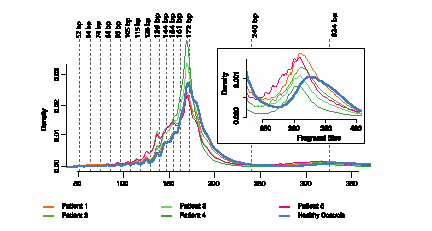
\includegraphics[width=0.9\linewidth]{Figures/intro/fragmentSizeDist}
\caption[Fragment size distribution of ctDNA]{Fragment size distribution of 5 high grade serous
ovarian carcinoma (HGSOC) patients and panel of healthy controls. The vertical dashed lines are placed on the fragment sizes between 52 and 172 bp where 10 bp periodicity is observed. The vertical lines at 240 and 324 bp show the range at which a shift in the di-nucleosomal peak occurs between HGSOC patients and healthy controls. The inset plot enlarges the density profile in the di-nucleosomal fragment length range. Figure adopted from \textcite{Markus2022}}\label{fig:ctdnaFragSize}
\end{figure}

Due to the different biological processes which can lead to the release of DNA from cancer cells, in addition to apoptosis, which is the main source of cfDNA from healthy cells, ctDNA has several biological differences to cfDNA. The most prominent features observed are distinct ctDNA fragmentation size patterns, fragment start sites, and fragment ends motives. While the preferred end motive and start site are heavily correlated, restricting the analysis to the lower tail of the mono- and di-nuclesomal peak of the fragment size distribution (74-155bp and 240-325bp) allowed a ctDNA tumour signal enrichment of at least 28\%. This is enrichment and the high periodicity of the distribution showed a high dependence on nucleosomal placement. All ctDNA features combined were shown to be able to predict the presence or absence of tumour DNA in a samples regardless of tumour type  (\autoref{fig:ctdnaFragSize}, \cite{Mouliere2018,Markus2022}). 


% background of sequencing DNA
\section[DNA sequencing]{DNA sequencing - when is next generation sequencing the current generation?}
\label{intro-sec:sequencing}

As we know the building blocks, that make DNA as well as the process and the enzymes responsible, we can synthesise DNA in vitro. By chemically modifying the nucleotides supplied to the synthesis process, the sequence of the copied strand can be analysed. The first method to make use of this used the lambda phage to fuse known ends for the primers needed for the reaction to the piece of DNA and supplied labelled nucleotides \cite{Padmanabhan1974}.This method was then superseded by "Sanger sequencing" after Frederick Sanger who with colleagues published this method in 1977, by adding \textbf{di}deoxynucleotides in a low concentration, the polymerase chain reaction would terminate trying to integrate these nucleotides and by labelling them radioactively or flourecently, a gel can be used to determine the sequence of a piece of DNA\cite{Sanger1975,Sanger1977}, which made the method better suited for larger scale projects.

However this method has multiple issues for modern research questions. Mostly, that it is fairly labour and time consuming to analyse multiple pieces of DNA at the same time and it is very challenging to sequence all the DNA of an organism. The human genome project, which was started in 1990 used machines which automated the Sanger sequencing procedure and it still took hundreds of researchers 13 years to complete the DNA sequence of just one human \cite{Lander2001,Venter2001}. Even though this was a very long project, it laid the ground work for the usage of the current sequencing technologies.

\subsection[Library preparation]{Library preparation - what we learned from using phages}
\label{intro-sec:libraryprep}

\begin{figure}[!ht]
\centering
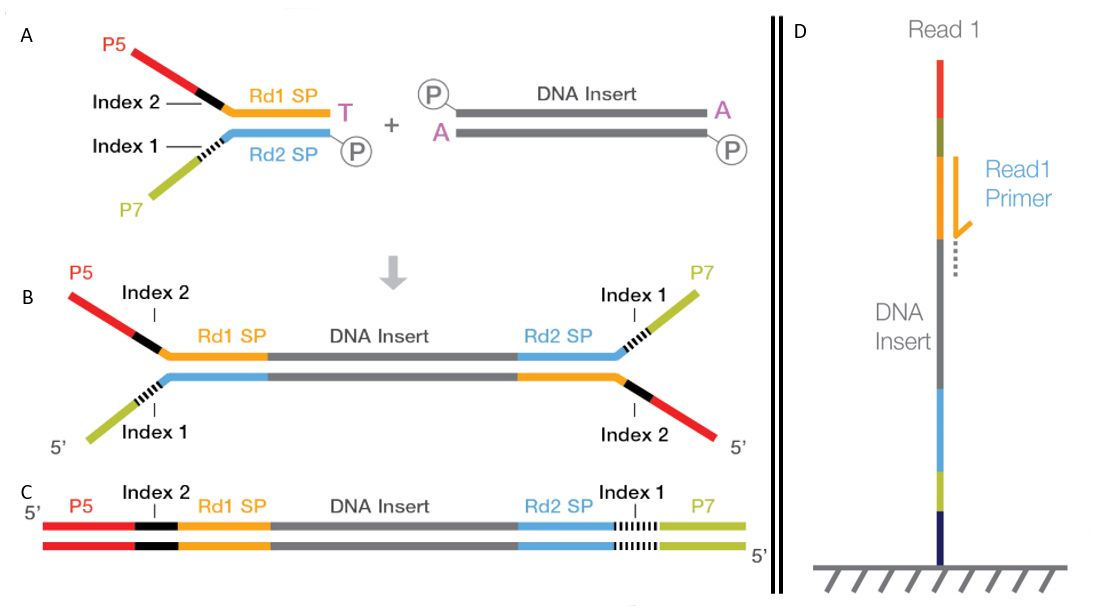
\includegraphics[width=.9\linewidth]{Figures/LibraryPreparation.png}
\caption[Library preparation for NGS]{Adapter ligation during library preparation. The adapters are added to the DNA insert during library preparation. A. The DNA insert is prepared by adding an A-tail and phosphorylation. B. The adapter complex which includes the P5/P7 flow cell binding adapter is added to the DNA insert. C. The DNA insert is ready for sequencing. D. The DNA insert binds to the flow cell for sequencing. Primers bind to the DNA insert to generate reads; \\Figure adapted from \href{https://sapac.support.illumina.com/bulletins/2020/12/how-short-inserts-affect-sequencing-performance.html}{"How short inserts affect sequencing performance"}\protect\cite{Illumina2020}}\label{fig:libraryprep}
\end{figure}

Library preparation is the name of the preprocessing step, which is done before it is sequenced with the current technologies. The first step to sequence DNA is to obtain the DNA, which is done by lysing the cells of interest, which disrupts the cell membrane and therefore spills all its contents. The then spilled DNA is fragmented into smaller pieces, by either restriction enzymes or sonication, to have a size of about between 200-800bp. These steps are not necessary when preparing sequencing of ctDNA, as discussed in \autoref{intro-sec:ctDNA}, the DNA is unbound and already digested into short fragments.
Once the DNA is ready, it is both phosphorelated as well as an A-tail is added, before the adapter complex is ligated. This enabled the DNA to bind to the flow cell which is covered with the reverse complement of the adapter \autoref{fig:libraryprep}. 

\subsection{Next generation sequencing}
\label{intro-sec:ngs}

\begin{figure}[!ht]
\centering
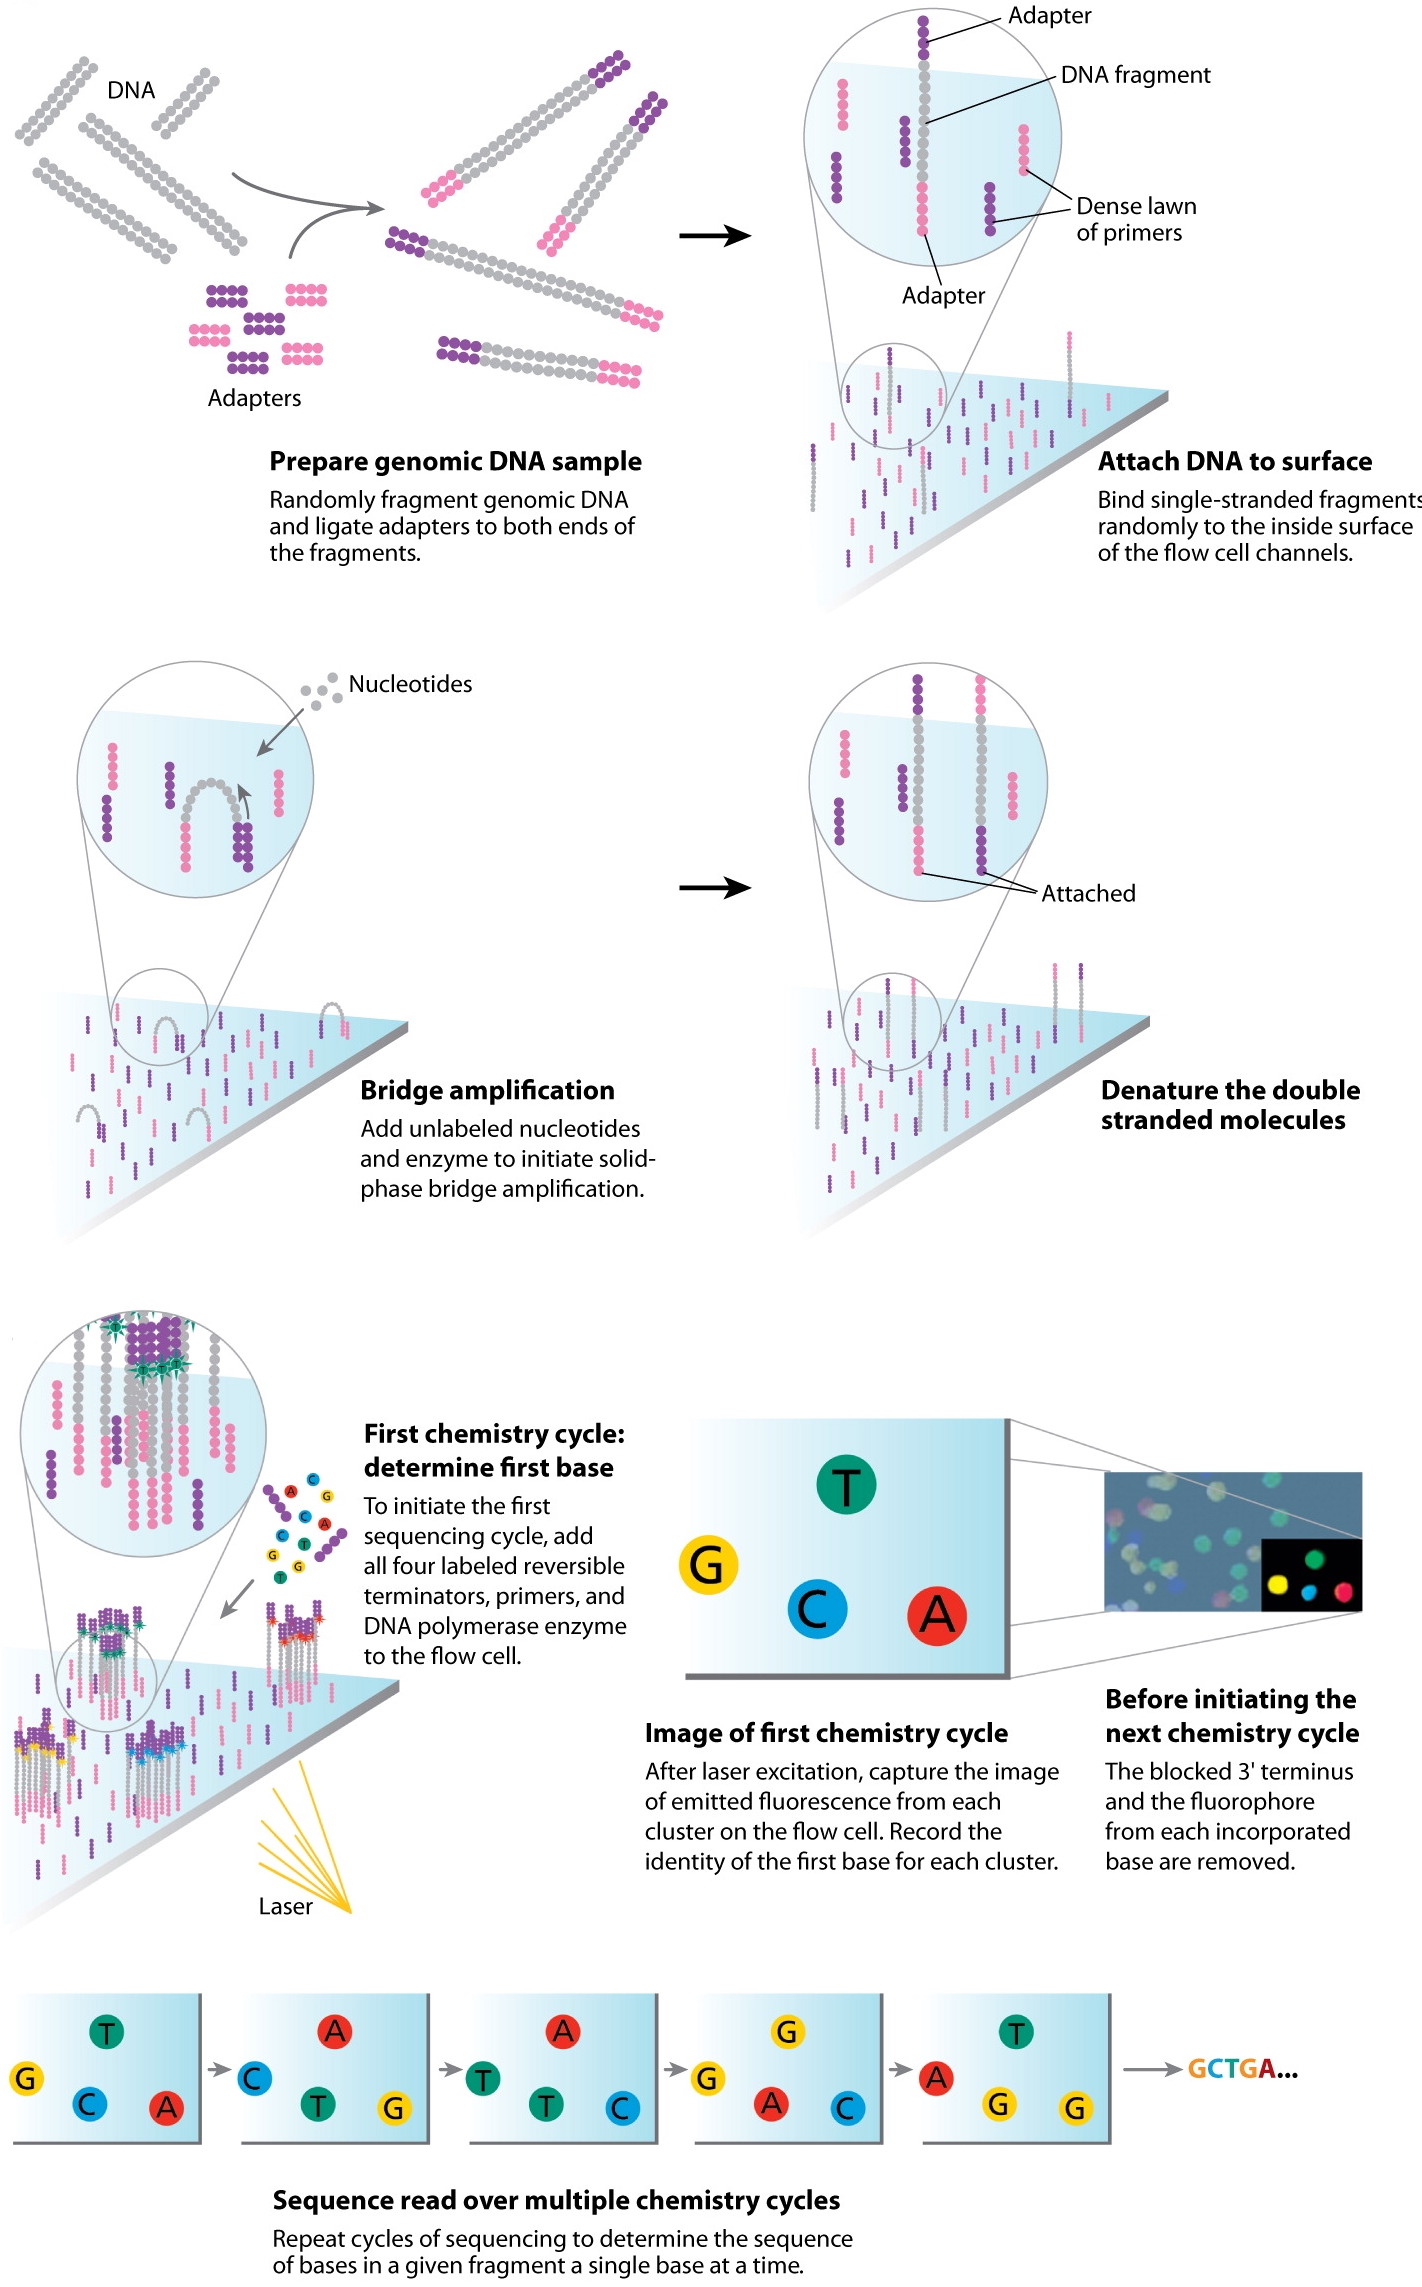
\includegraphics[width=.85\linewidth]{Figures/SequencingBySynthesis.jpg}
\caption[Sequencing by synthesis (Illumina)]{The Illumina sequencing-by-synthesis approach. Cluster strands created by bridge amplification are primed and all four fluorescently labeled, 3'-OH blocked nucleotides are added to the flow cell with DNA polymerase. The cluster strands are extended by one nucleotide. Following the incorporation step, the unused nucleotides and DNA polymerase molecules are washed away, a scan buffer is added to the flow cell, and the optics system scans each lane of the flow cell by imaging units called tiles. Once imaging is completed, chemicals that effect cleavage of the fluorescent labels and the 3'-OH blocking groups are added to the flow cell, which prepares the cluster strands for another round of fluorescent nucleotide incorporation; Figure adapted from \protect\citeauthor*{Mardis2008}\protect\cite{Mardis2008}}\label{fig:sequencingbysynthesis}
\end{figure}
%make sure the image comes as early as possible
\afterpage{\clearpage}

Next generation sequencing (NGS)is the coined term for basically any standard high-throughput sequencing performed, which includes exome, genome, transcriptome, protein-dna interactions (ChIP) and other epigenome studies. The term NGS is still widely used, even though it has been more than 10 years since the first NGS approach was commercially available. While in the beginning of next generation sequencing there were multiple approaches, the current lion share (80\% of sequencing data) of protocols use the Illumina short read sequencing by synthesis approach (\autoref{fig:sequencingbysynthesis})\cite{Mardis2008,Straiton2019}, which is based on the concept of alternating integration of florescently labelled nucleotides and imaging with a microscope (\autoref{fig:sequencingbysynthesis}) as well as multiplexing, where a DNA fragment is ligated to an index, which allows the sequencing of multiple samples at once \cite{Church1984,Church1988} as it is shown in \autoref{fig:libraryprep}. This method allows highly accurate determination of the sequence of a DNA fragment and depending on the flow cell and sequencing machine allows to sequence a whole genome in just 24h.

\subsection[Long read sequencing]{Long read sequencing - the "third" generation sequencing}
\label{intro-sec:lrs}
By now, multiple methods which broke free of the size limitations of NGS exist, which are commonly referred to as long read sequencing. Most of the current methods trade the very high accuracy of the second generation NGS methods for the capability of sequencing of sequencing huge continous strands of DNA (current record 2.3 Million bp \cite{Payne2018}) with normal library preparation ranging between 10-30 Kbp. 
These methods are expected to revolutionise our understanding of the highly repetitive elements that exist in the genome, such as the centromeres of chromosomes. Methods such as the direct molecule sequencing approach by Oxford Nanopore are even able to distinguish post transcriptional modifications on RNA\cite{Pratanwanich2021}.
So far, these methods however are still very expensive and as this work is dealing with ctDNA, which is highly fragmented, these methods offer only limited advantages over the short read sequencing, while being much more expensive.



% background of sequencing
\section[DNA analysis]{DNA analysis- what to do with the sequence}
\label{intro-sec:analysis}
The types of analysis that can be done with the output from the sequencing machine stretches far,  however, all methods need to first infer the location in the genome, the sequenced piece of DNA originated from. As the current methods randomly fragment the DNA (\autoref{intro-sec:libraryprep}), the genomic location information is completely lost. This process is referred to as mapping.

\subsection[Mapping]{Mapping - Ey man, where is my origin}
\label{intro-sec:mapping}
In this process, the fragments of DNA, which were sequenced, are assigned a genomic coordinate on the reference genome. This is only possible, due to the fact, that we have a resolved genome sequences (see~\autoref{intro-sec:sequencing}) for a high number of species. The location a sequenced piece of DNA fits to the reference genome might be unique, but it could also fit to multiple locations, due to highly repetitive regions or due to the existence of pseudo genes with almost 100\% identify. In addition to this, the reference genome might not accurately reflect the genome of the organism that has been sequenced. Each mapping position is therefore assigned a quality score, which reflects how likely it is the actual position of the sequence. As Illumina sequencers have the ability to sequence both ends of the DNA fragment, the position of the ends (read 1 and read 2) to each other can also be used to infer the quality, as they should be within a reasonable distance to each other (see \autoref{fig:libraryprep})

As this process is time consuming and the exact location of the fragment might not be as important, there exists a subset of tools called pseudo-mapper, which are based on $k$-mers, which are predefined DNA sequences of length $k$, which help to identify certain regions of interest. These tools are especially common for RNAseq, where the exact location of a read doesnt matter, only that the read is within a gene \cite{Bray2016,Patro2017}.

\subsection[Variant calling]{Variant calling - spot the distance}
\label{intro-sec:variantcalling}


% background of lung cancer
\section{Cancer}
\label{intro-sec:cancer}

While cancer is a massively heterogenous disease, as it can arise through a multitude of ways in almost any tissue, there are a some fundamental defining features, which most, if not all malignancies acquire, before they are truly cancers . The original characteristics comprise 
\begin{enumerate*}
	\item Sustaining proliferative signaling
	\item Evading growth suppressors
	\item Activating invastion and metastasis
	\item Enabling replicative immortality
	\item Inducing angiogenesis
	\item Resisting cell death
\end{enumerate*} (\autoref{fig:oldhallmarks}). 
These hallmarks were long considered the core of tumour development and the authors themselves hypothesised, that these core mechanics allow us to condense the complexity that cancer displays, both in the clinic as well as in labs, with a small set of rules, which all cancers have to obey \cite{Hanahan2000}. In their exact words: ``We foresee cancer research developing into a logical science, where the complexities of the disease, described in the laboratory and clinic, will become understandable in terms of a small number of underlying principles``

\begin{figure}[!ht]
\centering
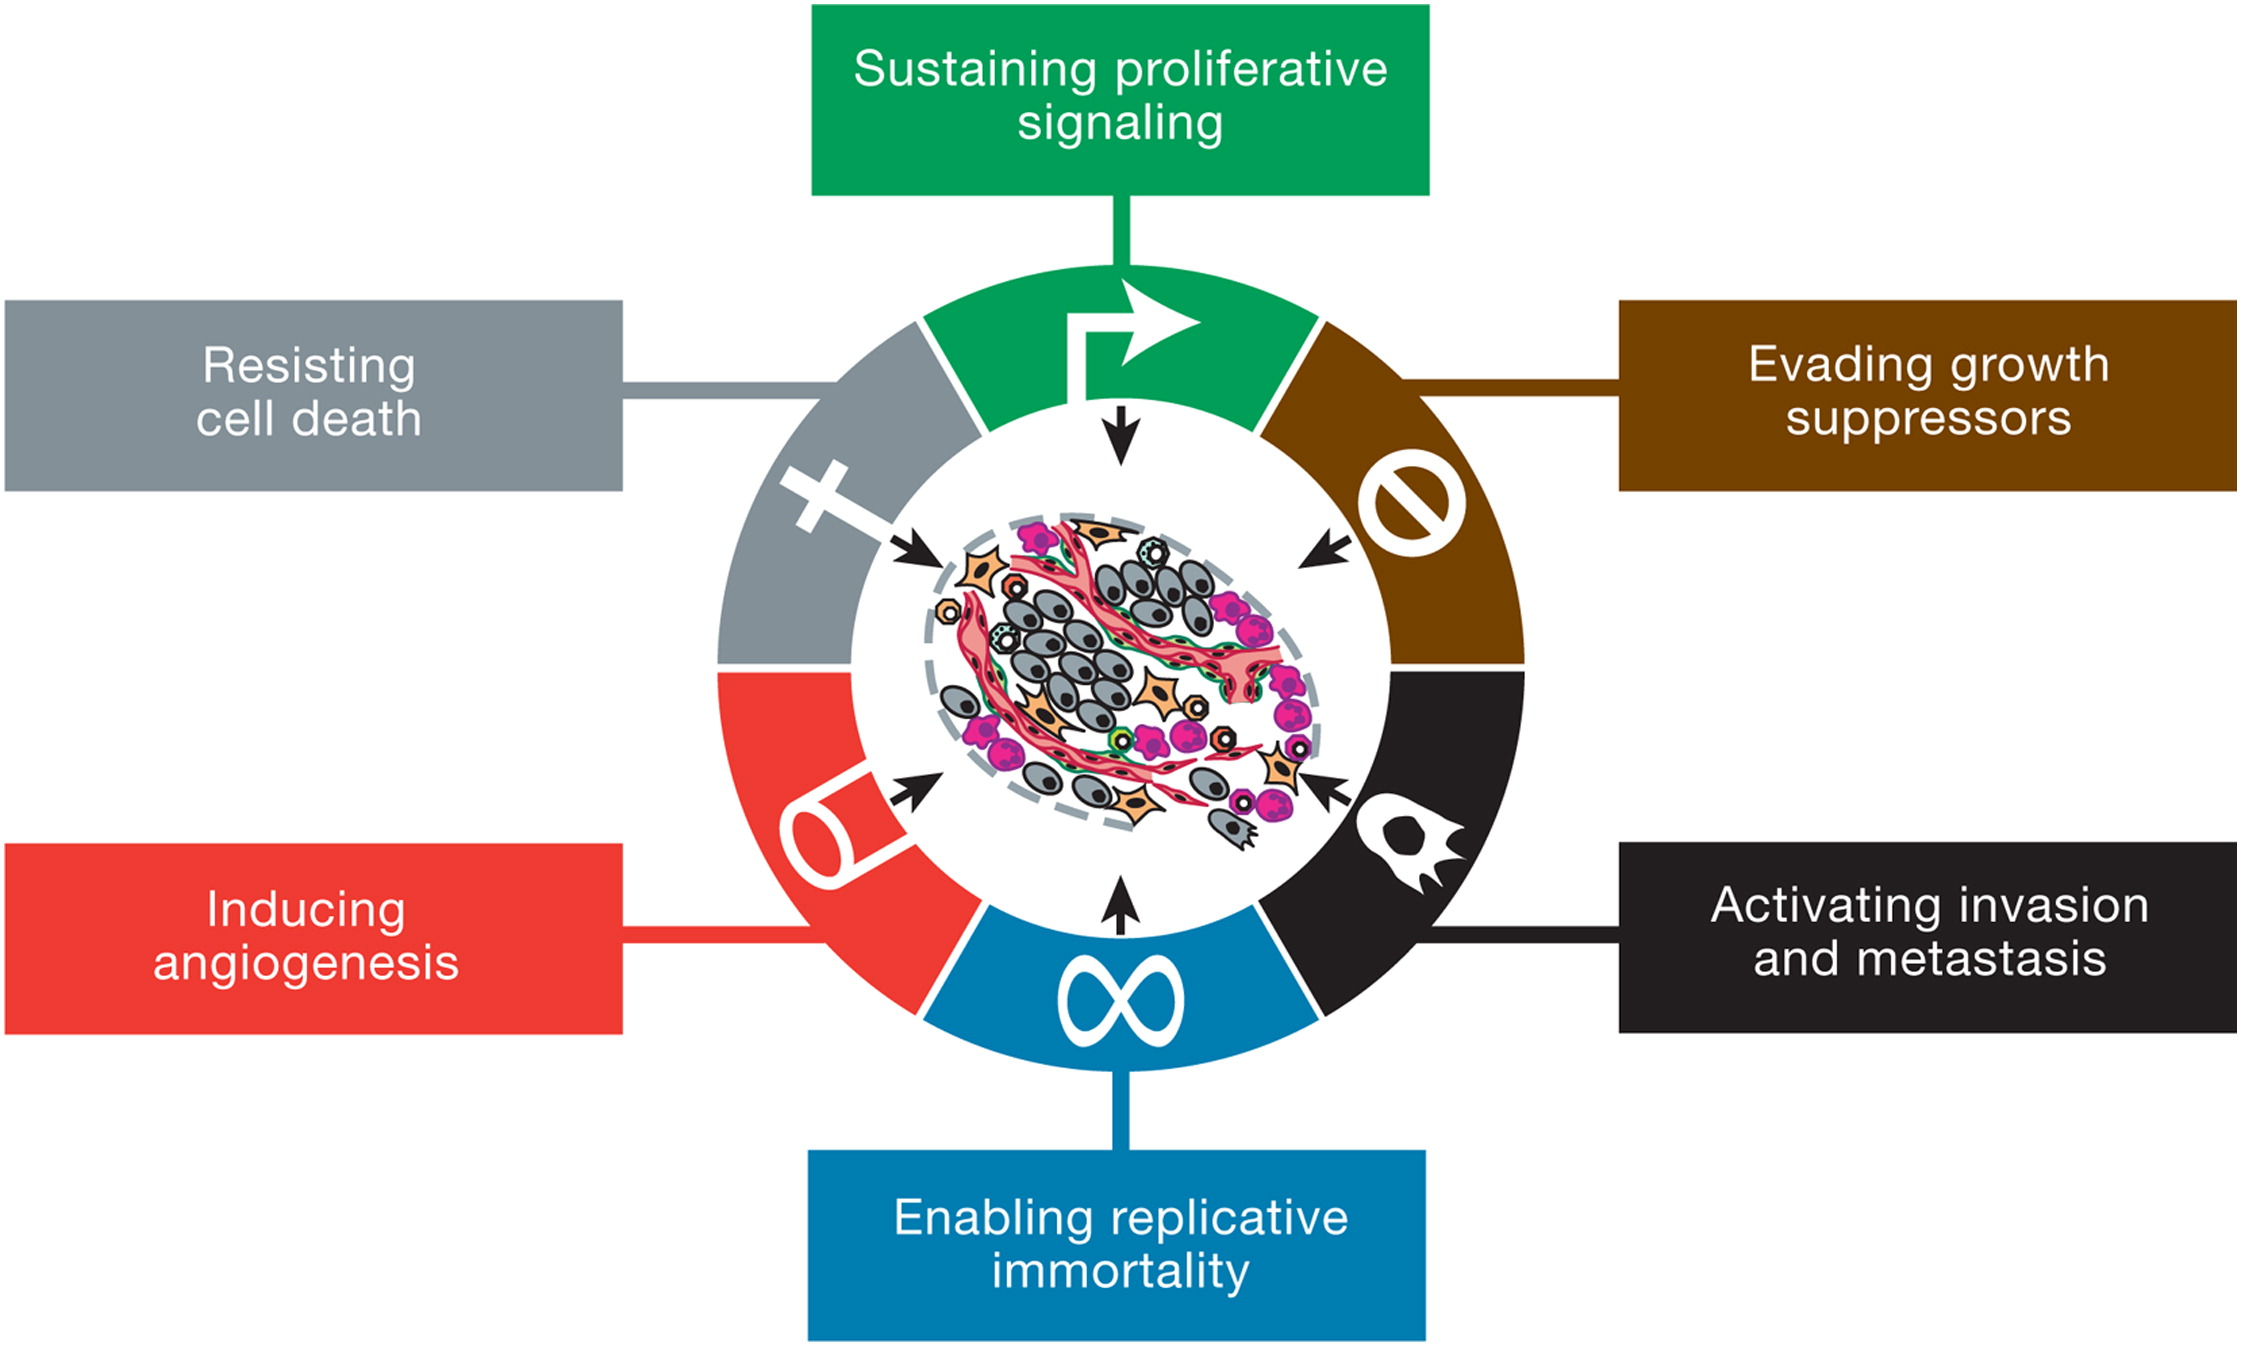
\includegraphics[width=.95\linewidth]{Figures/oldHallmarksCancer.jpg}
\caption[Original hallmarks of cancer]{Acquired capabilities of cancer; Functional capabilities acquired by most cancers during their development; Figure adapted from \protect\citeauthor*{Hanahan2000}\protect\cite{Hanahan2000}}\label{fig:oldhallmarks}
\end{figure}

However, with 11 years of additional research into the topic, more hallmarks have been found and the original list was revised by the authors to contain additional characteristics, namely 
\begin{enumerate*}
\item Avoiding immune destruction
\item Tumour-promoting inflamation
\item Genome instability and mutation
\item Deregulating cellular energetics
\end{enumerate*}
(\autoref{fig:newhallmarks}) \cite{Hanahan2011}. And even then a few years later, even more hallmarks e.g. metabolic rewiring are now considered a part of the characteristics of cancer \cite{Fouad2017}.

\begin{figure}[!ht]
\centering
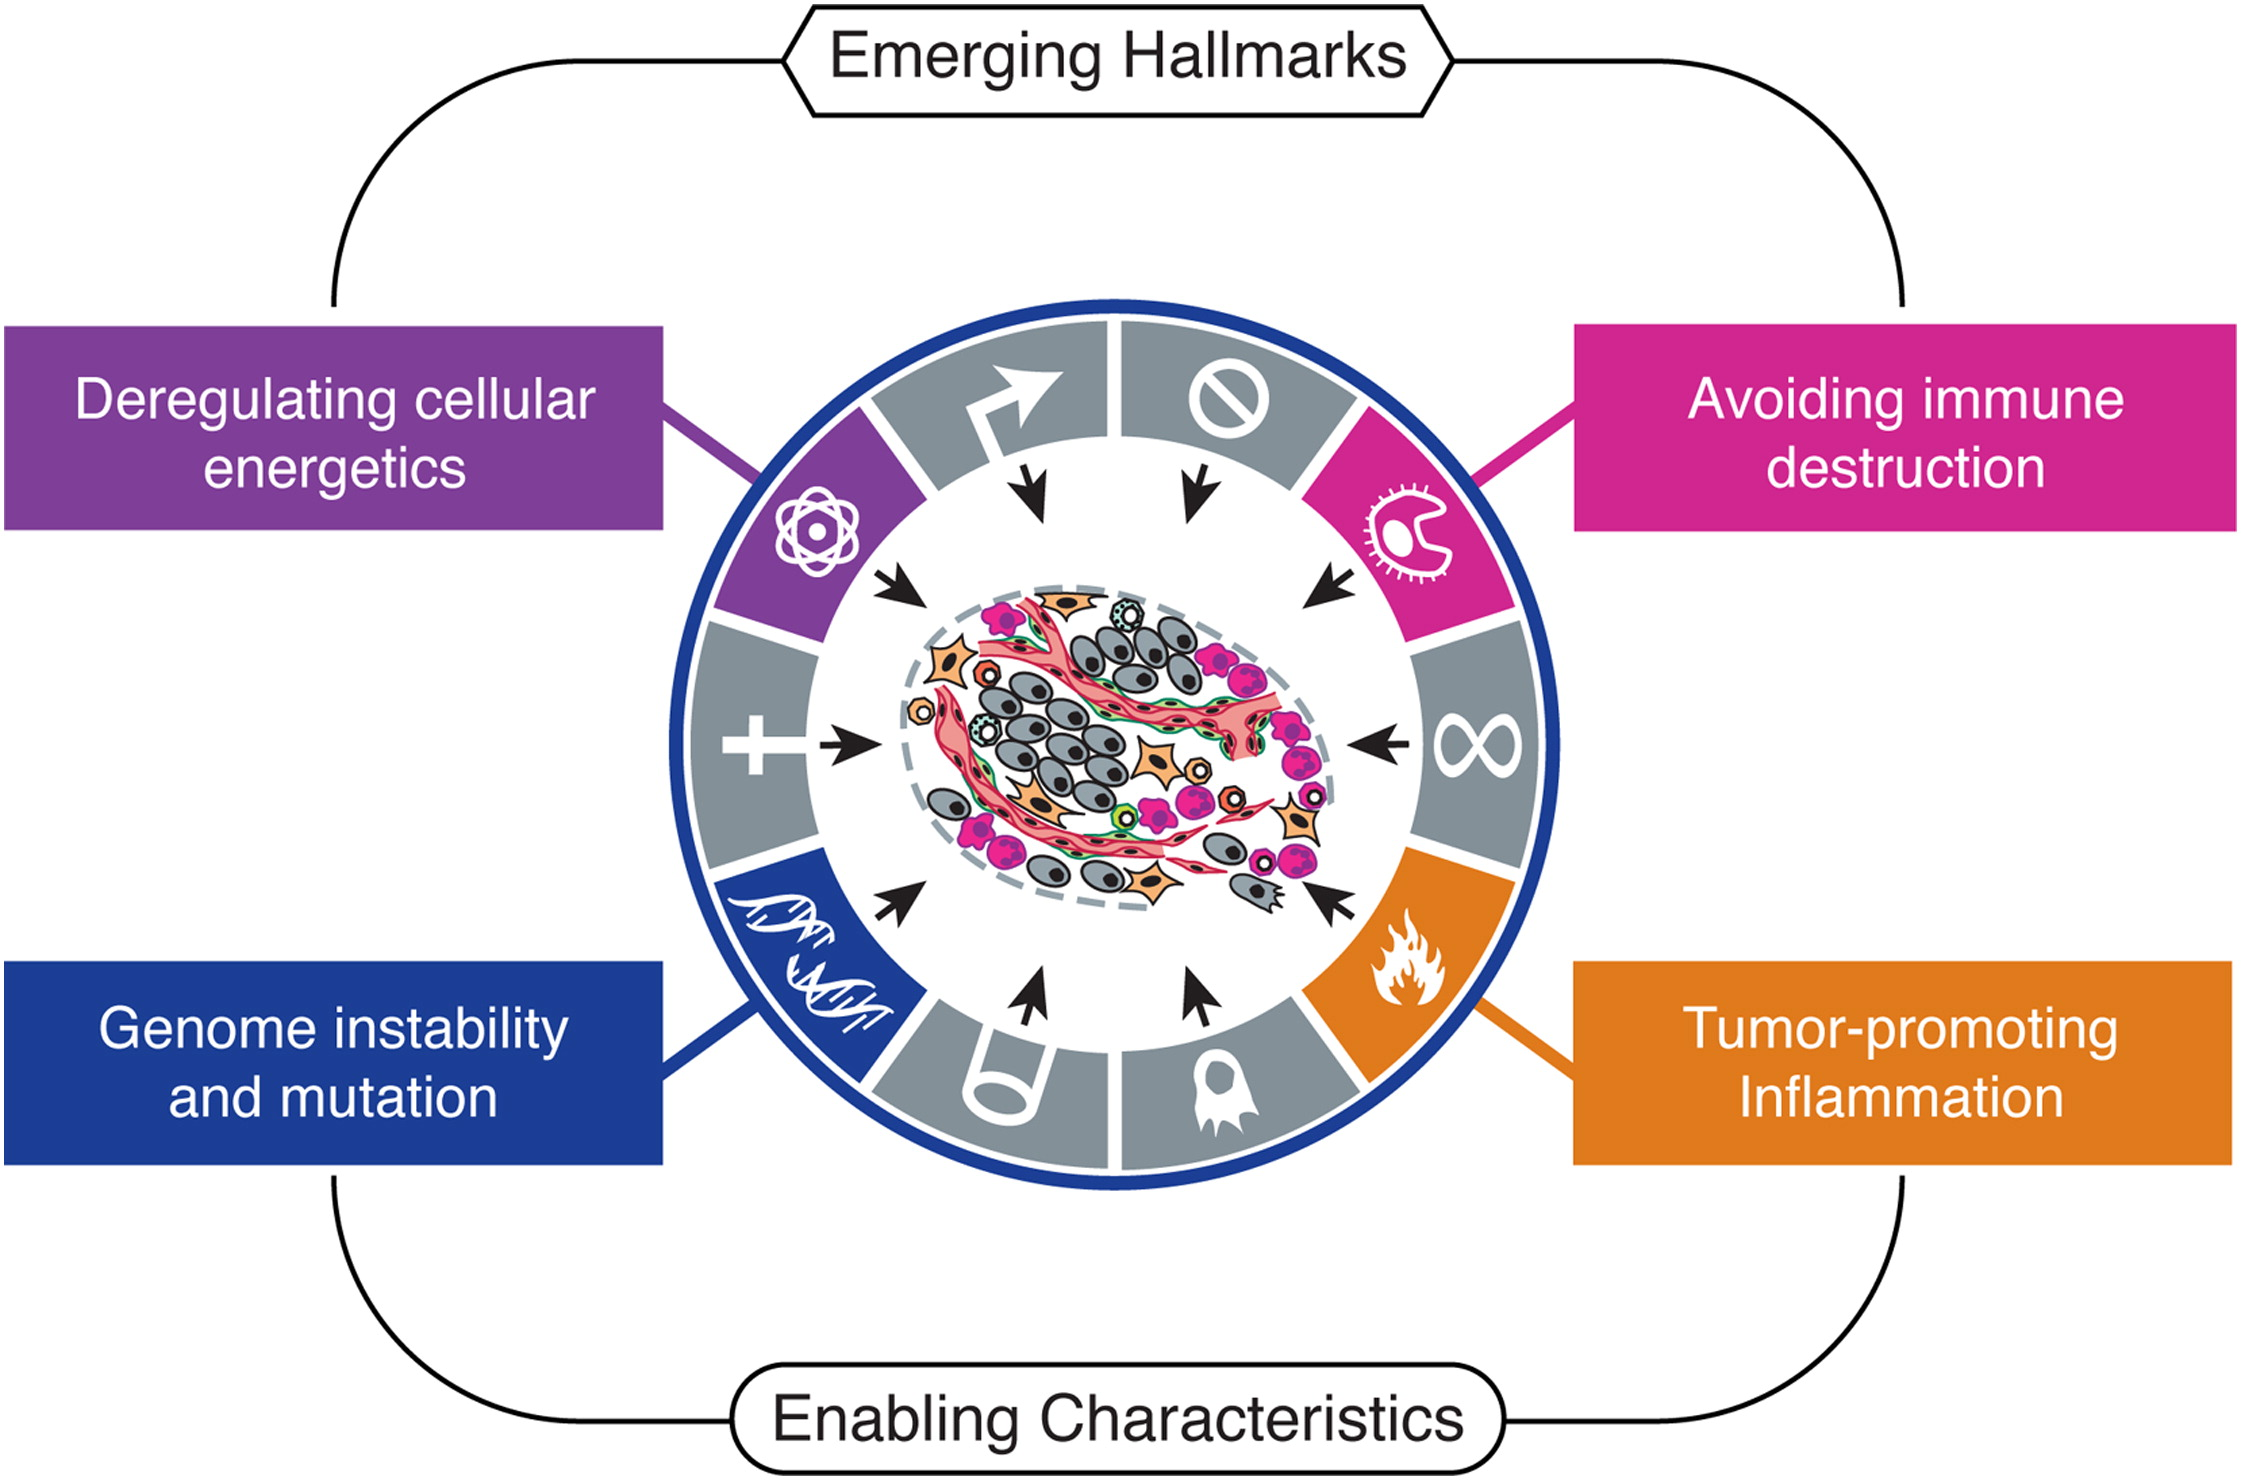
\includegraphics[width=.95\linewidth]{Figures/newHallmarksCancer.jpg}
\caption[New hallmarks of cancer]{Emerging hallmarks and enabling characteristics of cancer; updated version of the hallmarks figure (\autoref{fig:oldhallmarks}) with ; Figure adapted from \protect\citeauthor*{Hanahan2011}\protect\cite{Hanahan2011}}\label{fig:newhallmarks}
\end{figure}

So while the original set of the hallmarks was not sufficient or complete, it offered a good attempt at abstraction of biological concepts to describe cancers. In the following pages, I will outline each of those hallmarks and how it influences my research.

\todo[inline, color=red]{describe the hallmarks}

\subsubsection{Sustaining proliferative signaling - there are no breaks on the train}

\subsubsection{Evading growth suppressors}

\subsubsection{Activating invasion and metastasis - look at me... I am the organism now}

\subsubsection{Enabling replicative immortality}

\subsubsection{Inducing angiogenesis}

\subsubsection{Resisting cell death}

\subsection{Lungcancer}
\label{intro-sec:lungcancer}

With around 1.6 million deaths world-wide each year, lung cancer is the number one cause of cancer death \cite{Siegel2018}. Every year about twelve thousand Australians get diagnosed with lung cancer. These cases can be generally split into two groups: small cell lung cancers (SCLC) and non-small cell lung cancers (NSCLC), which account for around 15\% and 85\% of cases, respectively. The majority of NSCLC are either lung adenocarcinoma or lung squamous cell carcinoma \cite{Molina2008}. Even though smoking is highly associated with lung cancers, there is a big group of never smokers, with a high risk of lung cancers in East Asia, especially women, which is correlated with outside influences like pollution and occupational carcinogens and paired with genetic susceptibility \cite{Sun2007}.
This group usually shows \textit{EGFR} (epidermal growth factor receptor) driven tumours. EGFR is a transmembrane receptor tyrosine kinase, which is usually only expressed in epithelial, mesenchymal, and neurogenic tissue, but its overexpression in other tissues is a hallmark of many human malignancies, not just NSCLC.

\todo[inline]{Possibly change this to cancer in general}

%% original abstract
%Approximately 50% of patients with non-small cell lung cancer (NSCLC) develop acquired resistance to EGFR tyrosine kinase inhibitors (TKIs) through mutations in EGFR T790M. Maintaining a dynamic balance between T790M positive and negative clones offers an opportunity to delay the emergence of resistance and improve disease outcomes. It is now possible to quantify EGFR mutations using circulating tumour DNA (ctDNA) which can provide a surrogate measure of clonal populations within tumours. This project will utilise next generation sequencing (NGS) of tumour tissue and ctDNA in patients treated with EGFR TKIs to study clonal evolution patterns and predict optimal treatment approaches to delay therapeutic resistance.

% thesis overview
\section{Thesis overview and aims}
\label{intro-sec:overview}

While tumour heterogeneity is a well accepted concept by now, there is a need for computational methods assessing and visualising this heterogeneity. This work aims to contribute to this unmet need by developing three different custom made tools to infer and monitor tumour heterogeneity. I have completed the work in the following three parts:

\begin{enumerate}
	\item Development of two joint somatic variant calling workflows and the impact of these on downstream analysis (\autoref{ch:variantcalling}). 
	\item Analysis of five rapid autopsy probands with state of the art methods to investigate tumour heterogeneity and development of a mitochondrial based phylogeny reconstruction method (\autoref{ch:cascade}). 
	\item Development of a read-centric method to detect somatic mutational signatures from low coverage whole genome sequencing (\autoref{ch:mmf}).
\end{enumerate}
 

% includes all the variant calling subheadings as well as a short summary of the thing

\begin{savequote}[85mm]
``It is the main source of our mistakes,  when making making decision, that we only look at life piece by piece and not as a whole.``
\qauthor{--- Lucius Annaeus Seneca, \textit{Epistulae morales ad Lucilium}}
\end{savequote}

\chapter[Joint somatic variant calling]{Joint somatic variant calling - if germline can do it, so can we}
\label{ch:variantcalling}

%\epigraph{``It is the main source of our mistakes,  when making making decision, that we only look at life piece by piece and not as a whole.``}{--- \textup{Lucius Annaeus Seneca}, Epistulae morales ad Lucilium}


% setting up the concept of variant calling
\section{Introduction}
\label{variantcalling-sec:intro}
In 2018, at the start of the work presented in this thesis, we observed a difference in methodology  between germline and somatic variant calling methods. Where all "modern" germline variant callers, like Strelka2 \cite{Kim2018}, HaplotypeCaller \cite{Poplin2017}, DRAGEN \cite{Miller2015} and DeepVariant \cite{Poplin2018},  have the built-in capability to jointly call multiple related samples, for example from family trios, virtually no somatic variant caller had this functionality. 

The joint analysis of smaller cohorts improves the performance of germline variant calling methods significantly, by allowing to assess technical artefacts, which might be unique for the individual sequencing machine or the researcher handling the DNA \cite{Schirmer2016,Stoler2021}. Additionally, as certain parts of the genome are more problematic to sequence (\autoref{intro-sec:sequencing}) and map (\autoref{intro-sec:mapping}), a ``control`` sample can help to distinguish if a certain observed change occurring frequently is a technical issue or in fact a real change.

For somatic variant calling, this concept has been adopted on in the genome analysis toolkit (GATK) \cite{BrianOConnor2020} to allow the use of panel of normals (PON), which contains frequently seen changes in healthy (``normal``) individuals analysed with the same sequencing technology \cite{GATKTeam2021}. Although, in contrast to the  more intricate model for the germline equivalent, this is a post processing step of the analysis. Mutect2, which is the most recent somatic variant calling algorithm provided by the Broad institute, also provides a multi-sample mode, for which all tumour samples need to be from the same patient, either related longitudinally or spatially \cite{GATKTeam2020}. However, this mode is not very well publicised and all tutorials released by the developers state that ``there is currently no way to perform joint calling for somatic variant discovery`` \cite{GATKTeam2021a}. So while all methods in the GATK are considered a beta feature, the multi sample mode needs to be used with care.

There are only two methods currently, which have documented and published capabilities to jointly analyse tumour samples from the same patient to call somatic variants. The first one is a specialised method built on a joint bayesian model for SNVs that occur in multiple samples called multiSNV \cite{Josephidou2015}. However, it has multiple shortcomings, which make it not usable for our data. First, as the name suggests, the method can only jointly evaluate SNVs and completely ignores INDELs and structural variants, which would be acceptable for the superior performance it provides. However, multiSNV was optimised only for WES and not for the very deep WGS that is now available and part of this thesis. This mismatch of input types means exceptionally high runtimes on our data. Even with custom parallelisation that was attempted in this work, the predicted runtime for just one multi sample patient would have been longer than 3 years. This shows, that while multiSNV was a great step forward at the time, there is a real need for new methods to stem the tide of sequencing data available due to the ever decreasing sequencing cost.

multiSNV has been the only software available for multi sample analysis for almost five years, but during this work, superFreq \cite{Flensburg2020} was published. It combines all standard analysis steps for tumour analysis, like quality assessment, variant calling, copy number analysis and clonal deconvolution, into one program and is even able to jointly analyse samples. However, similar to multiSNV, its focus during optimisation and development was on WES and RNAseq data, so when applied to our data, we could not find a server node with enough memory to execute the workflow.

This then prompted us to investigate possible workflows to enable the analysis of high depth WGS, which we estimate to become more and more normal, with the ever dropping prices of sequencing. The following sections will show the development and validation of the joint variant calling methods as described in \textcite{Hollizeck2021} (\autoref{variantcalling-sec:publication}), additional analysis on the impact of the joint variant calling on downstream analysis (\autoref{variantcalling-sec:downstream}), longitudinal analysis (\autoref{variantcalling-sec:longitudinal}) and clonal deconvolution (\autoref{variantcalling-sec:clonal}) and lastly information on the usage of the methods by others in the research community (\autoref{variantcalling-sec:usage}).



% the link to the publication
\section{Publication}
\label{variantcalling-sec:publication}

The full publication about joint somatic variant calling can be found at \href{https://doi.org/10.1093/bioinformatics/btab606}{\nolinkurl{https://doi.org/10.1093/bioinformatics/btab606}} and non-journal formatted version is also attached as \autoref{ch:appendixManuscript} with all supplementary methods.

References to supplementary data will be prefixed with the letter \ref{ch:appendixManuscript} for figures and methods taken from the publication and \ref{A:ch:jsvSupp} for additional data generated for this work.

\subsection{Summary}
To enable highly sensitive, fast and accurate variant detection from multiple related tumour samples, we have developed joint variant calling extensions to two widely used single-sample algorithms, FreeBayes \parencite{Garrison2012} and Strelka2 \parencite{Kim2018}. Using both simulated and clinical sequencing data, we show that these workflows are highly accurate and can detect variants at much lower variant allele frequencies than other commonly used methods.

\subsection{FreeBayesSomatic workflow}
The original FreeBayes algorithm can jointly evaluate multiple samples, but routinely it does not perform somatic variant calling on tumour-normal pairs. We introduce FreeBayesSomatic which allows concurrent analysis of multiple tumour samples by adapting concepts from SpeedSeq \parencite{Chiang2015} which differentiates the likelihood of a variant between tumour and normal samples instead of imposing an absolute filter for all variants called in the normal. Hence, for each genotype (GT) at SNV sites, FreeBayesSomatic first calculates the difference in likelihoods (LOD) between the normal (\autoref{eq:01}) and the tumour (\autoref{eq:02}) samples genotype likelihoods (GL) with g$_{0}$ describing the reference genotype.


\begin{align}
\text{LOD}_{\text{normal}} &= \max_{g_i \in \text{GT}} \left( \text{GL}(g_0) - \text{GL}(g_i) \right) \label{eq:01}\\
\text{LOD}_{\text{tumour}} &= \min_{s \in \text{Samples}} \left( \min_{g_i \in \text{GT}} \left( \text{GL}_s(g_i) - \text{GL}_s(g_0) \right) \right) \label{eq:02}\\
\text{somaticLOD} & := \left( \text{LOD}_{\text{normal}} \geq 3.5 \land \text{LOD}_{\text{tumour}} \geq 3.5 \right) \label{eq:03}
\end{align}
%we have to specify them individualluy here, because align doesnt really allow it
\myequation[\ref{eq:01}]{FreeBayesSomatic: LOD$_{normal}$}
\myequation[\ref{eq:02}]{FreeBayesSomatic: LOD$_{tumour}$}
\myequation[\ref{eq:03}]{FreeBayesSomatic: somaticLOD definition}

Next, the variant allele frequencies (VAF) in both the tumour and the normal samples are compared at each site.


\begin{align}
\text{VAF}_{\text{tumour}} &= \max_{s \in \text{Samples}} ( \text{VAF}_s) \label{eq:04}\\
\text{somaticVAF} & := \left( \text{VAF}_{\text{normal}} \leq 0.001 ~\lor \right. \nonumber \\
 & \left. ( \text{VAF}_{\text{tumour}} \geq 2.7 \cdot \text{VAF}_{\text{normal}}) \right) \label{eq:05}
\end{align}
\myequation[\ref{eq:04}]{FreeBayesSomatic: VAF$_{tumour}$}
\myequation[\ref{eq:05}]{FreeBayesSomatic: somaticVAF definition}

A variant is classified as somatic when both somatic LOD as well as somatic VAF pass the criteria somaticLOD (\autoref{eq:03}) and somaticVAF (\autoref{eq:05}).

The thresholds chosen for both LOD and VAF calculations were previously fitted by the blue-collar bioinformatics workflow for the ``DREAM synthetic 3`` dataset using the SpeedSeq likelihood difference approach \parencite{Chapman2020} and were selected to identify high confidence variants.

\subsection{Strelka2Pass workflow}
In contrast to FreeBayes, whilst Strelka2 has a multiple-sample mode for germline analysis and tumour-normal pair somatic variant calling capabilities, it cannot jointly analyse multiple related tumour samples. We enable this feature by adapting a two-pass strategy previously used for RNA-seq data \parencite{Veeneman2015}. First, somatic variants are called from each tumour-normal pair. All detected variants across the cohort are then used as input for the second pass of the analysis, where we re-iterate through each tumour-normal pair but assess allelic information for all input genomic sites.

The method re-evaluates the likelihood of each variant, by integrating every genotype from each tumour-normal pair. This step can "call" a variant ($v$) in a sample that initially did not present enough evidence to pass the Strelka2 internal filtering using two conditions: 1) if this variant was called as a proper "PASS" by Strelka2 in any other tumour sample, or 2) if the integrated evidence for this variant across all tumour-normal pairs reached a sufficiently high level. The second condition was based on the somatic evidence score (SomEVS) reported by Strelka2, which is the logarithm of the probability of the variant $v$ being an artefact.

\begin{equation}
p_{error}(v) = 10^{\left( \frac{-\text{SomEVS}(v)}{10} \right)} \label{eq:06}
\end{equation}
\myequation[\ref{eq:06}]{Strelka2Pass: pairwise error probability}

While the germline sample is shared between all processes, we can approximate these individual probabilities as being independent, since one variant calling process is agnostic of the other. Hence, we derive the following:

\begin{equation}
p_{error}(v_{s_1},v_{s_2},\ldots,v_{s_n}) = \prod_{s \in \text{Samples}} p_{error}(v_{s}) \label{eq:07}
\end{equation}
\myequation[\ref{eq:07}]{Strelka2Pass: joint error probability}

And therefore:

\begin{equation}
\text{SomEVS}(v_{s_1},v_{s_2},\ldots,v_{s_n}) = \sum_{s \in \text{Samples}} \text{SomEVS}(v_{s}) \label{eq:08}
\end{equation}
\myequation[\ref{eq:08}]{Strelka2Pass: joint SomEVS}

This allows the summation (\autoref{eq:08}) of the SomEVS score across all supporting variants to assign a "PASS" filter, if it reached a joint SomEVS score threshold. This threshold can be set by the user and is 20 by default, which corresponds to an estimated error rate of 1\%. These "recovered" variants need to pass a set of additional quality metrics related to depth of coverage, mapping quality and read position rank sum score.

As an additional improvement, we also built multiallelic support into Strelka2 which originally only reports the most prevalent variant at a specific site. Within the two-pass analysis, we reconstruct the available evidence for a multiallelic variant at a called site from the allele-specific read counts and report the minor allele at this site, if there is sufficient support from other samples. This method allows recovery of minor alleles only if another sample has this variant called by Strelka2, as SomEVS scores are not available for minor alleles.


\subsection{Validation}

While the development of new methods can challenge previous assumptions and allow to challenge previous ruled, all methods need be validated against the current gold standard methods in the field with data which allows objective measurements. For germline variant calling, there have been multiple community lead challenges and specifically designed test datasets, but there is currently no somatic variant calling equivalent. This issue is even more pronounced for our method, as we do not only need a tumour-normal pair, but we need the multiple tumour samples in the dataset to be related. To allow a fair comparison, we first generated a fully synthetic dataset, where every variant is known and fully defined (\autoref{variantcalling-sec:simdata}) to allow a general performance assessment of the methods. Then to ensure that these metrics also hold true in real world data, we then re-analysed previously published datasets which have orthogonal validation in the form of targeted amplicon sequencing (TAS) (\autoref{variantcalling-sec:realdata}).

\begin{figure*}[!tpb]
\centering
  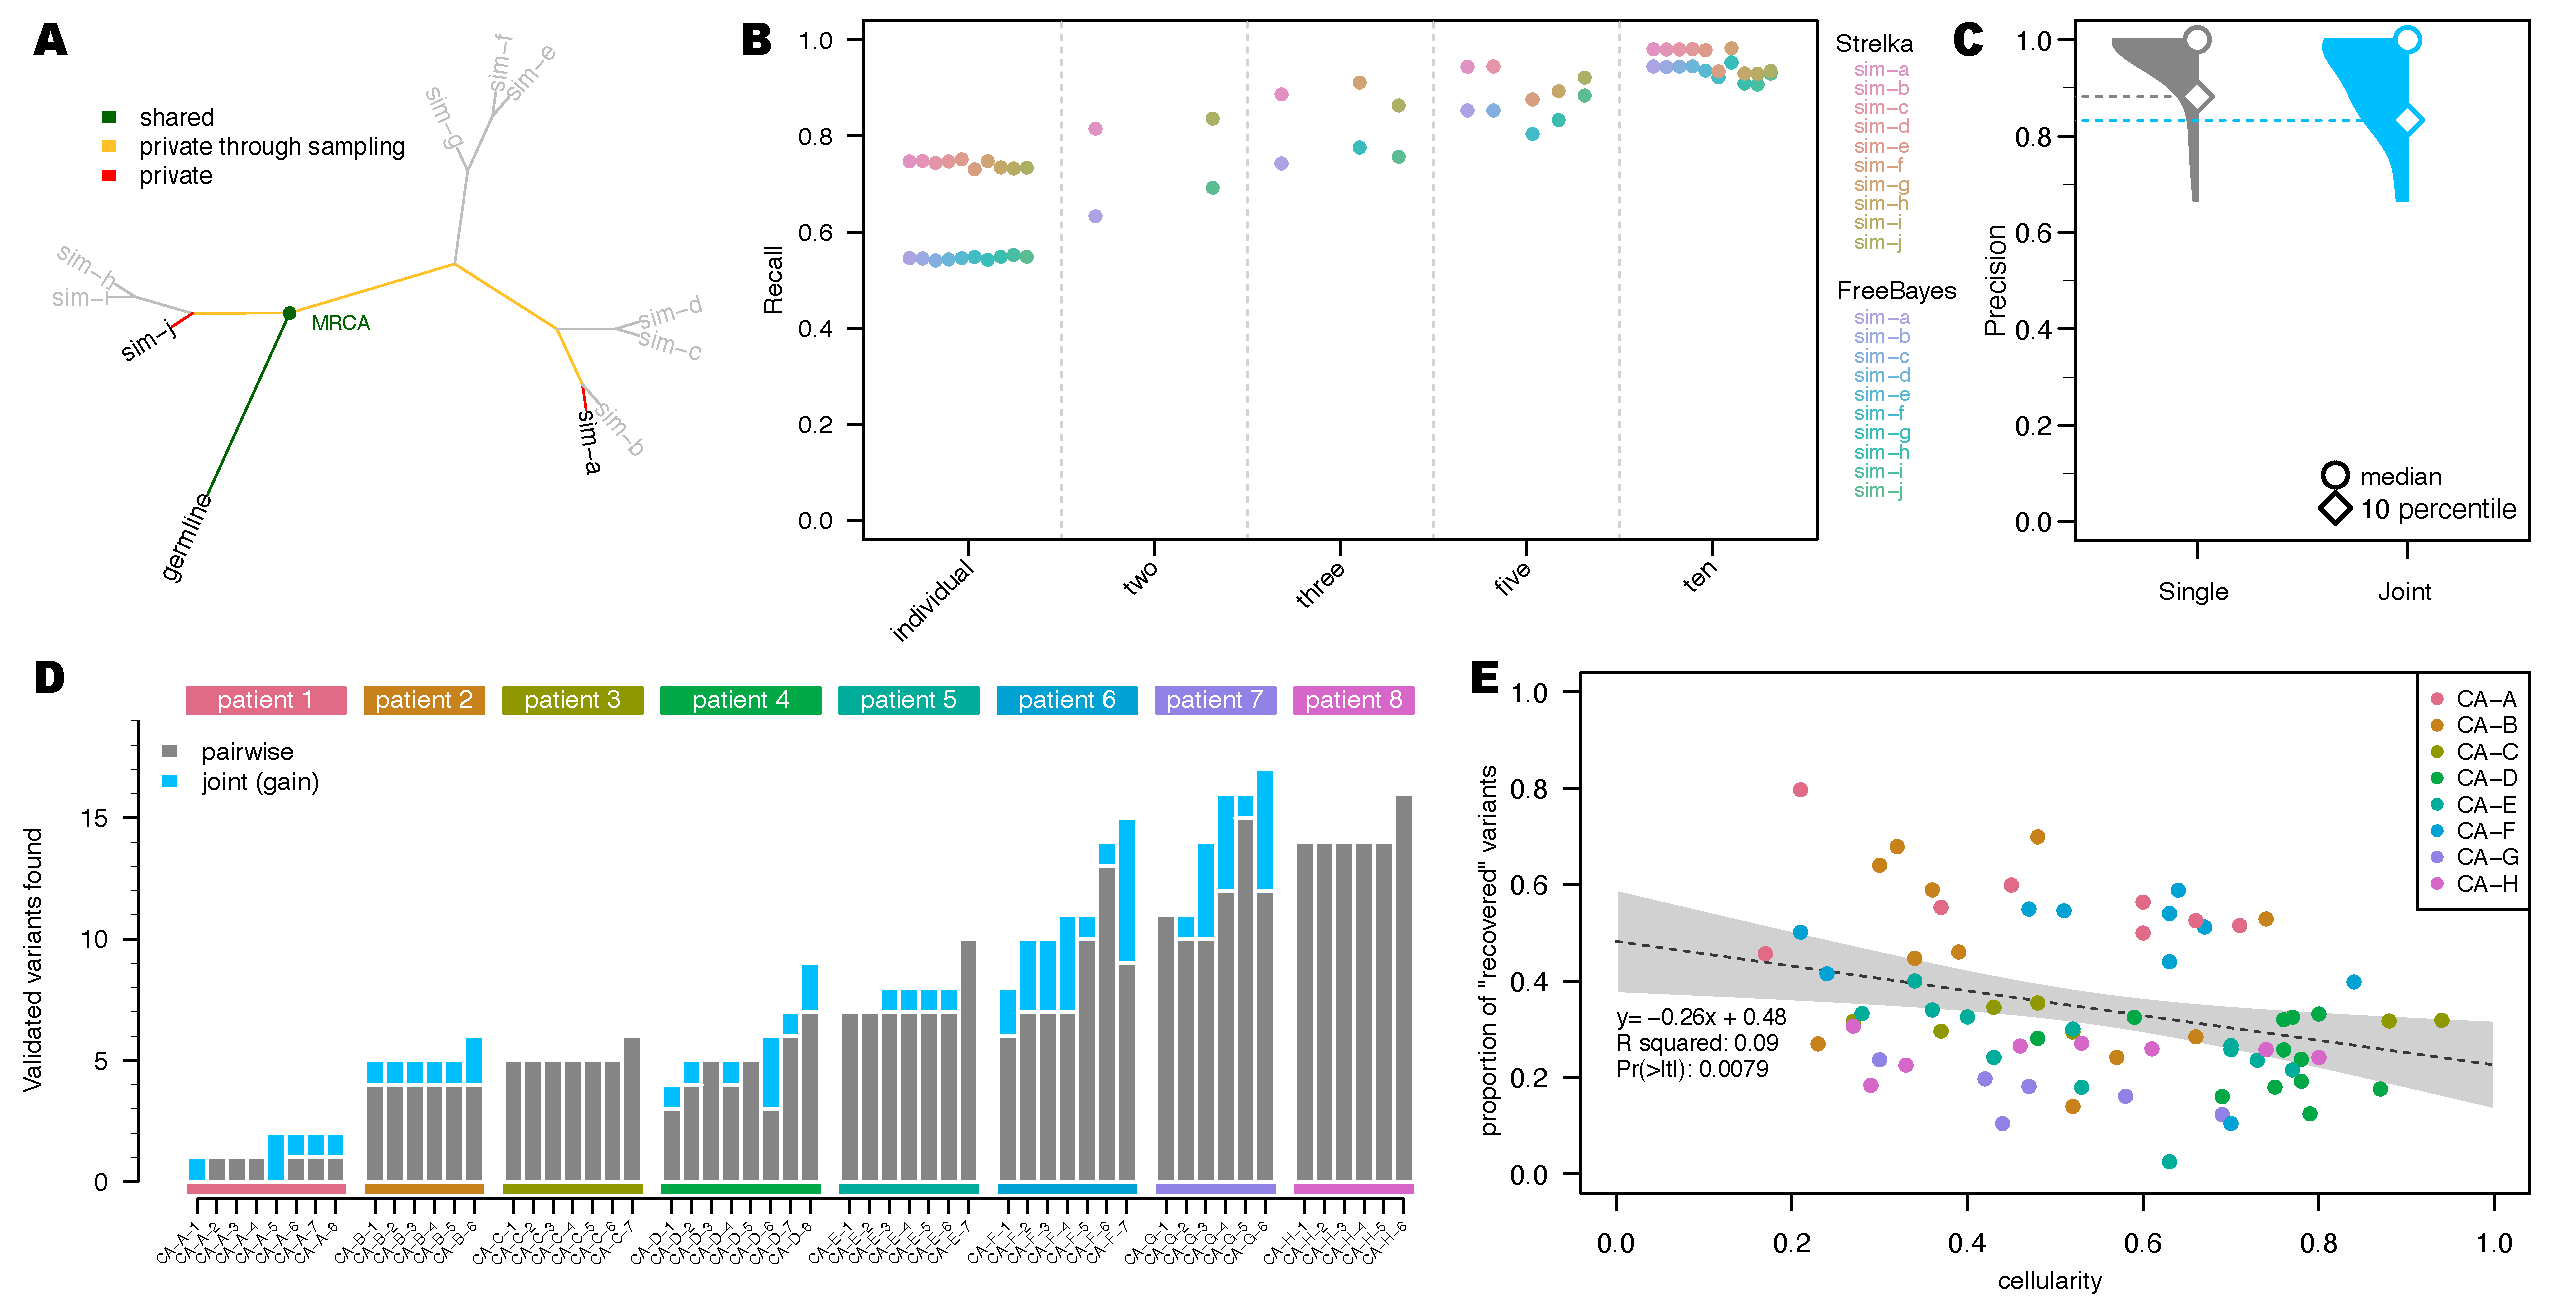
\includegraphics[width=\textwidth]{Appendices/Variantcalling/Figure_1}\vspace*{-12pt}
  \caption[Comparison of joint multi-sample and single tumour-normal paired variant calling methods]{Comparison of joint multi-sample variant calling and single tumour-normal paired calling methods; A) Simulated phylogeny highlighting two samples with high evolutionary distance (sim-a and sim-j) where MRCA denotes the most recent common ancestor. B) Recall estimates of FreeBayes and Strelka2, run in individual tumour-normal paired and joint calling configurations using two (sim-a and sim-j), three (sim-a, sim-g and sim-j), five (sim-a, sim-c, sim-f, sim-h and sim-j) and all ten tumour samples. C) Precision of Strelka2 and D) Number of variants called by Strelka2 run in both tumour-normal paired (grey) and added with joint calling configurations (blue), which have been validated by targeted amplicon sequencing (TAS). E) Correlation between cellularity and proportion of variants found only with joint calling using Strelka2Pass for clinical samples; grey area shows the "$95\%$" confidence interval for the linear model fit (dotted line).}\label{fig:varcalling:fig1}
\end{figure*}

\subsubsection{Simulated data}
\label{variantcalling-sec:simdata}
We first simulated a phylogeny with somatic and germline variants from ten tumour samples and one normal (\autoref{fig:varcalling:fig1}A and \autoref{A:fig:S01}A, B). Germline variants were simulated at a uniform allele frequency of $0.5$. Somatic VAFs were sampled from a custom distribution, modelled to favour low allele frequency variants to closely represent real world data (min VAF: $0.001$; max VAF: $1$; Fig.~S1C, D). Paired-end sequencing reads with realistic error profiles were simulated for WGS data at 160X average coverage using the ART-MountRainier software \parencite{Huang2011}. The simulated reads were aligned to GRCh38 and both germline and somatic variants from the phylogeny were spiked into the aligned reads using Bamsurgeon \parencite{Ewing2015}. We compared the workflows for FreeBayes and Strelka2 with and without our extensions for joint variant calling on the simulated datasets. The performance of Mutect2 joint variant calling was also assessed using its proposed best practice workflow. As both Mutect2 and FreeBayes do not return a verdict for each individual sample, we needed to assign each sample in the multi-sample VCF its own FILTER value. We called a somatic variant as present in a sample, if there were at least two reads supporting it for this sample and the overall FILTER showed a ``PASS``, which was the same cut-off used in the refiltering step in the Strelka2-pass workflow.

While the precision of each method without our extensions was greater than $99.8\%$, they all missed at least 25\% of all variants in the samples (i.e. recall $\leq 75\%$). In contrast, the recall of the modified workflows increased to $\approx 95\%$ with only a minute decrease in the precision for both FreeBayes and Strelka2 (\autoref{A:fig:S02}). Mutect2 had virtually no change in precision, but the recall actually decreased from $\approx 75\%$ to $\approx 41\%$ when analysing the samples jointly (\autoref{A:fig:S02}B). Additionally, with our modified workflows, true positive variants were called with VAFs as low as 0.008 (median detected VAF $\geq 0.14$ for joint sample analysis and $\geq 0.21$ for single tumour-normal pair analysis), enabling improved distinction between true variants and technical errors (\autoref{A:fig:S03}). This improvement in performance for Strelka2 is only achieved after the refiltering step and not just a result of the second pass (\autoref{A:fig:S04}, \autoref{A:varcalling:steps}).

The performance of joint variant calling in Mutect2 was inferior compared to all other methods (\autoref{A:fig:S02}A, B). This was primarily due to the "clustered\_events" filter in Mutect2, which excluded the majority of false negative variants, with negligible contribution to the exclusion of true negative variants (\autoref{A:fig:S05}A, B). This result was unexpected as the simulated variants were evenly distributed along the genome and the corresponding allele frequencies were sampled randomly (\autoref{A:fig:S01}D).

Since the extent of the improvement in our joint calling workflows is bound by the number of shared variants between samples, we sub-sampled the simulated dataset, to show the effect of incomplete sampling on our methods, which is more likely in clinical settings. Furthermore, the evolutionary distance between the related samples in addition to the number of samples, has a major impact on the number of shared variants, as only variants acquired between the germline and the most recent common ancestor (MRCA), will benefit from the joint analysis. Therefore, we selected three sample subsets which included two, three and five samples with high evolutionary distance to show the minimum expected improvement (\autoref{fig:varcalling:fig1}A, B). There was a clear linear improvement for both FreeBayesSomatic and Strelka2Pass when increasing the number of samples, even if they had a distant evolutionary relationship. In contrast, when using only two samples with a small evolutionary distance, the increase in performance was almost as large as when jointly analysing all 10 available samples. This shows that samples with a high number of shared variants will perform better in joint calling workflows (\autoref{A:fig:S06}).

\subsubsection{Clinical data}
\label{variantcalling-sec:realdata}
To validate the performance of our new workflows, we then analysed WGS and whole-exome sequencing (WES) data of multi-region tumour samples from eight patients, with multiple tumour sites (average 7 samples per patient; total number of samples 55), enrolled in a rapid autopsy program conducted at the Peter MacCallum Cancer Centre (\autoref{A:tab:S1} and \autoref{A:varcalling:clinical}) \parencite{Solomon2020, Vergara2021}. The published studies had multiple somatic variants from the clinical samples orthogonally validated through targeted amplicon sequencing (TAS). We used these TAS-validated variants as the gold standard to evaluate the performance of different workflows, acknowledging that the technical biases inherent to TAS data are different to those present in WGS and WES (\autoref{A:fig:S07}) and that there would be sampling biases depending on different tumour cells analysed in each data type.

In concordance with the results of the simulated data, our improved workflows found additional variants in all but one patient (\autoref{fig:varcalling:fig1}D, \autoref{A:fig:S08}) (total additional variants Strelka2Pass: $64$; FreeBayesSomatic: $85$) with only a slight drop in precision for FreeBayesSomatic (mean: $0.94$ vs. $0.88$) and Strelka2Pass (mean: $0.97$ vs. $0.92$). Since the panel of variants validated by TAS was limited ($7108$ bp for patients CA-B through -H), this increase in detected variants suggests that a high number of shared variants in samples are missed with current approaches, which in turn leads to an overestimation of tumour heterogeneity between samples, as these variants are thought to not be present rather than undetected.

Even though the number of shared variants is a major influencing factor when jointly calling variants, low cellularity samples benefit more from the joint calling, as conventional methods cannot reliably distinguish low allele frequency variants from noise. Through a joint analysis approach, the number of recovered variants is higher in low cellularity samples, which indicates, that especially for clinical samples with variable tumour purity, joint analysis can have a major impact on improving performance (\autoref{fig:varcalling:fig1}E, \autoref{A:fig:S09}).

Mutect2 in contrast, did not show significant improvement in any sample in its joint calling configuration, but showed inferior performance compared to the tumour-normal pairwise approach in two samples (\autoref{A:fig:S08}E), similar to its decreased performance in the simulated data (\autoref{A:fig:S02}). This was due to true variants being removed by the internal filters of the tool (\autoref{A:fig:S05}C, D). This is in stark contrast to our novel workflows, where the joint analysis preserves all called sites from the pairwise method and finds additional variants. Overall, Mutect2 found less validated variants in all patients than both Strelka2Pass (mean: $2.2$) and FreeBayesSomatic (mean: $2.5$) with comparable levels of precision (\autoref{A:fig:S08}, \autoref{A:fig:S10}) but longer run times (\autoref{A:tab:S2}).

Our improved workflow also enabled the discovery of multiallelic variants with Strelka2, which led to the discovery of on average $42$ additional variants (min: $1$; max: $535$) in the analysed WES and $987$ additional variants in the WGS (min: $81$; max $2329$). These variants are strong indicators of sub clonal structure and are invaluable for the study of evolutionary trajectories in cancer, as shown in the following sections.




% the section about how much this changes the downstream analysis
\section[Effects on downstream analysis]{Effects of calling additional somatic variants on downstream analysis}
\label{variantcalling-sec:downstream}

The ability to find additional shared variants has significant impact on our understanding of cancer evolution and the timing of initiation and metastatic seeding. Recent work has shown, that similar to the well known genetic heterogeneity, there is heterogeneity when it comes to the timing of metastatic seeding. While traditionally it was thought that tumours only metastasise after they reach a certain size, to escape the restrictions of the niche, like reduced nutrition, recent publications showed, there is also very early metastatic seeding \cite{Hu2019}. 
But all methods analysing heterogeneity, evolutionary timing and history are fully reliant on the somatic variants found in the data. Therefore, if we improve the input provided to these analysis methods, we can expect a clearer and possibly more granular result.

In the following sections, I will quantify the effect of using additional variants on  phylogenetic reconstruction and clonal decomposition, which use somatic variants as input.


\subsection[Phylogenetic reconstruction]{Phylogenetic reconstruction}
\label{variantcalling-sec:phylo}
As this work is not about the advantages and shortcomings of different phylogenetic reconstruction tools, I have not performed a comprehensive comparison of these tools, but rather focused on the results of using additional variants.  For this reason, I chose to use neighbour joining (NJ) \cite{Saitou1987}, because it is fast, readily available in most phylogenetic reconstruction tool kits and if the input distance is correct, the output will be correct. And even, if the distance is not 100\% correct, if the distance is ``nearly additive`` and the input distances are not far off from the real distance, the tree topology will still be reconstructed correctly \cite{Mihaescu2007}. Lastly, in contrast to many other methods like UPGMA and WPGMA \cite{Sokal1958}, NJ does not assume an equal mutation rate of each sample, because we know, that the molecular clock hypothesis \cite{Zuckerkandl1962} is not valid for different lineages of cancers \cite{Shibata2010}.

The only thing that NJ requires as an input is a distance matrix of all samples, so the next step was the selection of the right distance metric. While there are many distance measures for DNA sequences, which allow accounting for different probabilities of transitions and transversions as well as uneven base composition, models like F81 \cite{Felsenstein1981} or HKY85 \cite{Hasegawa1985} are only really designed for germline mutations and are not easily applicable for subclonal somatic mutations, which is why I decided to first transform the variants present in all samples into a binary occurrence vector and then calculating the Hamming distance \cite{Hamming1950} between all samples. This generates a maximum parsimony approach and the branch length of the trees will be directly translatable to the amount of variants which are different between samples. 

\autoref{fig:ca9phylo} shows both the reconstructed phylogenies of the autopsy samples of the late stage melanoma patient ``CA-F`` from the manuscript (\autoref{ch:appendixManuscript}, \autoref{A:tab:S1}), using the variants found with the default tumour-normal method on the left and our improved joint method on the right. The exact same reconstruction methodology was used otherwise, such that only the different inputs lead to the final difference.

\begin{figure}[!ht]
\centering
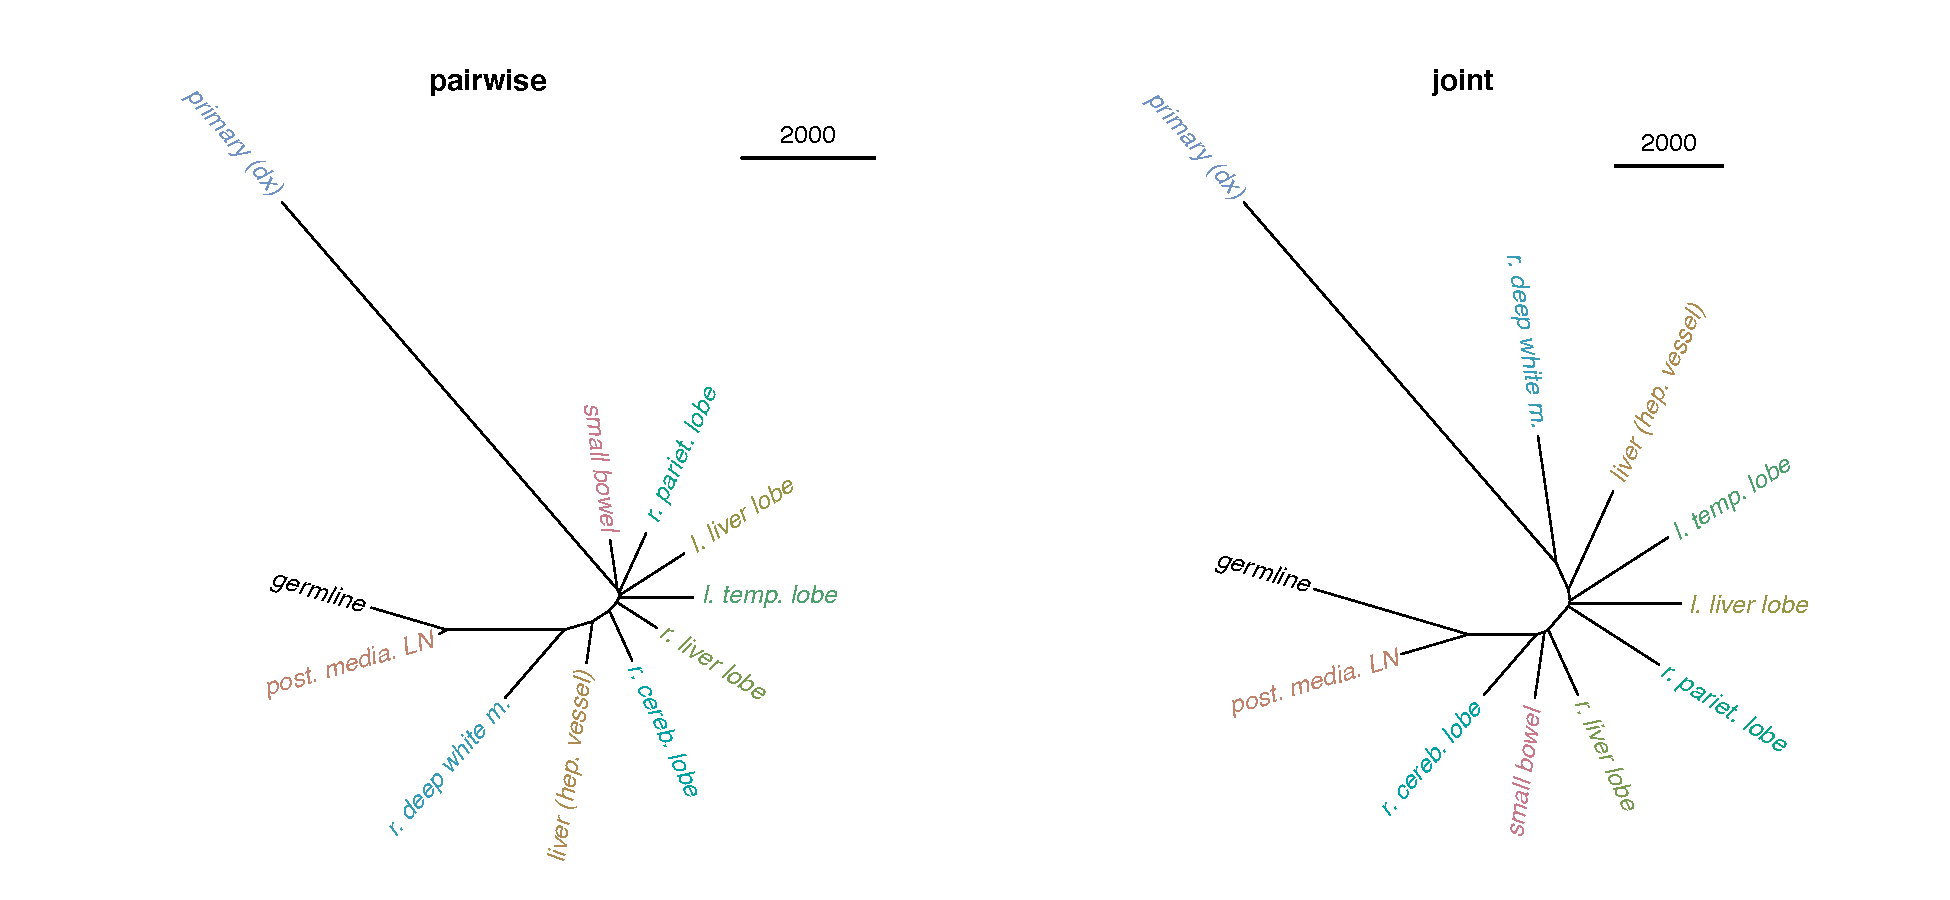
\includegraphics[width=.99\linewidth]{Figures/phyloCA9.pdf}
\caption[Reconstructed phylogenies of joint samples]{Reconstructed phylogenies of a patient with multiple spatially distinct samples; Neighbour joining on Hamming distance on variant occurrence vector. Tip labels describe the location of the sample in the patient. Trees are shown as unrooted with germline as fixated origin point; black line ruler shows the length of an edge with 2000 mutations}\label{fig:ca9phylo}
\end{figure}

\todo[inline, color=green]{Maybe adjust the font size in the trees to make it more readable}

There are several obvious changes, first in the longer edge connecting the germline to all other samples, which we consider as the state of no somatic variants. This shows that there are many more shared mutations in all samples, than what would have been anticipated with the default method, which corresponds to an overestimation of the heterogeneity of the samples. As the accumulation of somatic variants is still used as a proxy for timing and cell divisions, when assuming a high mutation rate for lung cancer ($5.3 \cdot 10^{-8}$ from \citeauthor*{Werner2020} \cite{Werner2020}) this difference of $\approx 36000$ variants is equivalent to $\approx 2000$ cell divisions. While the cell doubling rate of lung cancers is highly dependent on the type \cite{Arai1994}, this change makes a substantial difference when assessing the timing of the tumour initiation and further evolution. 

Secondly, there have been topological changes, which generate a longer bifuricating edge between the olive coloured ``r. liver lobe`` and the ``r. pariet. lobe`` showing a bottle neck in cancer evolution, which fits very well with the clinical history, where the patient lived with stable disease for almost ten years, before progressing and dying. The extreme distance of the primary/diagnostic sample from the rest of the samples could be either a difference in sequencing quality, or due to the exposure to FFPE for the ten years between tumour diagnosis and death. However, as this feature is preserved between both the joint and the pairwise analysis, it does not appear to be an effect of our new method.

\begin{figure}[!ht]
\centering
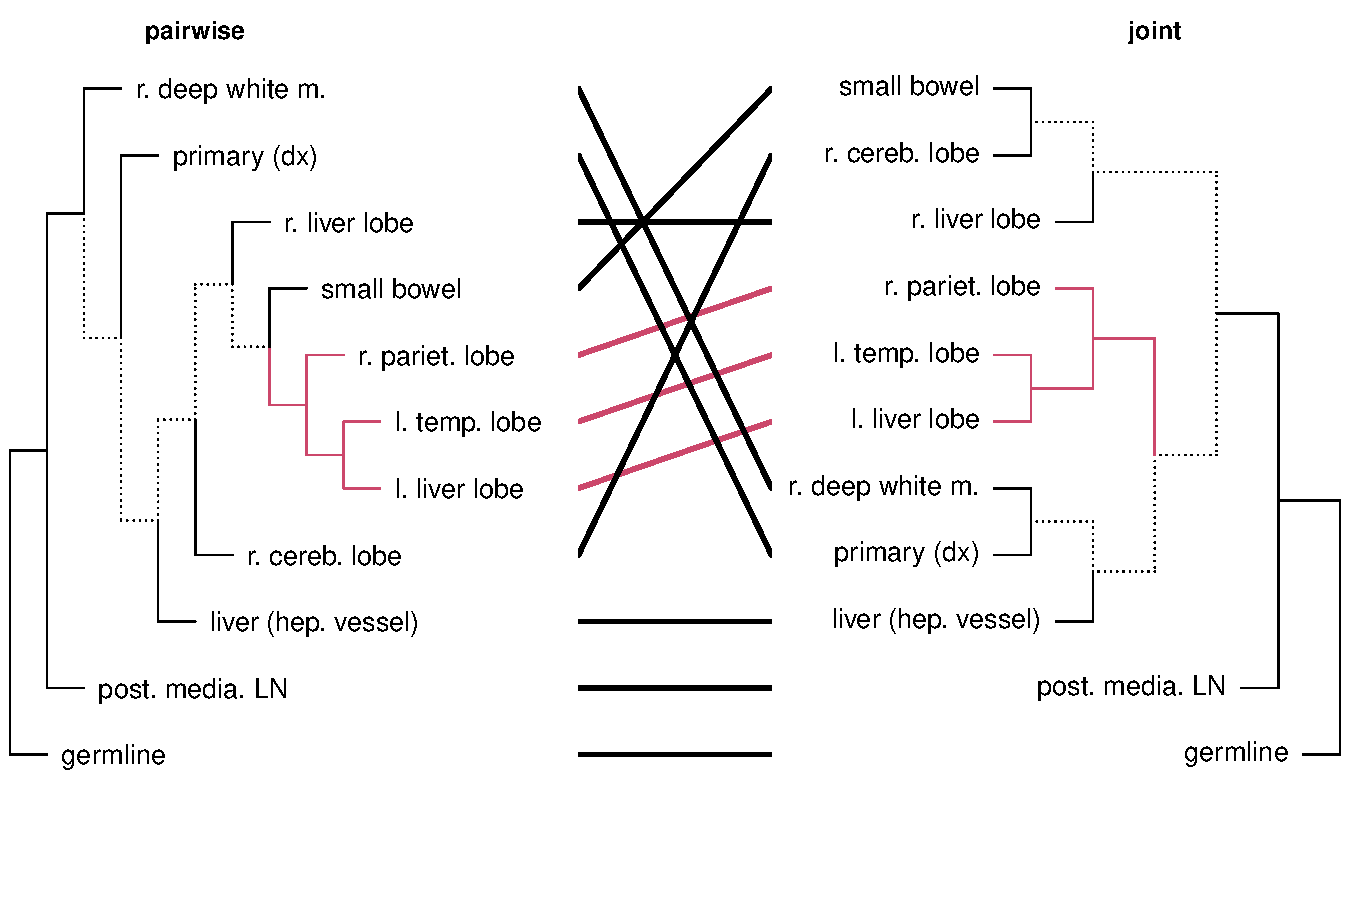
\includegraphics[width=.99\linewidth]{Figures/tanglePhyloCA9.pdf}
\caption[Tanglegram of the reconstructed phylogenies]{Side by side view of the reconstructed trees from \autoref{fig:ca9phylo}; internal edges, which are distinct between trees are shown as dotted lines; common subtree is shown in red  Tree labels have been sorted to minimise distance between labels; Visualisation generated with dendextend \cite{Galili2015}}\label{fig:tanglePhyloCA9}
\end{figure}
\todo[inline, color=green]{maybe increase the line width of the edges}

\autoref{fig:tanglePhyloCA9} shows a topology focused view of the two trees, which highlights the breaks which are needed to morph one tree into the other with dotted edges \cite{Vienne2018}. The common subtrees are coloured the same on both sides and connecting lines show identical labels. This format shows that while the trees look quite similar at first glance, they show vastly different topologies.


One example of this is ``small bowel`` which was connected to the red common subtree, but is now much closer to the ``r. cereb. lobe`` and forms a parallel clade with the ``r.liver lobe``. In general, where the pairwise tree shows a very linear topology, which leaves only branching out of the main with no disjunct subclades, which are clearly present in the joint reconstruction.  (\autoref{fig:tanglePhyloCA9}).


\section[Longitudinal analysis]{Longitudinal analysis}
\label{variantcalling-sec:longitudinal}

The initial motivation for the development of our workflows was the analysis of multi-region, or spatial, samples from the same patient coming from the CASCADE rapid autopsy program. However, we were very interested on applying the methods on longitudinal samples from patients, for example, for the joint analysis of diagnostic and relapse sample, or even the repeated testing of ctDNA are quite worth thinking about. In this part, I will present work using the published workflows on a longitudinal dataset, which highlights the flexibility and widespread usability of the new methods.

In addition to their autopsy which resected nine distinct metastatic sites, Patient ``CA-F`` also had three longitudinal blood samples taken, from which ctDNA was extracted and WES performed. These blood samples were taken as non-invasive surveillance seven, five and two months before the death of the patient (\autoref{fig:CA-Ftimeline}). In a study of late stage melanoma patients, \Citeauthor{Tan2019} identified ctDNA sequencing as a way to stratify patients into high and low risk of relapse and therefore inform adjuvant therapy \cite{Tan2019}. This makes patient ``CA-F`` a very good test dataset to showcase the improvement with joint variant calling. Similar to the spatially related samples, the joint analysis can improve the performance, which then in turn enable the detection of lower allele frequency variants, either through lower tumour burden or through the limited availability of DNA fragments from brain lesions due to the blood brain barrier \cite{2014}.

\begin{figure}[!ht]
\centering
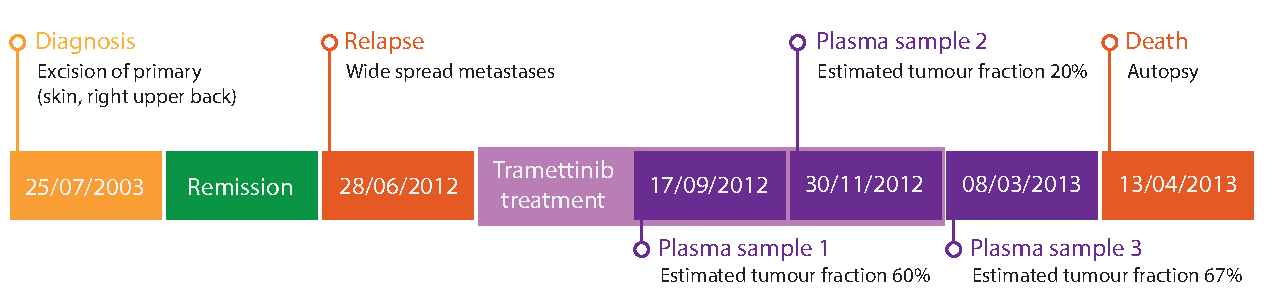
\includegraphics[width=.99\linewidth]{Figures/CA-F_timeline.pdf}
\caption[Timeline from diagnosis till death for patient CA-F]{Timeline from diagnosis till death for patient CA-F: 1.9mm melanoma removed after diagnosis \dateenglish\formatdate{25}{07}{2003} but with negative sentinel lymph node biopsy; \dateenglish\formatdate{28}{06}{2012}: PET scan and subsequent liver biopsy confirm relapse with wide spread metastases; trametinib treatment from Oct. 2012 till Jan. 2013 with minor response; blood plasma samples during treatment (1 and 2) as well as after progression (3); death and rapid autopsy of nine metastatic sites (\dateenglish\formatdate{13}{04}{2013})}\label{fig:CA-Ftimeline}
\end{figure}


To show that even in longitudinal data, the joint analysis can boost the signal, we jointly variant called the diagnostic biopsy sample with the three ctDNA samples and compared them with the results from the pairwise analysis. On average, we found 2905 additional variants in each of the ctDNA samples, which is more than doubles the average number of variants found with the pairwise analysis (2414). Out of those, we found 534 variants in the ctDNA samples, which were found as a high confidence variant in the diagnostic sample, indicating that these findings are high quality calls. 

\begin{figure}[!ht]
\centering
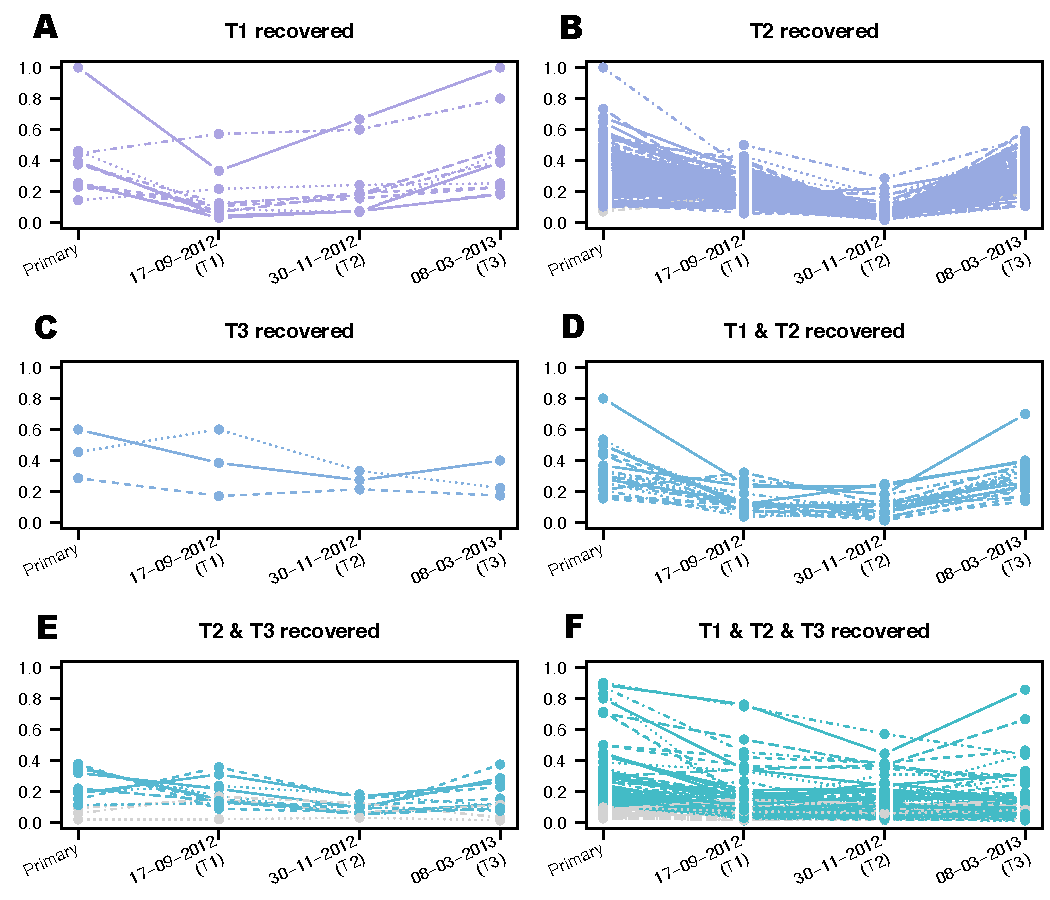
\includegraphics[width=.99\linewidth]{Figures/longitudinalCA9ctDNAVafs.pdf}
\caption[Improved somatic variant calling in longitudinal data]{Improved somatic variant calling in longitudinal data: Variant allele frequency (VAF) of variants found additionally through joint variant calling which were found as high confidence variants in the primary sample; Variants with less than 0.1 VAF in the primary are coloured grey; ``T1 recovered`` shows variants, which were high confidence in all ctDNA samples but T1 and were only found through joint calling there; Axis label show the date of blood collection }\label{fig:longitudinalVAFsctDNA}
\end{figure}

Exactly like in the spatially different samples, in longitudinal data lower tumour purity samples benefit more from the joint analysis. We see that time point 2 (T2) has the highest amount of recovered variants (377) which are found as high confidence variants in both other time points (\autoref{fig:longitudinalVAFsctDNA} A vs. B vs. C) and T2 also has the lowest tumour purity in the cfDNA recorded (T1: 60\%; T2: 20\%; T3: 60\%) however, there are still 106 variants, which were not found in the ctDNA samples at all with the pairwise analysis at all, even though they were high confidence variants in the primary sample (\autoref{fig:longitudinalVAFsctDNA}F). These variants usually show a lower depth of coverage (dp) in the ctDNA samples, which may possibly indicate a problematic region in the genome, but rather than it not being called a variant, it is just a sign of incomplete data, which can be used with our joint approach. 

\begin{figure}[!ht]
\centering
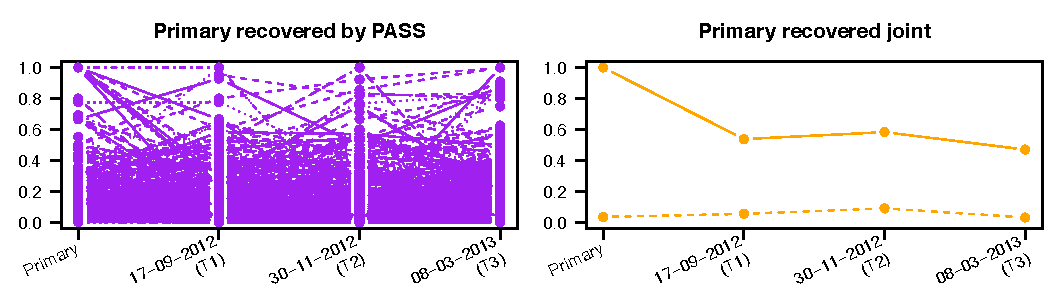
\includegraphics[width=.99\linewidth]{Figures/longitudinalCA9primaryVafs.pdf}
\caption[Longitudinal data informs diagnostic variant calling]{Longitudinal data informs diagnostic variant calling: Vafs of variants additionally found through joint calling in the primary samples; Primary recovered by PASS shows variants which were high confidence in at least one ctDNA sample; Primary recovered joint shows variant which were low confidence in all samples in the pairwise analysis; Axis label show the date of blood collection}\label{fig:longitudinalVAFsprimary}
\end{figure}


Finally, we can also find 398 additional variants in the   primary sample. 398 were discarded due to missing data in the tissue sequencing, but could be found with a high confidence in the longitudinal data and two of the variants were included, as all 4 samples had this variant below the detection threshold (\autoref{fig:longitudinalVAFsprimary}). The missing depth in the primary also leads to the occasional very high allele frequency of the variant, as all available reads show the variant, but their numbers are below the threshold normal variant callers will report variants.

This shows that both spatially and longitudinal related samples should be analysed jointly, as it substantially increases the amount of true variants found, which as shown before, can have a large impact on downstream analysis of the samples.



\subsection[Clonal deconvolution]{Clonal deconvolution}
\label{variantcalling-sec:clonal}

On of the most important information derived from multiple related samples from the same patient is the clonal deconvolution, where subclonal reoccurring patterns of mutations (clones) are resolved both spatially and longitudinally. These reoccurring clones can be linked to either parallel evolution through positive selection pressure, like a targeted drug, or to the process of developing metastases where a piece of the cancer ``breaks`` off and grows at a different site.
In contrast to the lack of options for joint somatic variant calling, there is a plethora of algorithms and methods available for clonal deconvolution. Since 2015 PhyloWGS \cite{Deshwar2015}, Canopy \cite{Jiang2016}, CLOE \cite{Marass2016}, CloneFinder \cite{Miura2018}, MACHINA \cite{ElKebir2018} and MOBSTER \cite{Caravagna2020} were published, to name a few. Underlying all these models is a form of clustering variants with similar variant allele frequency together, to reduce the combinatorial space and enhance the confidence in the signal \cite{Tarabichi2021}. Due to the high number of tools, it is very challenging to select the right tool, especially since all of them have advantages and disadvantages \cite{Miura2020}. In this work I decided to use PhylogicNDT \cite{Leshchiner2018} as it has been shown to work well on clinical samples \cite{Gerstung2020} and does not have the restriction for the input to be from copy number neutral areas which many of the other tools have.


Both the variants found with the default pairwise as well as with the new joint workflows were annotated with their local allele specific copy number to form a MAF like file format which is required by PhylogicNDT. While PhylogicNDT allows the user to supply the cancer cell fraction for every variant, the program can also estimate them from the supplied allelic counts and the copy number. Local copynumber calls were derived from copy number segment calls made by sequenza by intersecting chromosomal location of each variant with the copy number segment containing the variants location. This requires multiple steps and the source code is shown in \autoref{lst-jvcAppendix:parseVcf} (parsing VCF), \autoref{lst-jvcAppendix:cnv} and \autoref{lst-jvcAppendix:convertMAF} (convert to MAF format). Variants which couldnt be annotated with copy number information, because their genomic location did not overlap with any called copy number segment, were discarded for this analysis.

\begin{figure}[!ht]
\centering
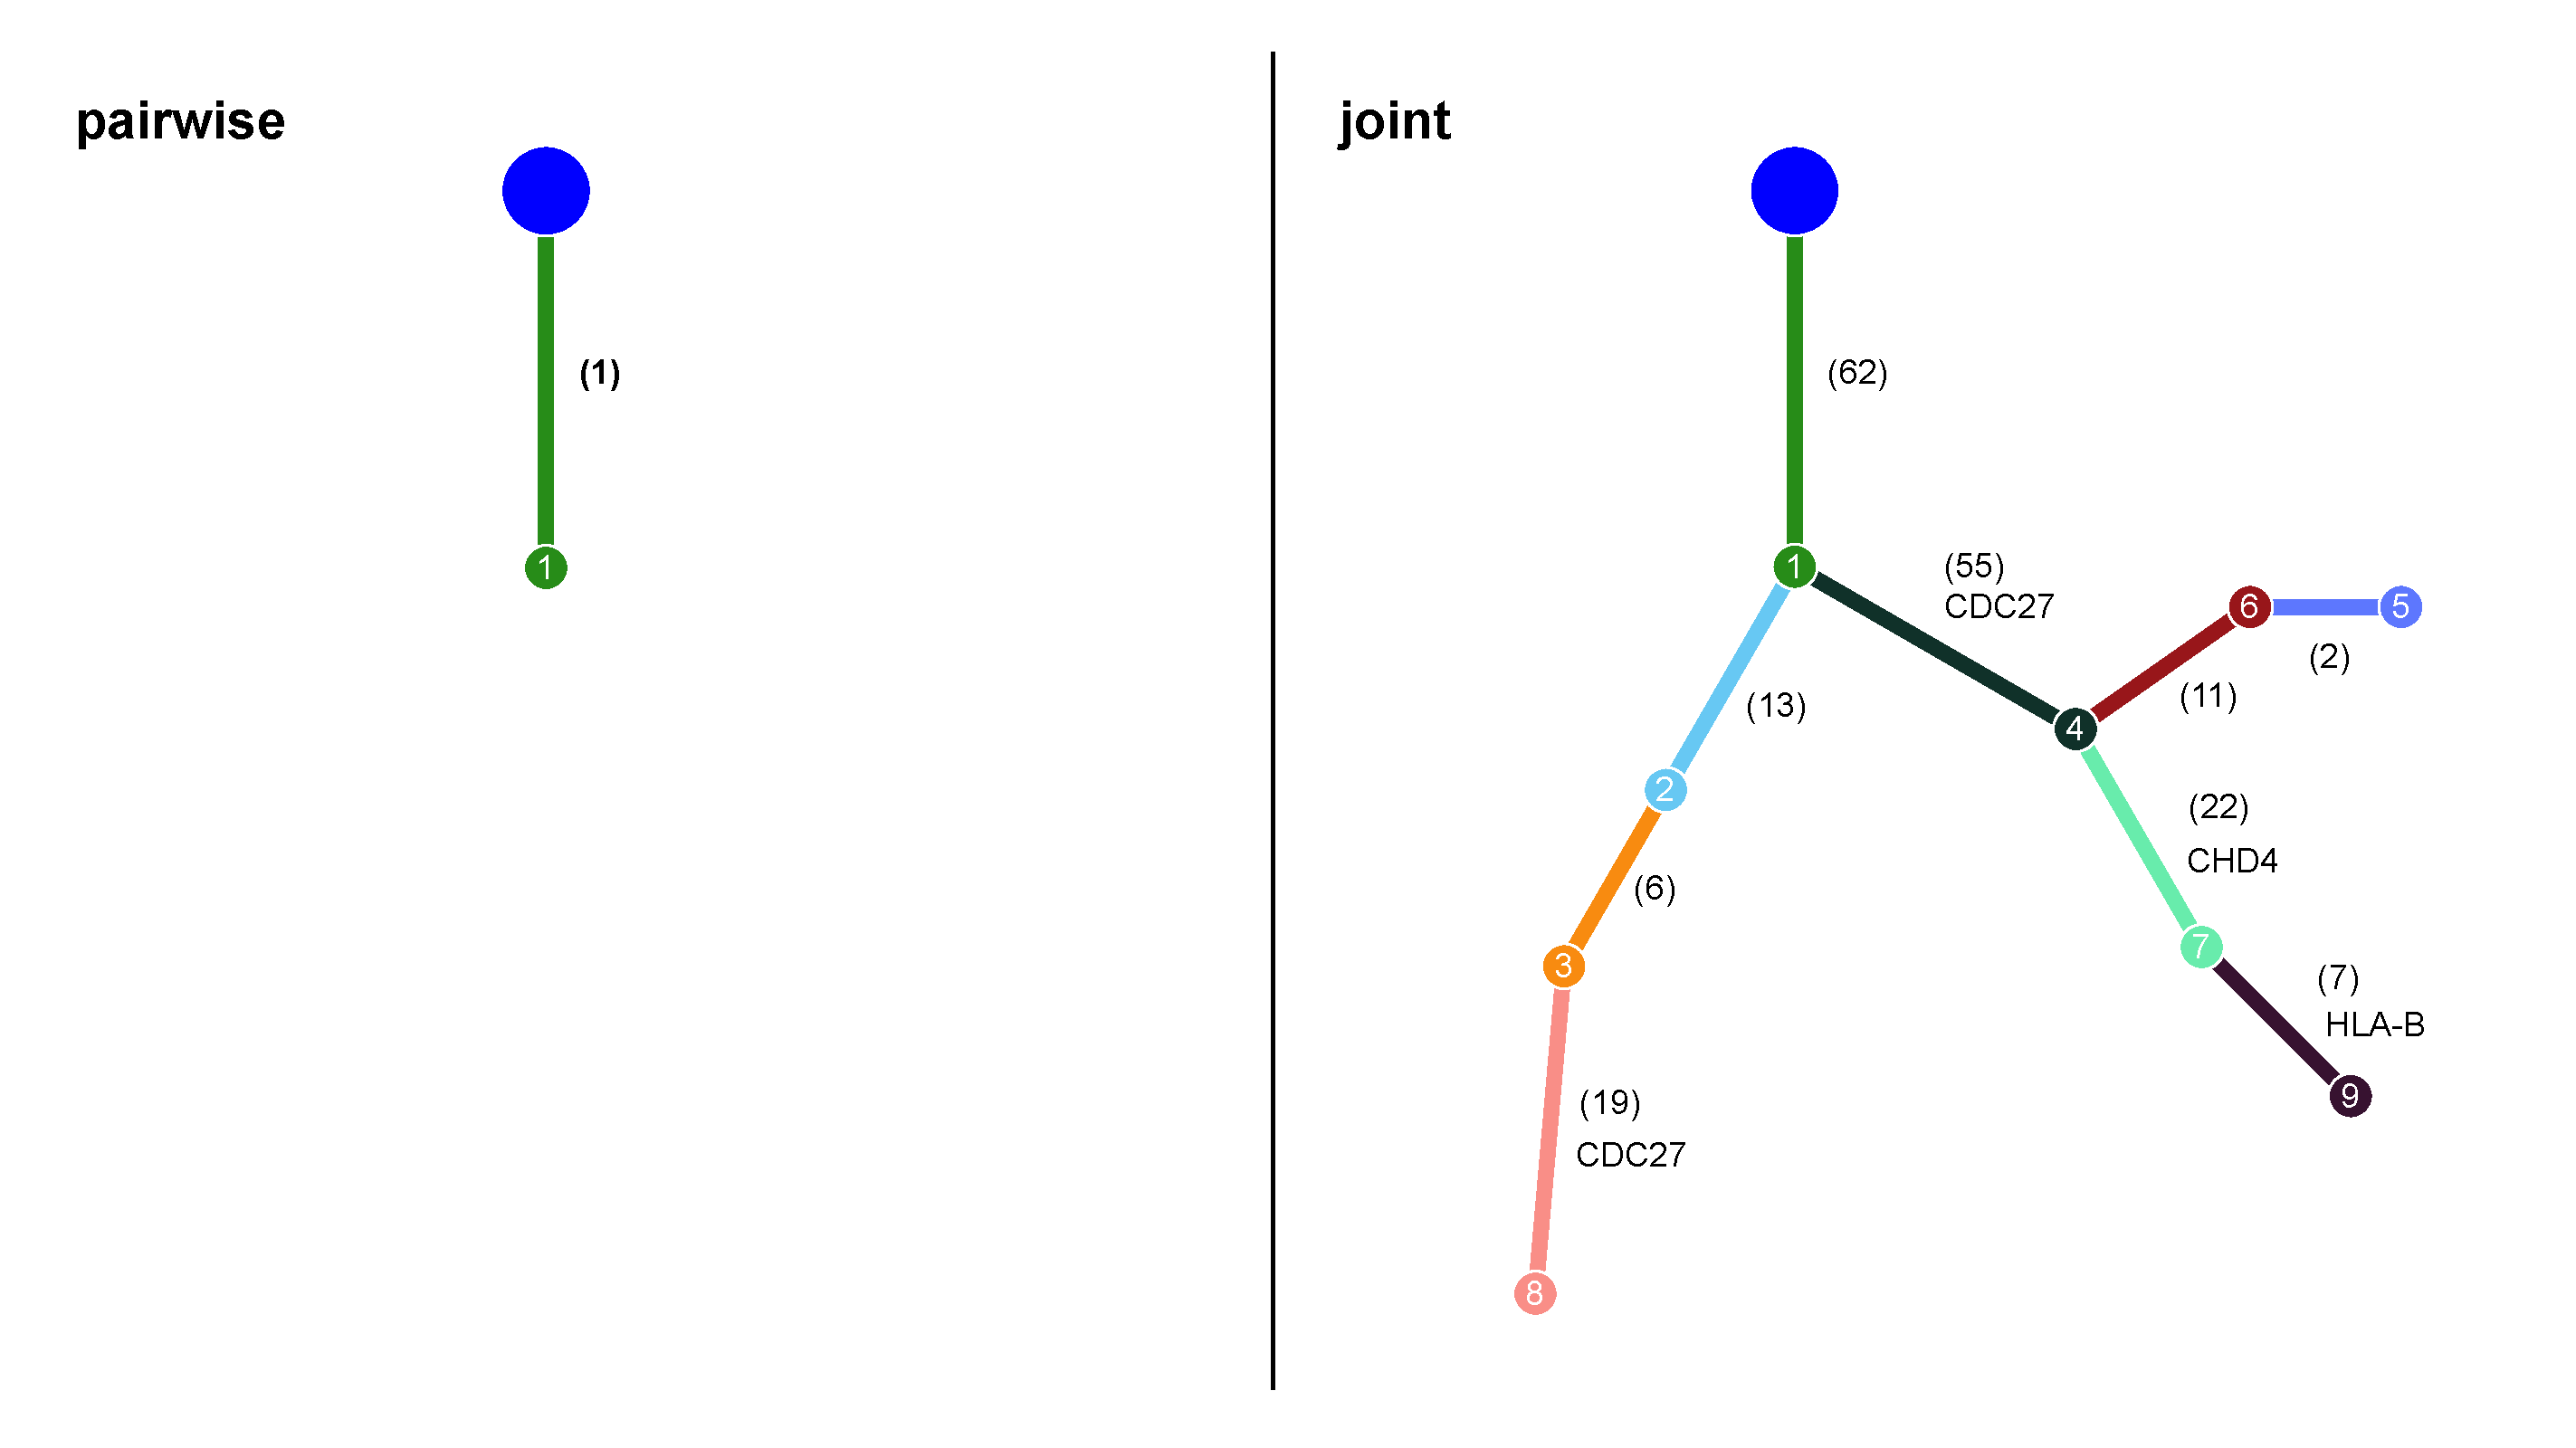
\includegraphics[width=.99\linewidth]{Figures/clonalDeconv.pdf}
\caption[Reconstructed clonal trees for joint and pairwise variant calling]{Reconstructed clonal trees from PhylogicNDT; Blue circle at top depicts the germline/normal state. The coloured edges with the same coloured circle represents a distinct subclone of the parent from which the edge emerges; The number in braces next to the edge is the number of mutations which define this subclone with an added gene symbol added, if there is a cancer driver gene mutation. The left part shows the result when using the default pairwise method of Strelka2 and the right side uses the results from the Strelka2Pass workflow}\label{fig:clonaldeconv}
\end{figure}


\autoref{fig:clonaldeconv} shows the highest parsimony clonal tree reconstructed by PhylogicNDT for the pairwise as well as the joint variant calling. As the copynumber calling information is the same for both inputs, the only difference is in the called variants. While there was no subclonal structure detected at all for the pairwise analysis, there is a highly variable structure detected using the jointly called variants. As this is a clinical sample, we cannot be certaine that the more branched model is the actual truth, but its biologically more logical that a late stage cancer has developed several subclones, rather than it being a very homogeneous disease at all of the 10 sites at autopsy with no evolution over ten years of disease \cite{Gerstung2020}.
It is of particular interest, that the \textit{CDC27} gene got mutated at different time points in different clones (clone 8 vs. clone 4), which a clear sign of parallel evolution, which would definitely be missed without the joint analysis.


\subsection{Longitudinal enriched phylogeny}
\label{variantcalling-sec:fullphylo}
Of course it is finally also possible to build a phylogeny with the spatial tissue samples and the longitudinal ctDNA samples. However, as the ctDNA give a holistic view of all cancer metastases (\autoref{intro-sec:ctDNA}) the interpretation needs to accommodate for that. 

\begin{figure}[!ht]
\centering
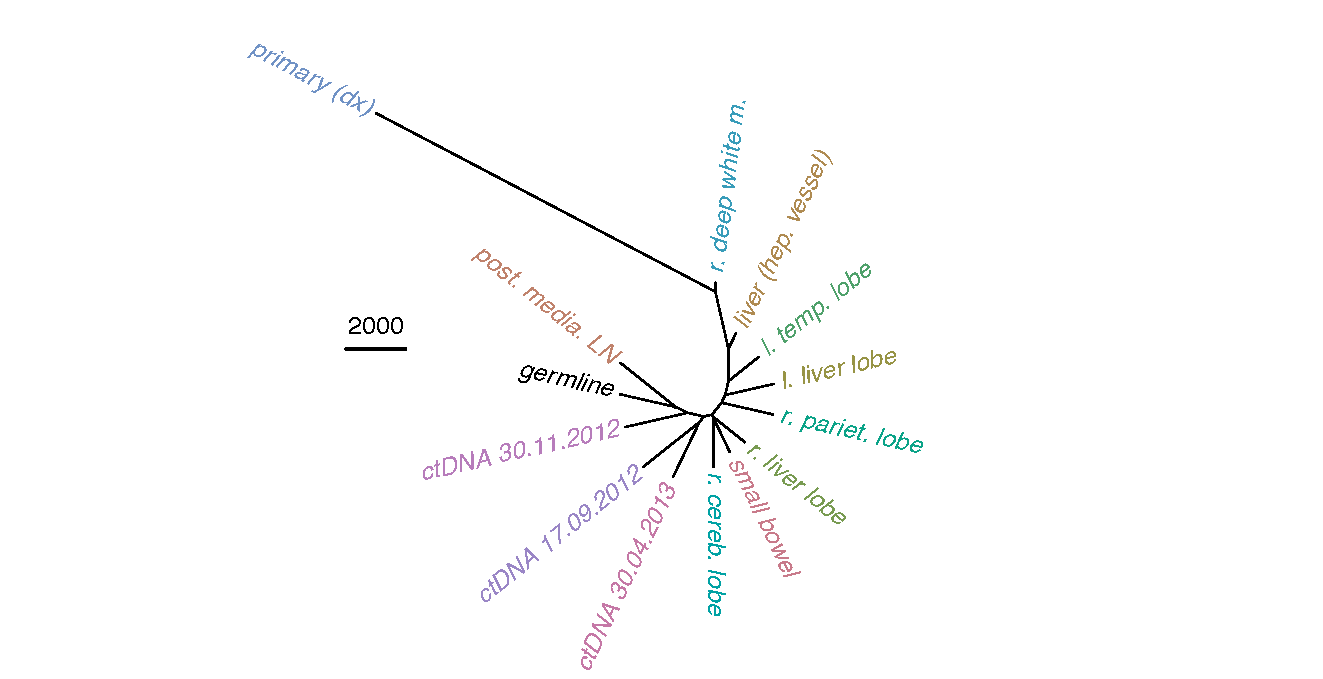
\includegraphics[width=.99\linewidth]{Figures/phyloCA9_withctDNA.pdf}
\caption[Reconstructed phylogeny with longitudinal ctDNA samples]{Reconstructed phylogeny with longitudinal ctDNA samples: Tree from \autoref{fig:ca9phylo} with three additional ctDNA samples from different time points about one year prior to death. The ruler shows the equivalent of 2000 mutations} \label{fig:phyloCA9ctDNA}
\end{figure}

The maybe most surprising thing is that the more temporally distant ctDNA samples from 17.09.2012 and 30.04.2013 are in a subclade together, away from the ``ctDNA 30.11.2012`` sample. Secondly, the addition of the ctDNA samples also lead to a further bipartition edge, which separates ``r. liver lobe``, ``small bowel`` and ``r. cereb. lobe`` from the rest of the tree (\autoref{fig:phyloCA9ctDNA}). This was already inferable from the topology of the previous tree in \autoref{fig:tanglePhyloCA9} ``joint``, but is even more pronounced with the inclusion of the ctDNA samples.

This shows that the addition of more samples helps to refine and improve the trajectory and history of cancer samples and it is vital to do this analysis jointly to generate the optimal result.

% usage of the tool
\section[Usage]{Usage statistics and uptake}
\label{variantcalling-sec:usage}
Ultimately when choosing research software, publication and citations are not a good metric to evaluate the quality of a method \cite{Gardner2022}. Many published software packages are not maintained or not even functional even though they are published. While we developed these joint somatic variant calling workflows to deal with a challenge we faced, the interest of others has been continuously expressed by bother members of the bioinformatics community  in the short period of time since publication.

\begin{figure}[!ht]
\centering
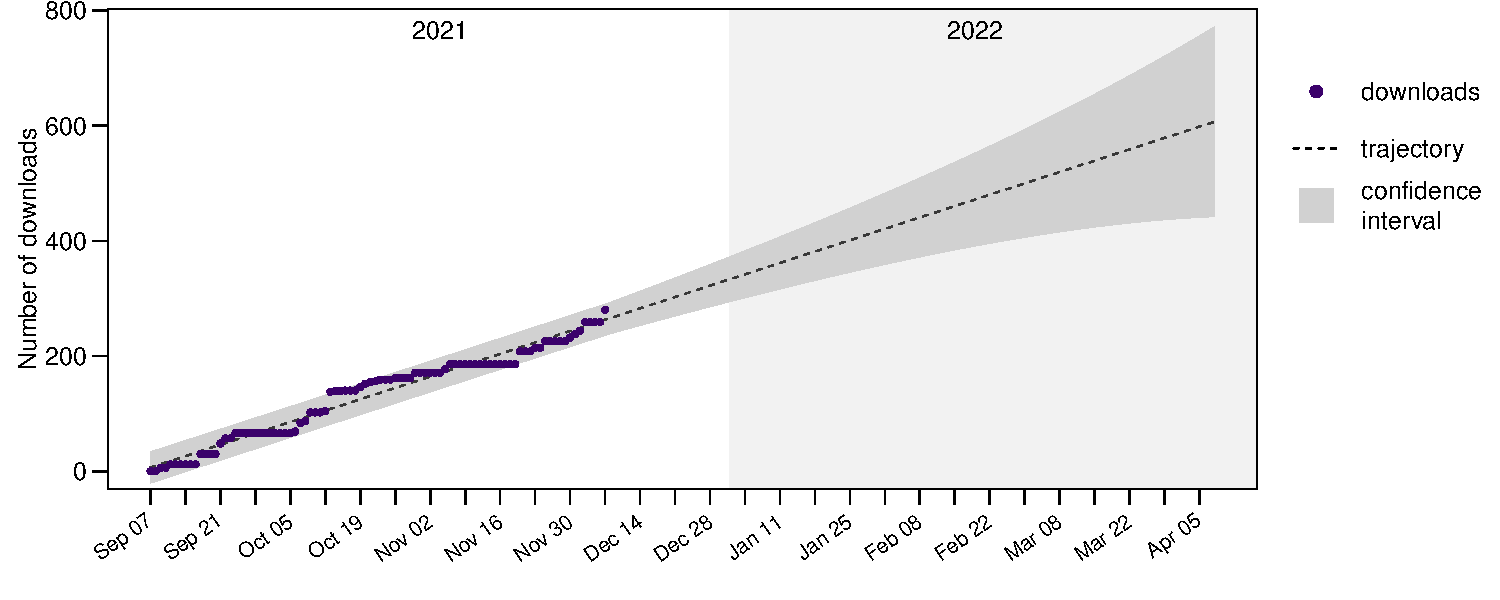
\includegraphics[width=.99\linewidth]{Figures/jointVariantCalling/dawsontoolkitDownloads.pdf}
\caption[Usage statistics joint workflows]{Cumulative download numbers of the ``dawsontoolkit`` docker container since publication of the manuscript; Actual counts are shown as dots, with smoothed trajectory depicted as dotted line with the 95\% confidence interval shown as a grey background; confidence interval has been adjusted with exponential decay of prediction accuracy with distance from the last data point; Start date 7$^{th}$ September 2021 (publication of method); End point prediction 31$^{th}$ December 2022 (End of current year); Numbers were recorded daily from the DockerHub API}\label{fig:usageStats}
\end{figure}

To have some proxy of the usage statistics of the workflows, we recorded the download numbers of the ``dawsontoolkit`` docker container after the publication of the manuscript. The container only consists of software for refiltering and joint analysis of the workflows . Obviously, this is an imperfect measurement, as people can reuse a downloaded container as often as they want, which would not appear in the count and similarly, just because the container was downloaded, the analysis might not have been used. Nevertheless, it still shows  an interaction and an interest in the methods. The download numbers show a sustained and stable increase in downloads (\autoref{fig:usageStats}). This suggests, that there is a need in the methods, rather than a simple curiosity after publication, which hopefully will facilitate a higher quality analysis of future projects and therefore lead to a better understanding of cancer evolution and heterogeneity.
  

% contains all the links for the cascade chapter

\begin{savequote}[85mm]
``Death is a release from and an end of all pains: beyond it our sufferings cannot extend: it restores us to the peaceful rest in which we lay before we were born``
\qauthor{--- Lucius Annaeus Seneca, \textit{De Consolatione ad Marciam}}
\end{savequote}

\chapter[CASCADE]{CASCADE - Late stage lung cancer in the spotlight}
\label{ch:cascade}
\addtocontents{equ}{\protect\addvspace{10pt}}

%\epigraph{``Death is a release from and an end of all pains: beyond it our sufferings cannot extend: it restores us to the peaceful rest in which we lay before we were born``}{--- \textup{Lucius Annaeus Seneca}, De Consolatione ad Marciam}

% intro for the chapter
\section{Introduction}
\label{cascade-sec:intro}

% the publication (maybe also Marian's publication)
\section{Publications}
\label{cascade-sec:publication}

This chapter includes and reproduces data analysis also shown in two publications, however due to the restriction of the university for sole first author, they are only mentioned here instead of included. 
The first publication features the resistance mechanism of small cell transformation (\textit{\citetitle{Burr2019}}~\textcite{Burr2019}) of one of the patients and the second shows the discovery of an emerging novel resistance to a targeted RET-fusion driven cancer (\textit{\citetitle{Solomon2020}}~\textcite{Solomon2020}).


% the analysis done as a total cohort
\section{Patient level analysis}
\label{cascade-sec:patientLevel}
In this section I will outline the work performed for each patient and highlight work specifically done for certain patients due to their unique clinical features. However most of the analysis is streamlined and the workflow applied the same way to each patient. The following sections expand on the individual steps.
\begin{enumerate}
\item \textbf{Quality control:} Each sample of a patient is checked for kinship and sequencing quality
\item \textbf{Read mapping}
\item \textbf{Joint somatic variant calling:} SNPs, InDels and SVs are called jointly
\item \textbf{Copy number calling}
\item \textbf{Variant effect annotation:} short and structural variants are annotated with possible biological effects
\item \textbf{Phylogenetic reconstruction}
\item \textbf{Clonal deconvolution}
\end{enumerate}

\subsection{Analysis workflow}
\label{cascade-sec:workflow}
This section summarises the primary analysis performed for each patient in detail. Specific analysis, like RNA analysis are discussed in the individual patient sections. 

\subsubsection{Quality control}
\label{cascade-sec:qc}
When multiple samples per patient are available, the possibility of sample mix-ups and issues is higher than when just dealing with a tumour normal pair, so in addition to the standard read depth, sequencing quality and reads-on-target analysis that is routinely performed after sequencing, we performed an additional step of kinship detection. We use concepts commonly employed in germline cohort analysis, like child and parents (trio) or even large databases (gnomAD). As most germline variants are due to mendelian inheritance, we can use the percentage of shared homo- and heterozygous germline variants to estimate the relatedness of two samples. For our analysis we used NGSCheckMate \cite{Lee2017} and all the results shown in later sections are based on it, however we also used Somalier \cite{Pedersen2020} on two patient samples with surprising kinship results but Somalier confirmed the result.

While this analysis is very useful to detect samples which do not belong to a patient, either through mislabelling or similar, it does not protect from mix-ups within a patients samples. However nothing but orthogonal validation will be able to discern these errors.

Other quality controls were performed with fastQC \cite{Andrews2010} for read integrity and \lq\emph{CollectWgsMetrics}\rq~from Picard \cite{Picard2018} for WGS samples and \lq\emph{samtools flagstat}\rq~\cite{Danecek2021} for on-target estimation for WES samples.

\subsubsection{Read mapping}
\label{cascade-sec:mapping}
For highest mapping performance, reads were aligned alternative contig aware with BWA~\cite{Li2013} (v0.7.17)  to GRCh38 (\emph{GCA\_000001405.15}) with alternative contigs but no decoy regions. Initial mapping was post-processed with \lq\emph{bwa-postalt.js}\rq~from bwa-kit to adjust the mapping assignment and quality mapping both to alternative and canonical contigs. Finally reads were duplicate marked with \lq\emph{MarkDuplicates}\rq~from the Picard-toolkit.

\subsubsection{Joint somatic variant calling}
\label{cascade-sec:jsvc}
For short variants (SNPs and InDels), the workflows presented in \autoref{ch:variantcalling} were used and while the Strelka2Pass workflow generates structural variants calls, they are not jointly called over all samples. Instead for the structural variants (SVs) we used GRIDSS2 \cite{Cameron2021}, which has a calling model for multiple related tumour samples and as GRIDSS2 is also a prerequisite for copy number calling with PURPLE (\autoref{cascade-sec:cnv}) using the same structural variants allows a higher conformity of analysis.


\subsubsection{Copy number analysis}
\label{cascade-sec:cnv}
After somatic variant calling, copy number analysis is a stable when dissecting the resistance and driver alterations of a tumour sample. While lung cancers are known for their high mutational burden \cite{Alexandrov2020}, often genetic amplifications can be found as driver or resistance mechanism. One of the more common resistance mechanisms is a high \textit{EGFR} or \textit{MET} amplification which significantly affect transcription \cite{Bjaanaes2021}. And while copy number alterations are often shared between metastases \cite{Ni2013}, the same heterogeneity that can be found in variant calling analysis also affects copy number analysis. Many modern copy number calling method will use the B-allele frequency , the allele frequency of a heterozygous germline variant, to gain allele specific copy number calls \cite{Favero2015,Talevich2016,Cameron2019a}. However each of those methods will only use the input of one tumour and one germline sample, very similar to \autoref{ch:variantcalling} we can actually improve the performance by analysing all tumour samples jointly. So far only HATCHet \cite{Zaccaria2020} has a joint copy number calling method.

\todo[inline]{Explain why we didnt use hatchet in the end? subjective parameter tuning?}
\todo[inline]{Explain purple vs sequenza for WGS vs WES}

\subsubsection{Variant effect annotation}
\label{cascade-sec:vep}
For small variants (SNPs and InDels) ``Variant Effect Predictor`` (VEP) version 92 \cite{McLaren2016} was used to assign possible effects. As a variant can affect multiple genes due to overlapping gene boundaries, effects within a curated list of lung cancer related genes (\autoref{A:cas:tab:lungcancergenes}) were assign an \lq\emph{IMPACT}\rq~ of \lq\emph{HIGHEST}\rq~ in order with the VEP provided impact values of \lq\emph{LOW}\rq, \lq\emph{MODERATE}\rq~ and \lq\emph{HIGH}\rq~. To only have one effect per variant, only the variant with the highest impact was returned. In case of multiple transcripts being affected with the same impact level, the putative canonical transcript result is used.

For structural variants, the effect annotation depends on the type of the structural variants. For amplifications and deletions, the genes within the variant are compiled and returned as a list. The effect of inversions and similar structural changes are assumed to be fusion based, so the breakpoint is annotated with the gene hit by both breakpoints and a potential fusion gene is returned.

\todo[color=green,inline]{potentially add the code for the effect annotation}

\subsubsection{Phylogenetic reconstruction}
\label{cascade-sec:phylo}

\subsubsection{Clonal deconvolution}

Clonal deconvolution for each patient was done with PhylogicNDT. To ensure high quality reconstruction, variants were filtered if the depth of coverage is lower than 8. All other called variants were transformed into the input format required in R. Cancer cell fractions (CCF) were left to PhylogicNDT with the option \lq\emph{--maf\_input\_type calc\_ccf}\rq~ by supplying the allele specific local copy number call for each variant the same way as shown in \autoref{variantcalling-sec:clonal} with the copy number calls from \autoref{cascade-sec:cnv}.

\subsection{Patient CA-A}
\label{cascade-sec:CA99}

This patient was a 61 year old male  with a metastatic \textit{RET-KIF5B} fusion positive NSCLC. After failure of Carboplatin, Pemetrexed, and Pembrolizumab as well as Lenvatinib, with compassionate access to Selpercatinib (\autoref{fig:ca99timeline}) he experienced almost immediate improvement with decreased levels of carcinoembryonic antigen and almost 100\% reduction of fusion positive ctDNA after one month (\autoref{fig:ca99ctDNA}). Similar to the ctDNA analysis, Positron emission tomography-computed tomography imaging revealed significantly reduced tracer uptake in multiple sites and partial response (\autoref{fig:ca99pet}).

\begin{figure}[!ht]
\centering
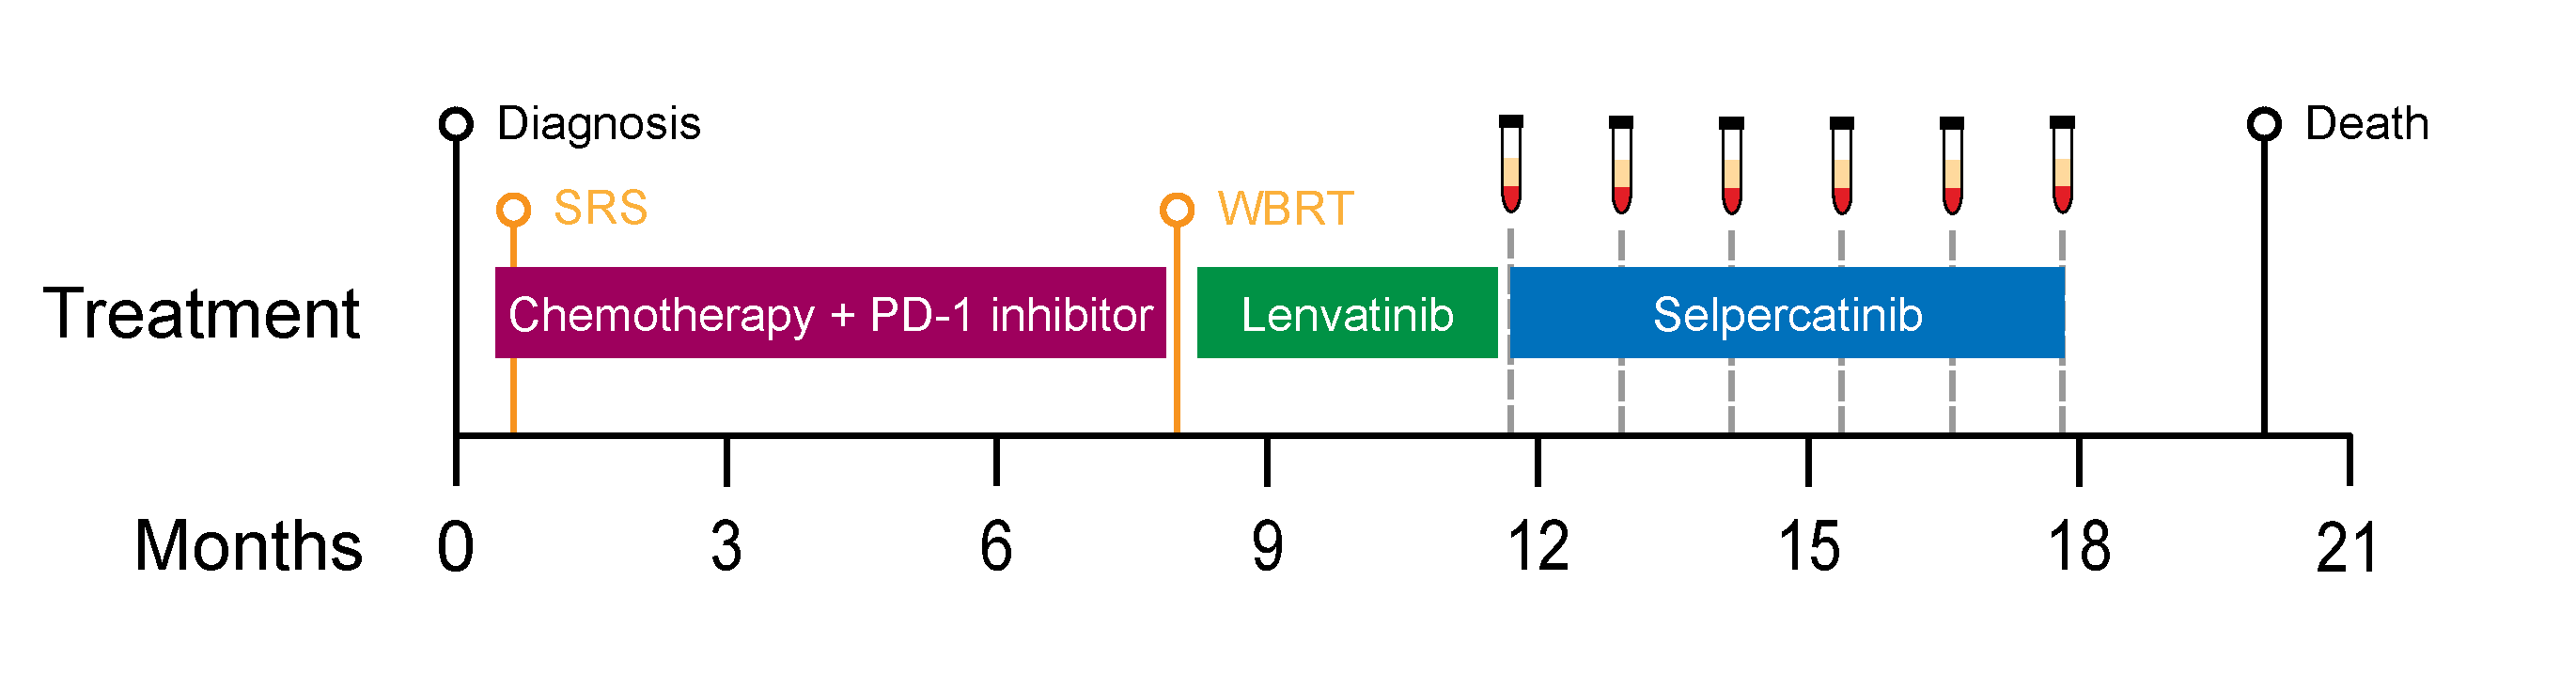
\includegraphics[width=.99\linewidth]{Figures/CA-A_timeline}
\caption[Timeline of patient CA-A from diagnosis until death]{Timeline of patient CA-A from diagnosis until death: Diagnostic biopsy detected \textit{KIF5B-RET} positive lung adenocarcinoma; SRS: stereotactic radiosurgery; WRBT: whole brain radiation therapy; a total of six blood samples were taken just before and during the selpercatinib treatment.} \label{fig:ca99timeline}
\end{figure}


Serial sampling of the plasma of the patient and analysis with the commercial Guardant360 assay \cite{Talasaz2014} revealed the previously undetected RET~G810S resistance mutation after three months of treatment . While at this point the driver mutation allele frequency was still dropping in the plasma, by month four the abundance of RET~G810S had increased and was accompanied by additional mutations in the same site (RET~G810R, C and V). In addition with the increase of fusion positive ctDNA this suggests that any mutation in this site affects the efficiency of Selpercatinib. While the patient initially was responsive to the treatment, repeat PET scans showed a progressive disease after six months, which ultimately lead to the death of the patient (\autoref{fig:ca99pet}).

\begin{figure}[!ht]
\centering
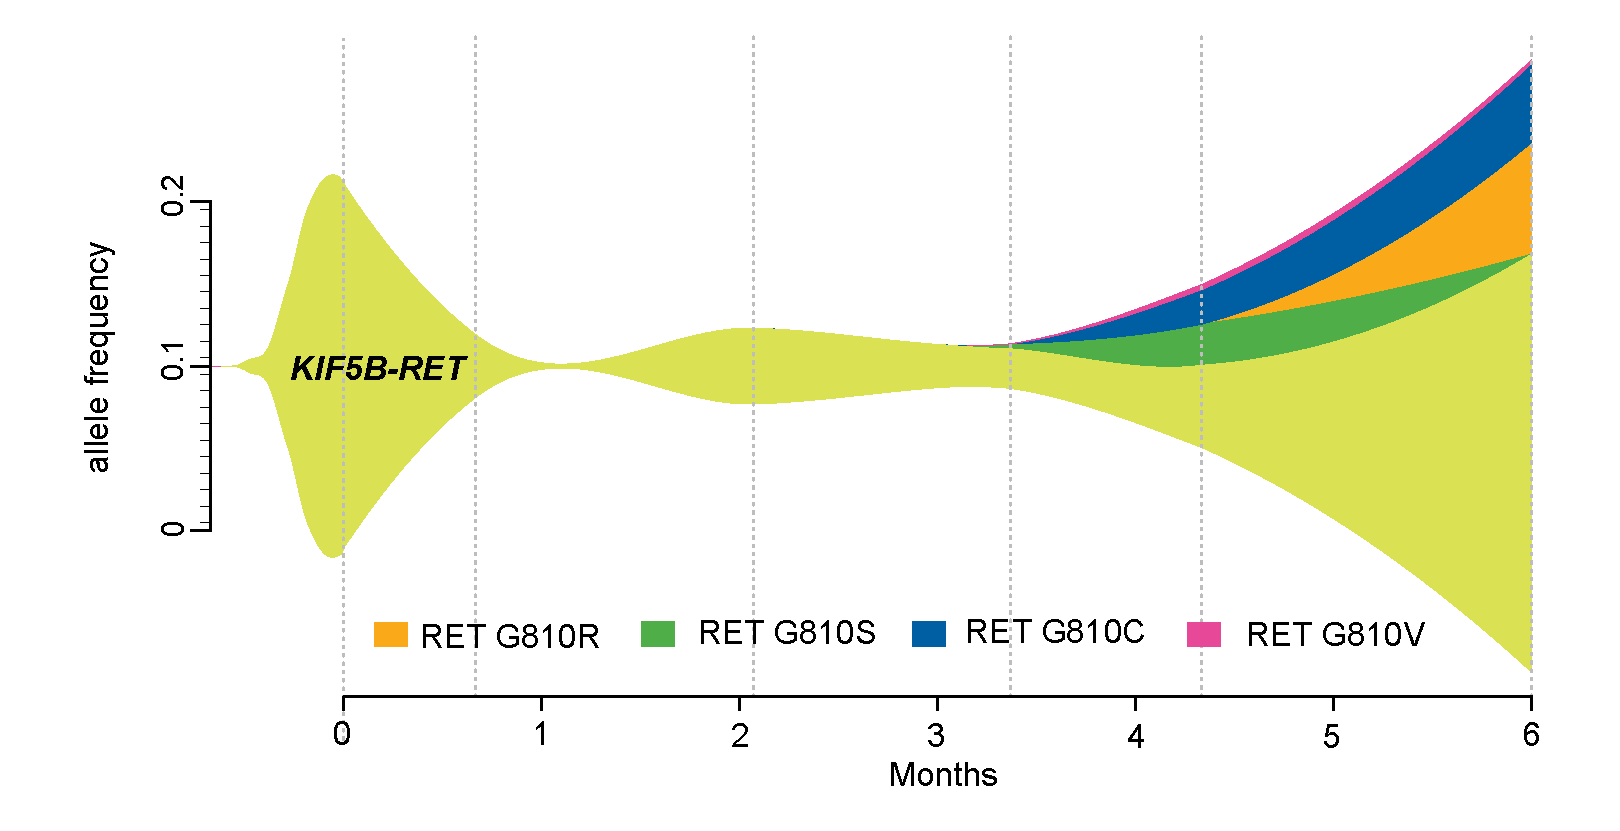
\includegraphics[width=.99\linewidth]{Figures/CA-A_ctDNAstream}
\caption[Allelic frequencies of of driver and emerging resistance mutations]{Allelic frequencies of of driver and emerging resistance mutations during Selpercatinib treatment (11 months after diagnosis); \textit{KIF5B-RET} fusion is the initiating driver with RET~G810R/S/C/V the emerging resistance SNPs} \label{fig:ca99ctDNA}
\end{figure}


\begin{figure}[!ht]
\centering
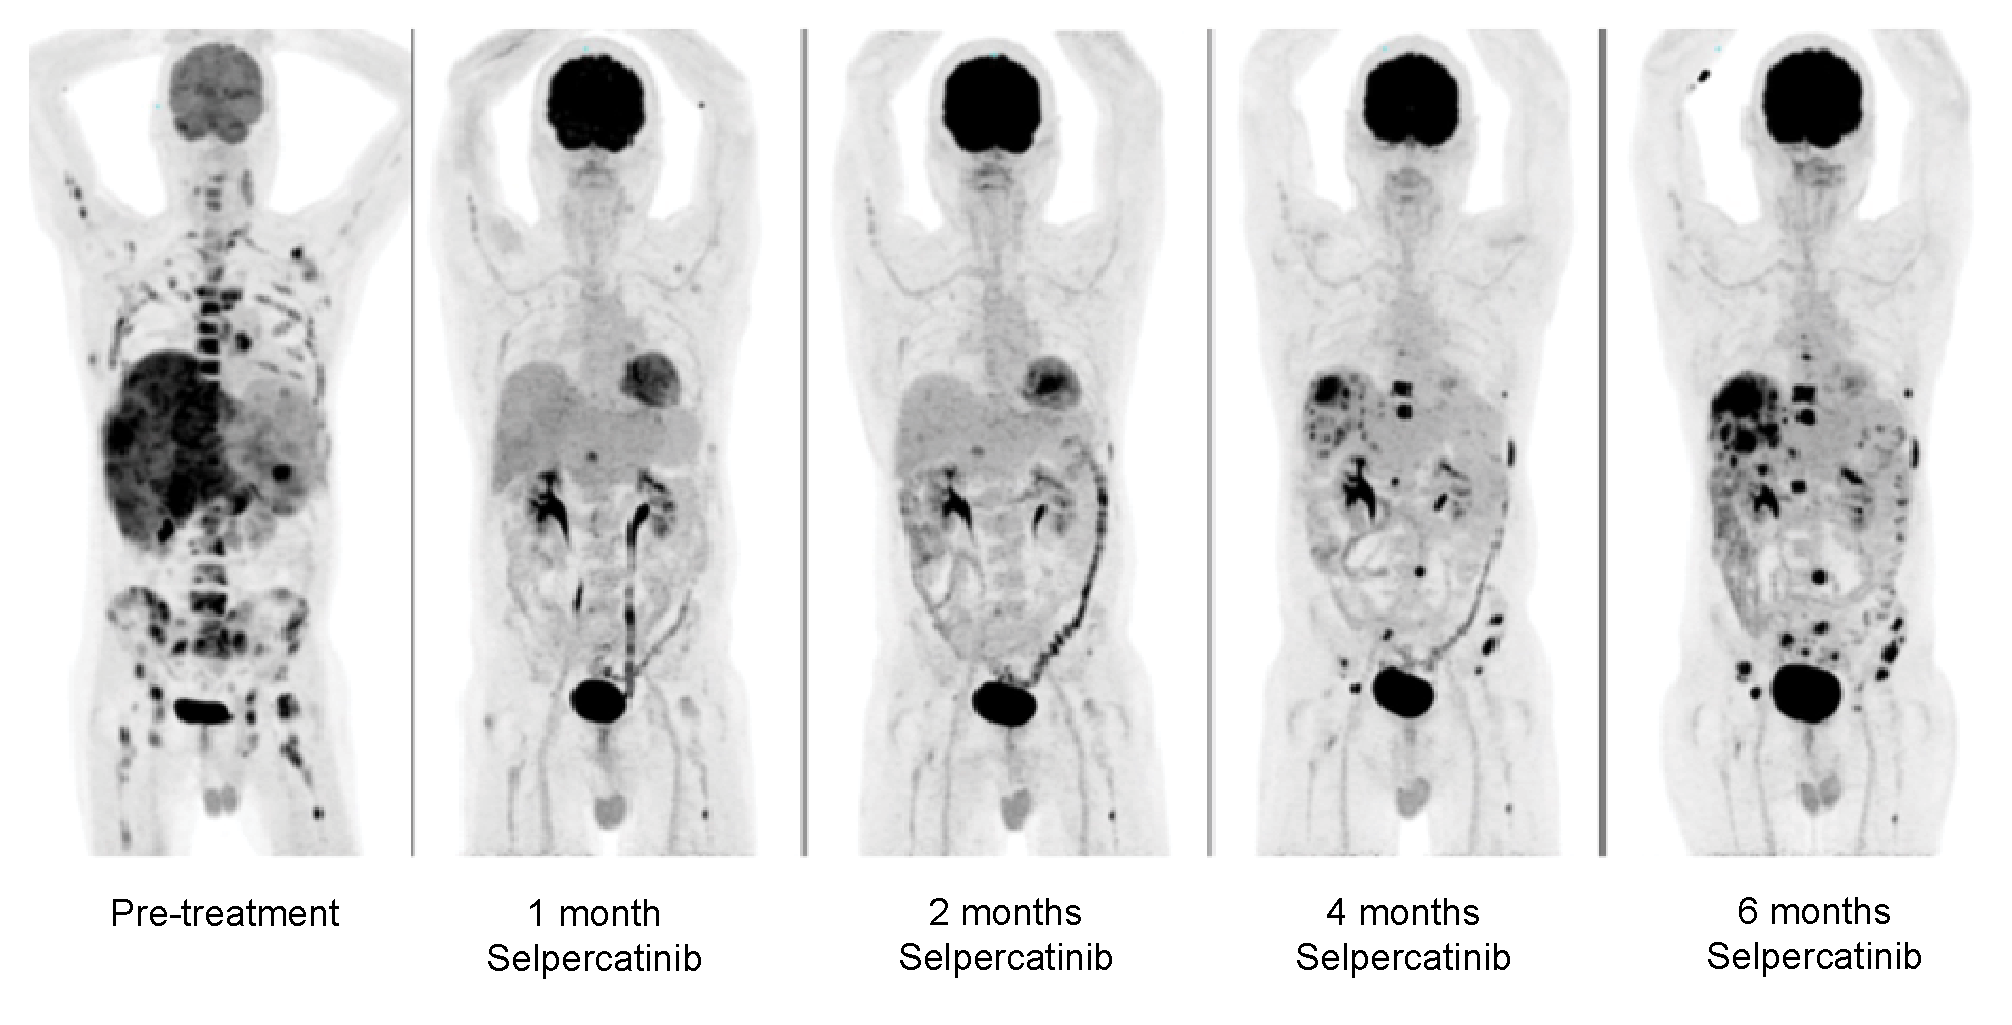
\includegraphics[width=.99\linewidth]{Figures/CA-A_PETscans}
\caption[PET scans of patient CA-A before and during Selpercatinib treatment]{PET scans of patient CA-A before and during Selpercatinib treatment} \label{fig:ca99pet}
\end{figure}


\begin{figure}[!ht]
\centering
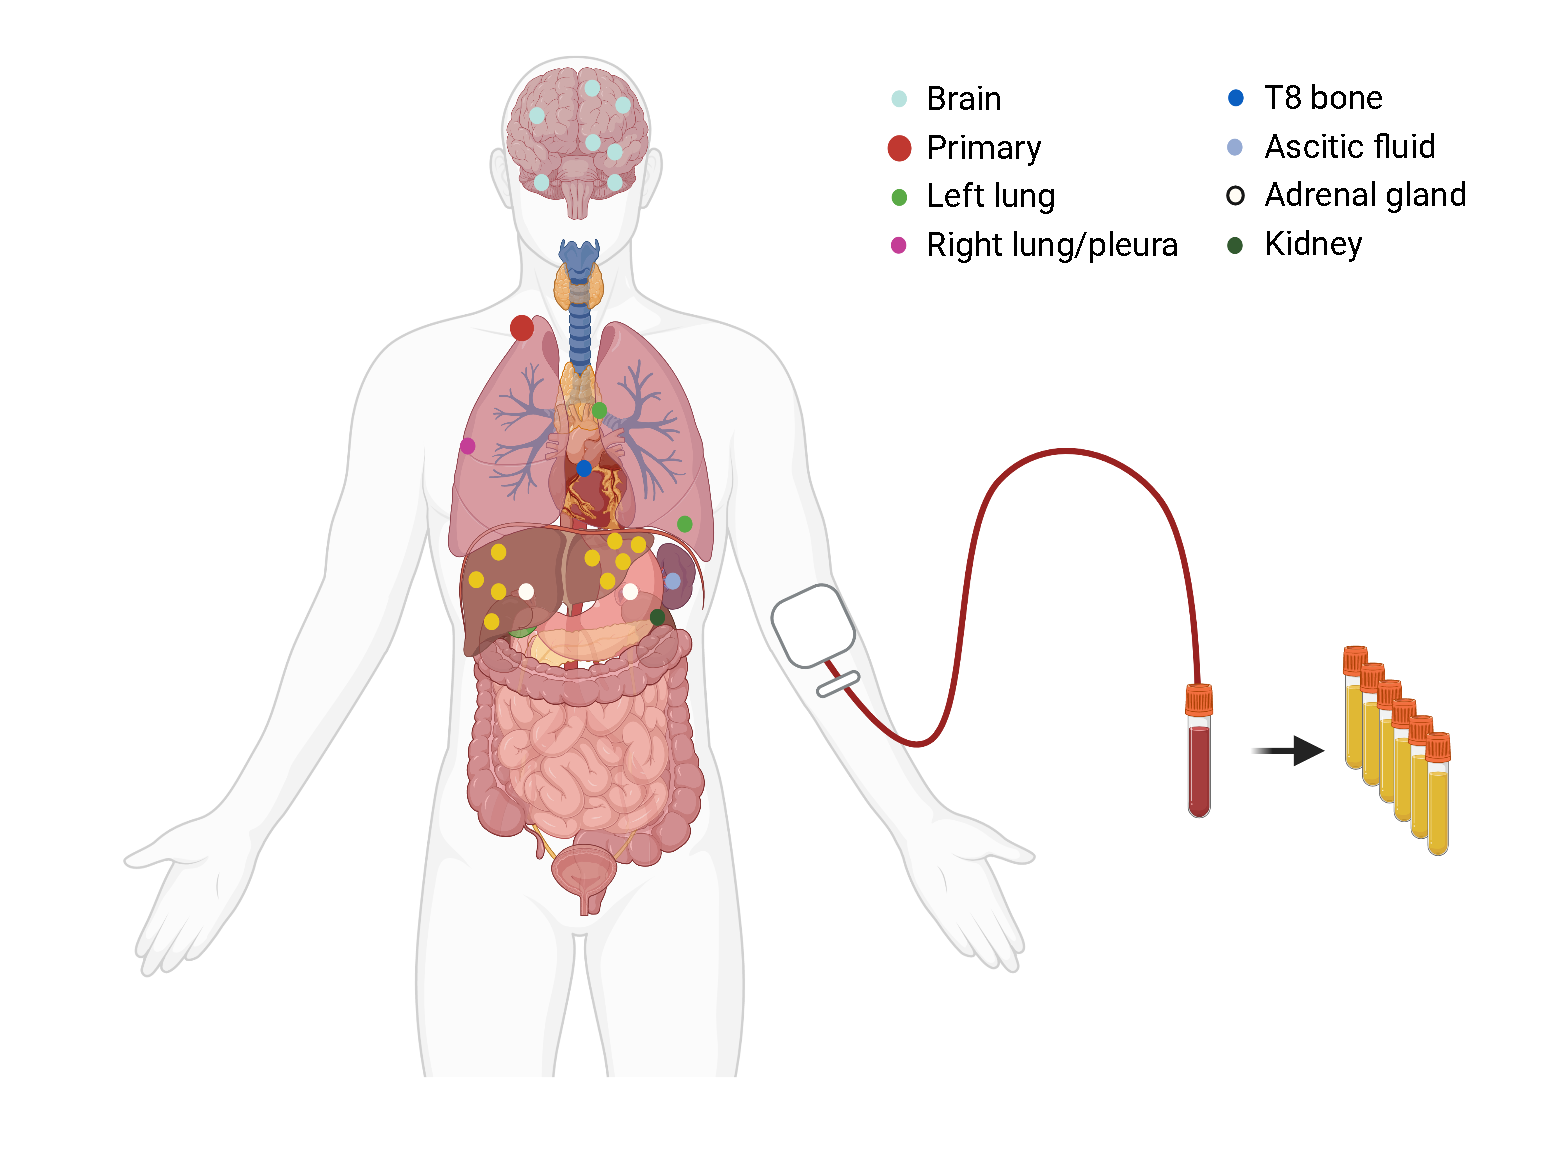
\includegraphics[width=.99\linewidth]{Figures/CA-A_schematic_CA99_organColours}
\caption[Schematic of tumour lesions in patient CA-A]{Schematic of tumour lesions in patient CA-A: Primary diagnostic sample shown in red; All 24 autopsy samples were coloured by organ they were collected from: Brain (7), left lung (2), right lung (1), liver (9), T8 bone (1), ascitic fluid (1), adrenal gland (2), kidney (1); Additionally to the post mortem blood sample, six serial blood samples were taken (\protect\autoref{fig:ca99timeline})} \label{fig:ca99schematic}
\end{figure}


At autopsy, 24 tumour tissue biopsies and a post mortem blood sample were collected and eight of them were selected for WGS at 130x coverage (\autoref{fig:ca99schematic}, \autoref{tab:ca99wgsSamples}\todo{add that info or remove the column}) and analysed with the standard workflow (\autoref{cascade-sec:workflow}).

\begin{table}
\caption[Autopsy samples sequenced for patient CA-A]{Autopsy samples sequenced for patient CA-A: Sample number is the internal sample collection during CASCADE autopsy, the organ of the sample, the fraction of tumour cell from H\& E stain and the pathology of the tumour sample.}\label{tab:ca99wgsSamples}
\centering
\rowcolors{2}{gray!15}{white}
\begin{tabular}{|c|c|c|c|c|}
\toprule
\hline
 \rowcolor{gray!50}
\textbf{Sample number} & \textbf{Organ} & \textbf{H \& E} & \textbf{Type}\\
\hline
 11 & right occipital lobe & 0.75 &  \cellcolor{white}\\
 26 & right liver lobe & 0.6 & \cellcolor{white} \\
 31 & left lower lung & 0.2 & \cellcolor{white} \\
 41 & left liver lobe & 0.2 & \cellcolor{white} \\
 47 & left liver lobe & 0.5 & \cellcolor{white} \\
 55 & left liver lobe & 0.4 & \cellcolor{white} \\
 57 & right liver lobe & 0.6 & \cellcolor{white} \\
 59 & right pleura & 0.7 & \cellcolor{white}\multirow{-8}{*}{lung adenocarcinoma} \\
 \hline
\bottomrule
\end{tabular}
\end{table} 

Somatic variant calling revealed substantial spatial heterogeneity, where both the occipital and the right pleura sample only contained RET~G810S, the right liver lobe harboured predominantly RET~G810R with either G810S and G810C as minor clones and lastly, the left liver samples showed almost even mix between G810C and G810S clones but no G810R presence \todo{do i need a figure here, like in the paper?}. The emergence of these mutations in multiple different sites at different allele frequencies, especially in already established sites in the liver, suggests that these mutations are the result of parallel evolution under positive selection through therapy, rather than seeding from one resistant clone.
Apart from the mutations changing RET~G810 no other variants affecting \textit{RET} or any other lung cancer genes were found in multiple samples. The occipital sample also contained a BRCA1~V939A  mutation and one left liver sample (47) showed a synonymous KIT~S967\%3D mutation. Additionally, no other variant found in non cancer related genes allowed the same explanation of resistance

The structural variant calling with GRIDSS showed consistent presence of the \textit{KIF5B-RET} fusion at high allele frequency (min: 0.27 max: 0.535), consistent with cancer cell fraction of 1 when correcting for local copy number changes  (min: 2 max: 3\todo{do i put a table or a figure here?}), in all but sample 31, which might be due to the low purity of the sample (\autoref{tab:ca99wgsSamples})

%we clear all floats before we go to the next patient
\cleardoublepage

\subsection{Patient CA-I}
\label{cascade-sec:CA51}



\begin{figure}[!ht]
\centering
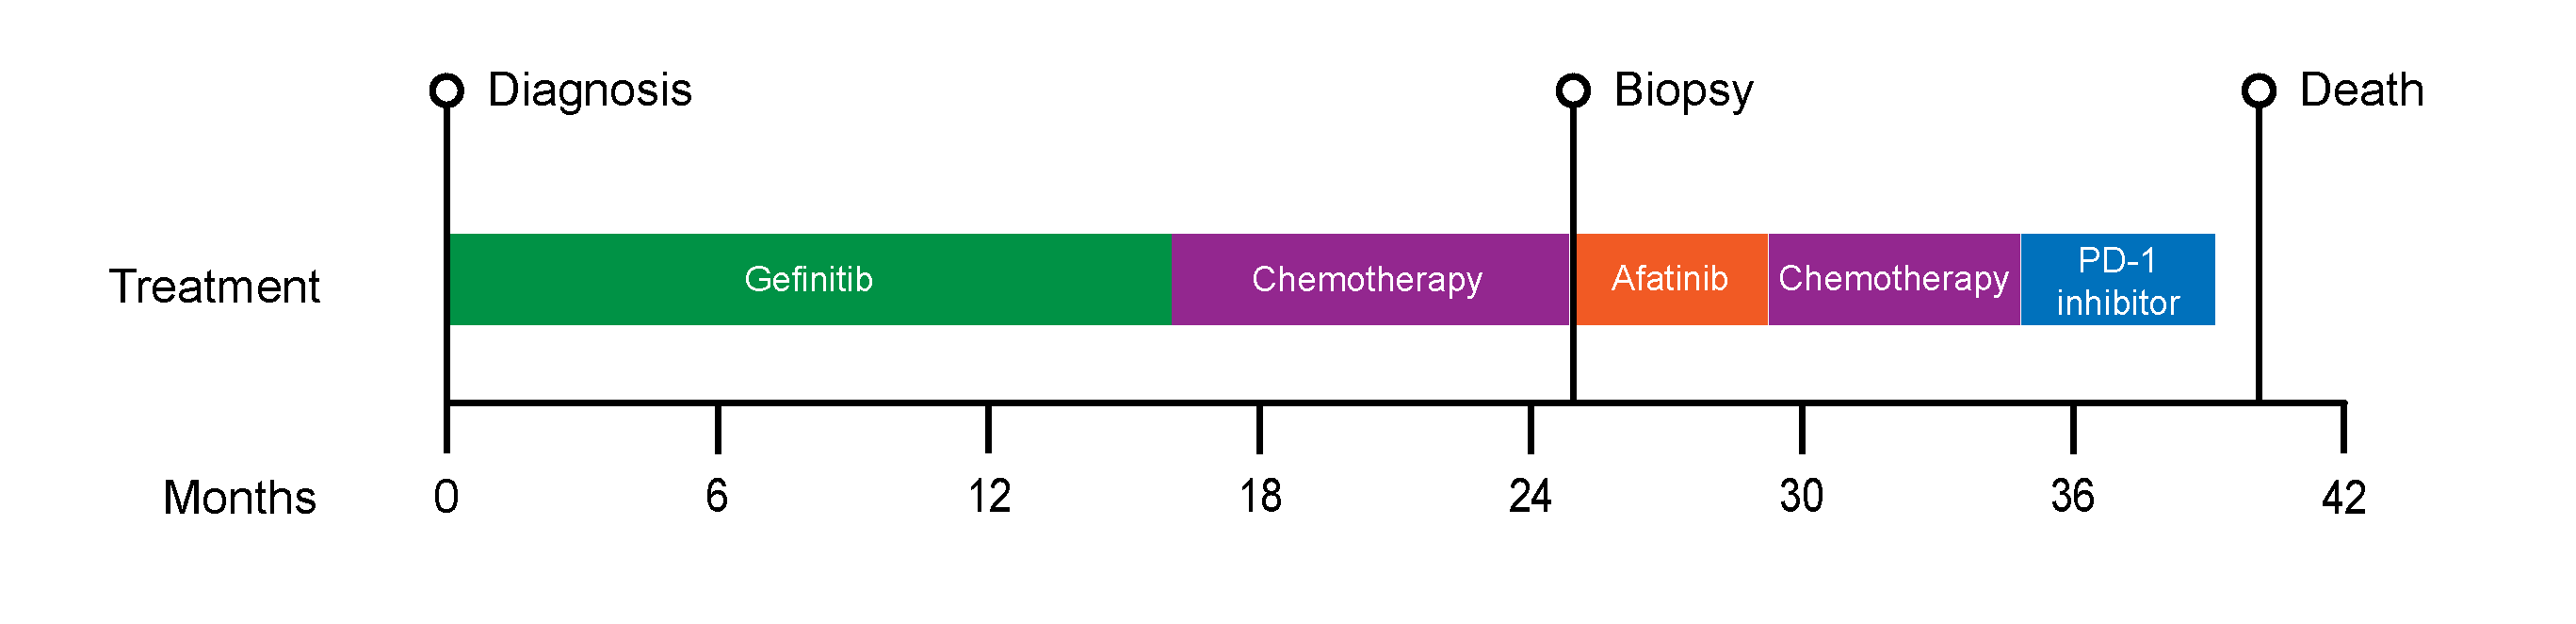
\includegraphics[width=.99\linewidth]{Figures/CA-I_timeline}
\caption[Timeline of patient CA-I from diagnosis until death]{Timeline of patient CA-I from diagnosis until death: Diagnostic biopsy detected EGFR exon 19 deletion lung adenocarcinoma; Second biopsy after 24 months revealed additional EGFR~T790M mutation and small cell transformation} \label{fig:ca51timeline}
\end{figure}



\begin{figure}[!ht]
\centering
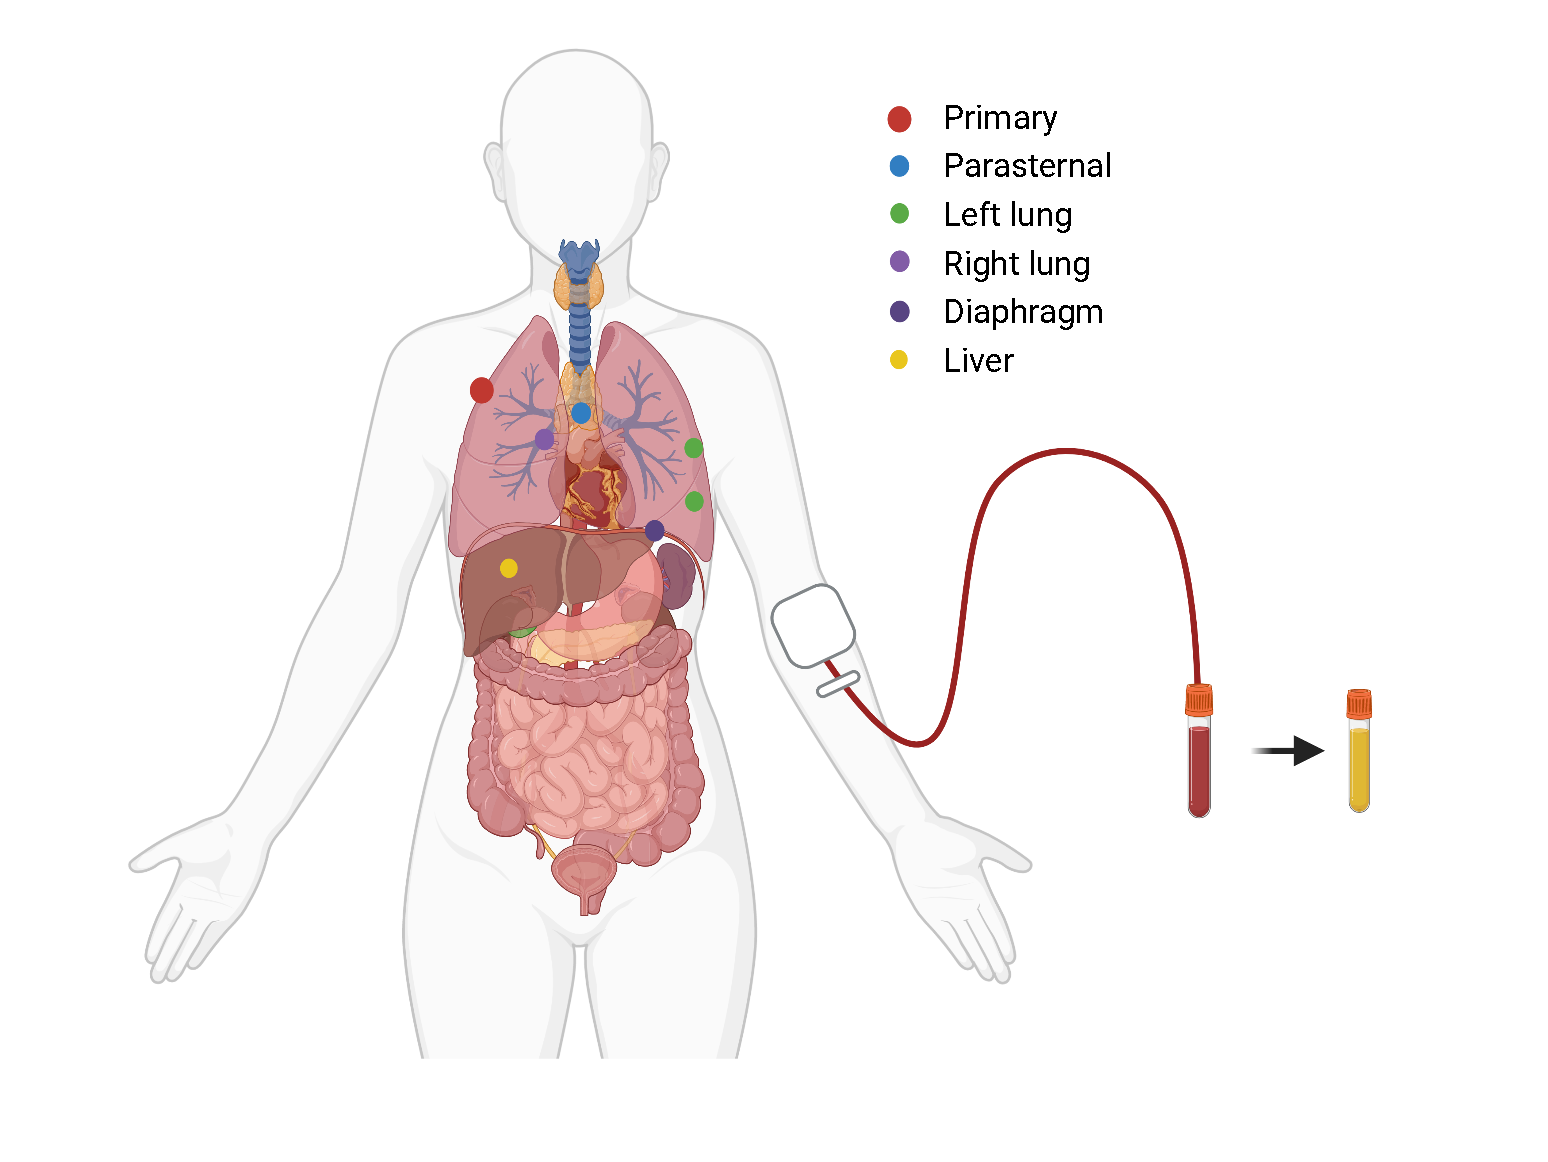
\includegraphics[width=.99\linewidth]{Figures/CA-I_schematic_CA51_organColours}
\caption[Schematic of tumour lesions in patient CA-I]{Schematic of tumour lesions in patient CA-I: Primary diagnostic sample shown in red; All six autopsy samples were coloured by organ they were collected from: Parasternal (1), left lung (2), right lung (1), diaphragm (1), liver (1); Additionally a post mortem blood sample was taken} \label{fig:cas51schematic}
\end{figure}


%we clear all floats before we go to the next patient
\cleardoublepage

\subsection{Patient CA-J}
\label{cascade-sec:CA80}


\begin{figure}[!ht]
\centering
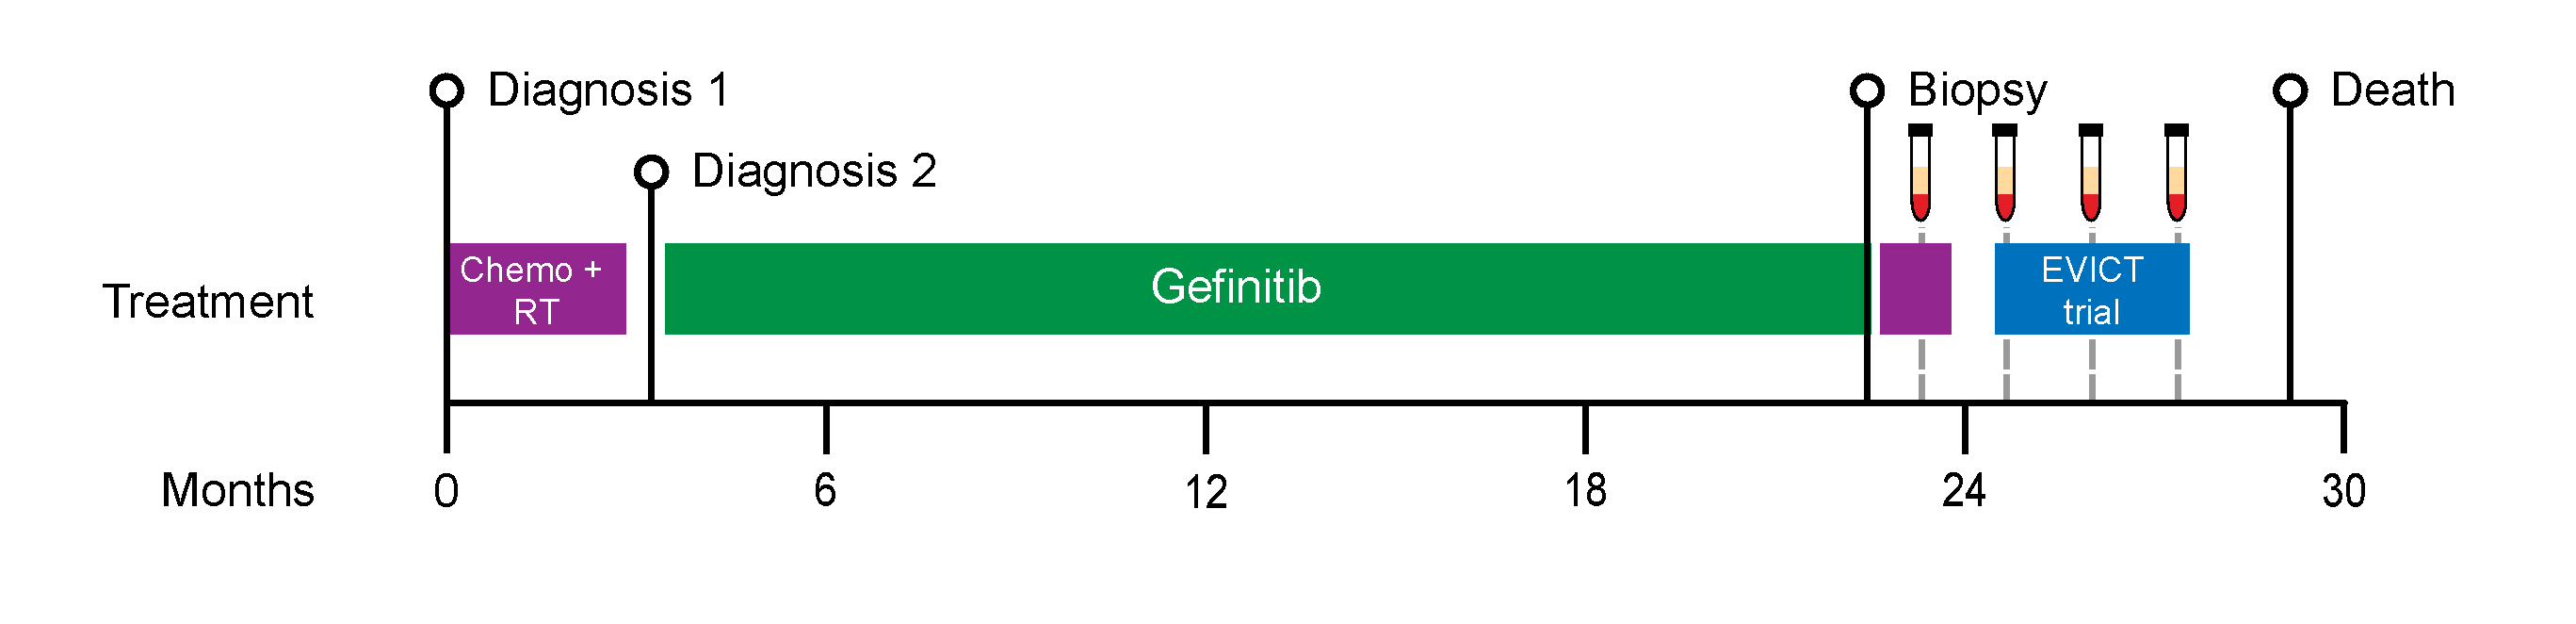
\includegraphics[width=.99\linewidth]{Figures/CA-J_timeline}
\caption[Timeline of patient CA-J from diagnosis until death]{Timeline of patient CA-J from diagnosis until death: Diagnostic biopsy detected EGFR~L858R positive stage IIIB lung adenocarcinoma; Second diagnosis after 3 months revealed additional brain and lung metastasis with a reclassification to stage IV; Biopsy at the end of erlotinib treatment revealed additional BRAF~V600E mutation; one blood sample was taken during the second round of chemotherapy and three more during the time the patient was enrolled in the EVICT trial} \label{fig:ca80timeline}
\end{figure}





\begin{figure}[!ht]
\centering
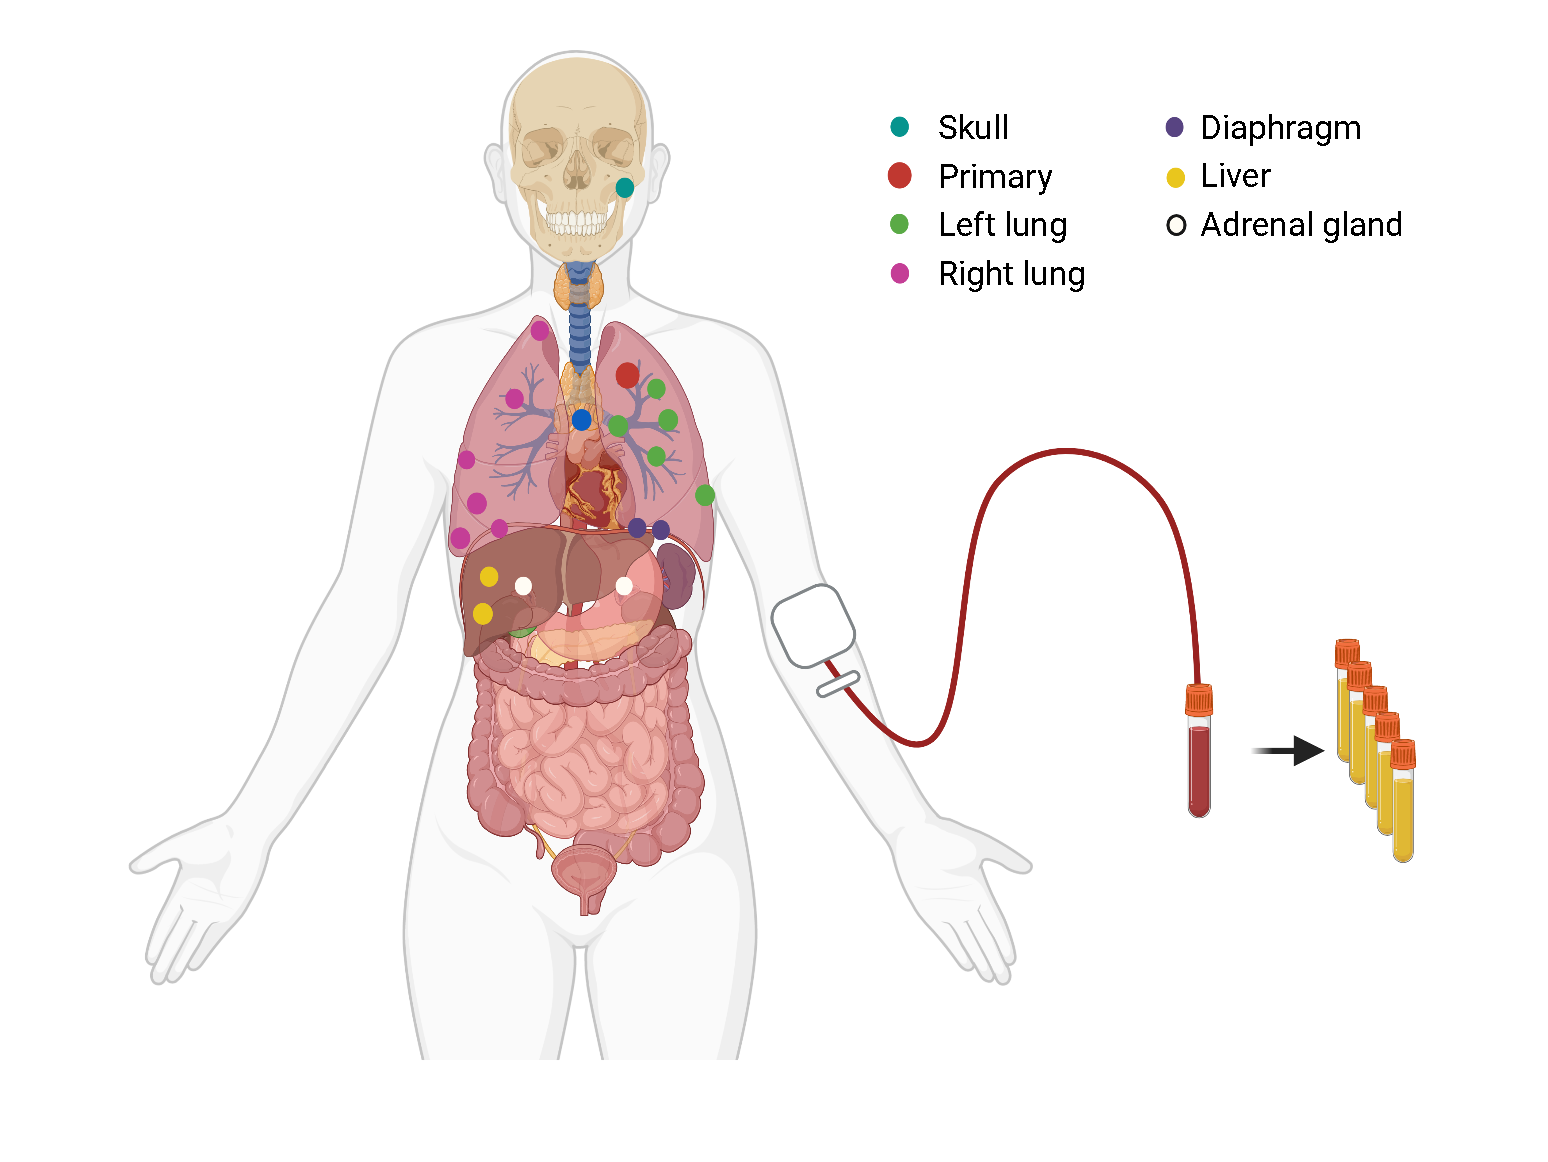
\includegraphics[width=.99\linewidth]{Figures/CA-J_schematic_CA80_organColours}
\caption[Schematic of analysed tumour lesions in patient CA-J]{Schematic of analysed tumour lesions in patient CA-J: Primary diagnostic sample shown in red; All 18 autopsy samples were coloured by organ they were collected from: skull (1), left lung(5), right lung (6), diaphragm (2), liver(2), adrenal gland (2); Additionally to the post mortem blood sample, four serial blood samples were taken (\protect\autoref{fig:ca80timeline})} \label{fig:cas80schematic}
\end{figure}


%we clear all floats before we go to the next patient
\cleardoublepage

\subsection{Patient CA-K}
\label{cascade-sec:CA82}

\begin{figure}[!ht]
\centering
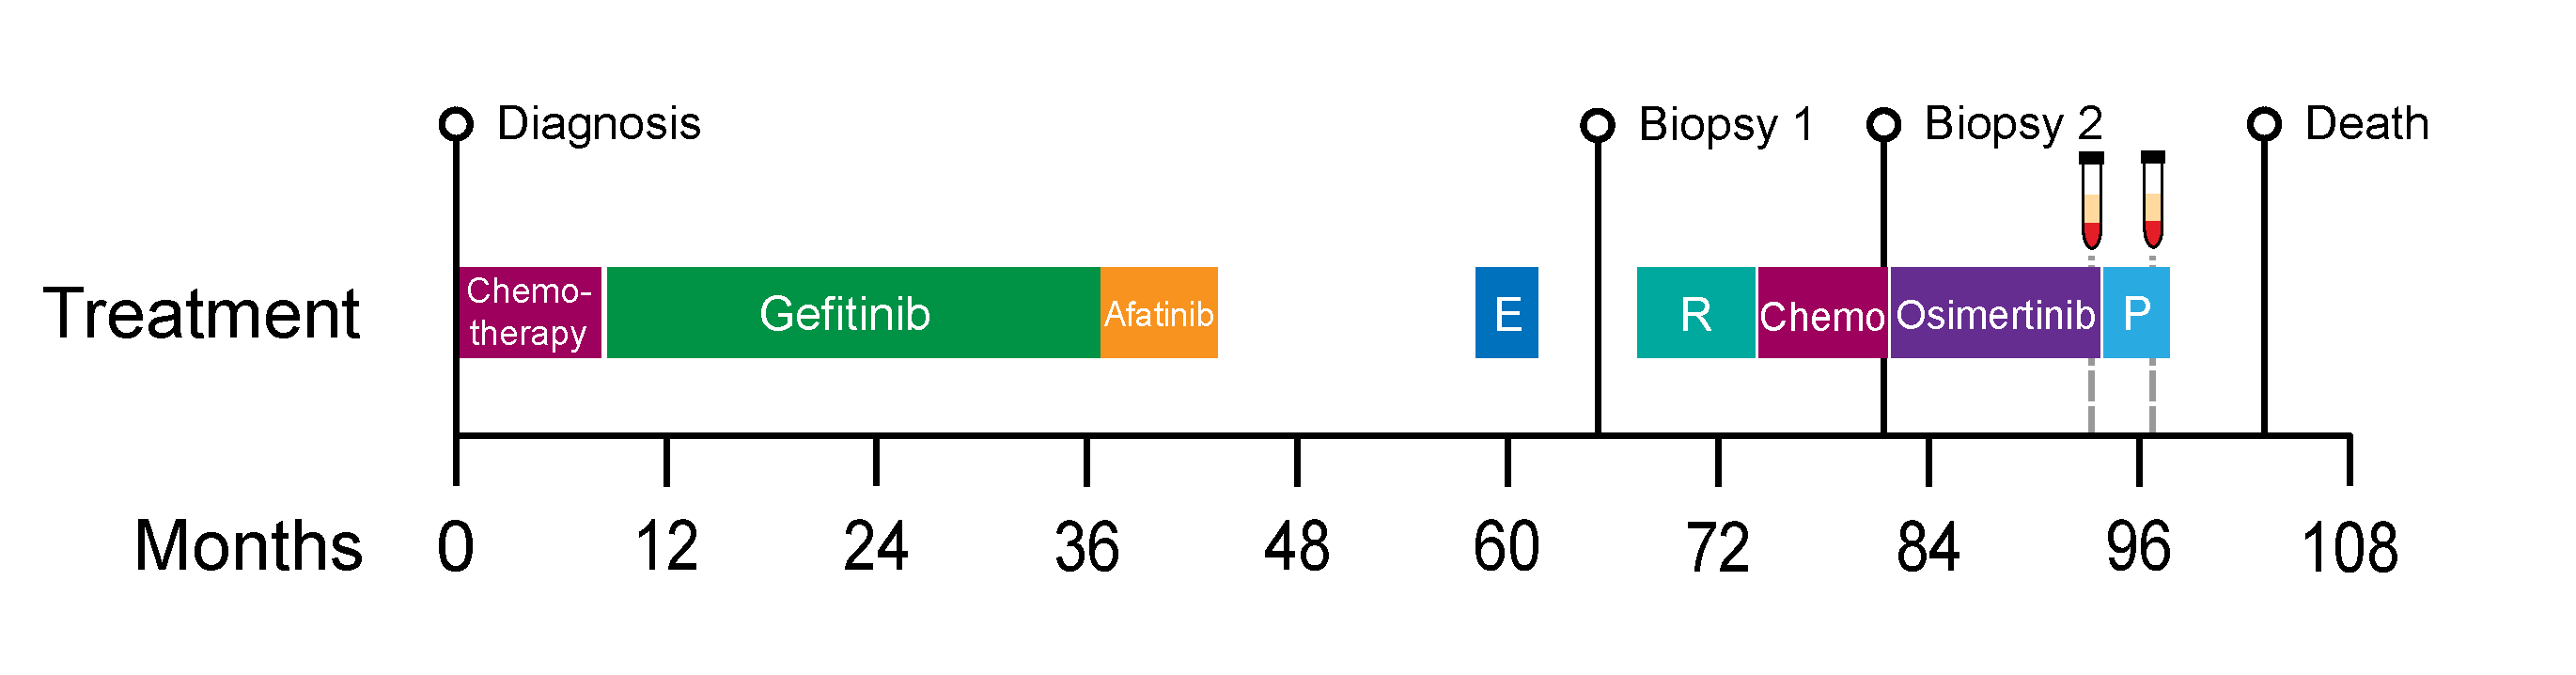
\includegraphics[width=.99\linewidth]{Figures/CA-K_timeline}
\caption[Timeline of patient CA-K from diagnosis until death]{Timeline of patient CA-K from diagnosis until death: Diagnostic biopsy detected EGFR~L858R positive lung adenocarcinoma;  Biopsy 1 after 66 months showed additional EGFR~T790M mutation; Biopsy 2 showed no additional variants; one blood sample was taken towards the end of Osimertinib treatment and one second one during PD-1 checkpoint blockade treatment. E: Erlotinib; R: Rociletinib; P: PD-1 inhibitor} \label{fig:ca82timeline}
\end{figure}




\begin{figure}[!ht]
\centering
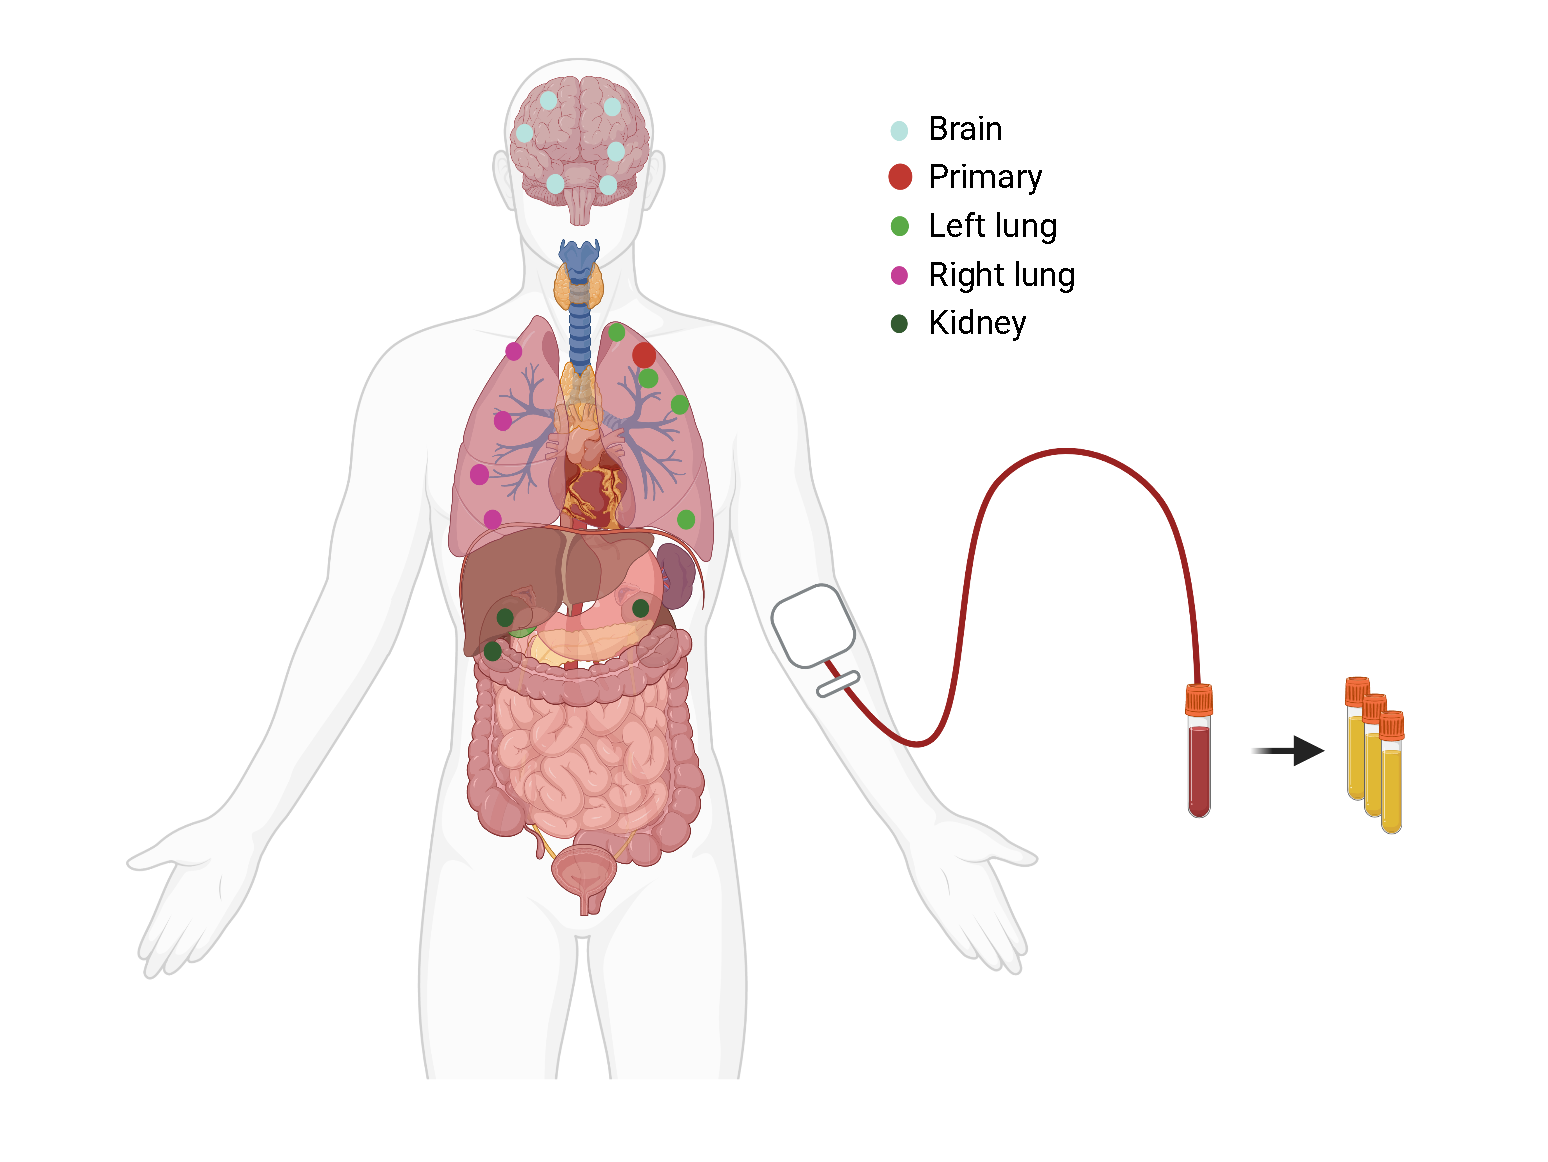
\includegraphics[width=.99\linewidth]{Figures/CA-K_schematic_CA82_organColours}
\caption[Schematic of analysed tumour lesions in patient CA-K]{Schematic of analysed tumour lesions in patient CA-K: Primary diagnostic sample shown in red; All 17 autopsy samples were coloured by organ they were collected from: Brain (6), left lung (4), right lung (4), kidney (3); Additionally to the post mortem blood sample, two serial blood samples were taken (\protect\autoref{fig:ca82timeline})} \label{fig:cas82schematic}
\end{figure}

%we clear all floats before we go to the next patient
\cleardoublepage

\subsection{Patient CA-L}
\label{cascade-sec:CA86}

This \todo{enter age} female patient presented with \textit{EGFR} mutant NSCLC, however after 12 months of the treatment with the EGFR inhibitor Erlotinib a transformation to small cell lung cancer (SCLC) was detected. While previously it was thought that the different subsets of lung cancers are distinct, more and more evidence is found showing neuroendocrine transformation as a resistance mechanism to targeted therapies not only in lung but also in prostate cancers \cite{Oser2015,Aggarwal2018}. The treatment was altered to chemotherapy and PD-1 inhibitors, however due to the loss of MHC-I antigen presentation of small cell lung cancer, the tumour failed to respond \cite{Burr2019} (\autoref{fig:ca82timeline}).

\begin{figure}[!ht]
\centering
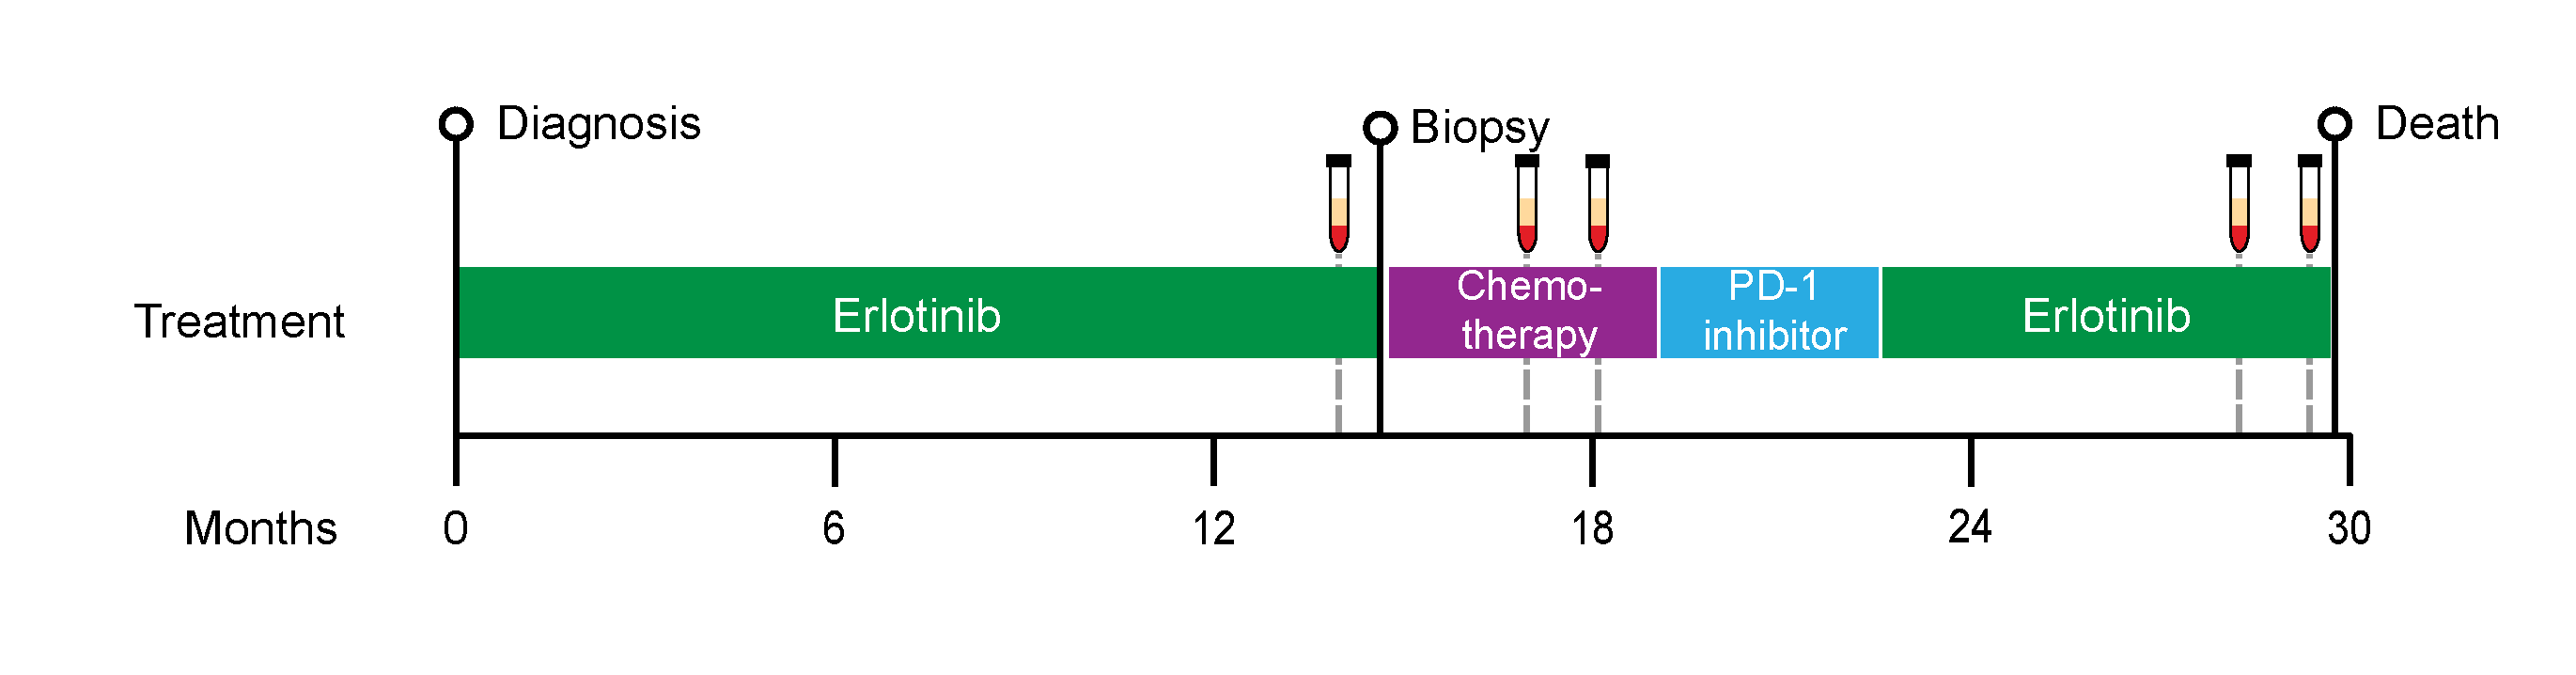
\includegraphics[width=.99\linewidth]{Figures/CA-L_timeline}
\caption[Timeline of patient CA-L from diagnosis until death]{Timeline of patient CA-L from diagnosis until death: Diagnostic biopsy detected EGFR exon 19 deletion positive lung adenocarcinoma;  Biopsy after 15 months Erlotinib treatment showed signs of small cell transformation; blood samples were taken at the end of the first Erlotinib treatment, during the chemotherapy treatment and  28 and 29 months after the initial diagnosis.} \label{fig:ca82timeline}
\end{figure}





\begin{figure}[!ht]
\centering
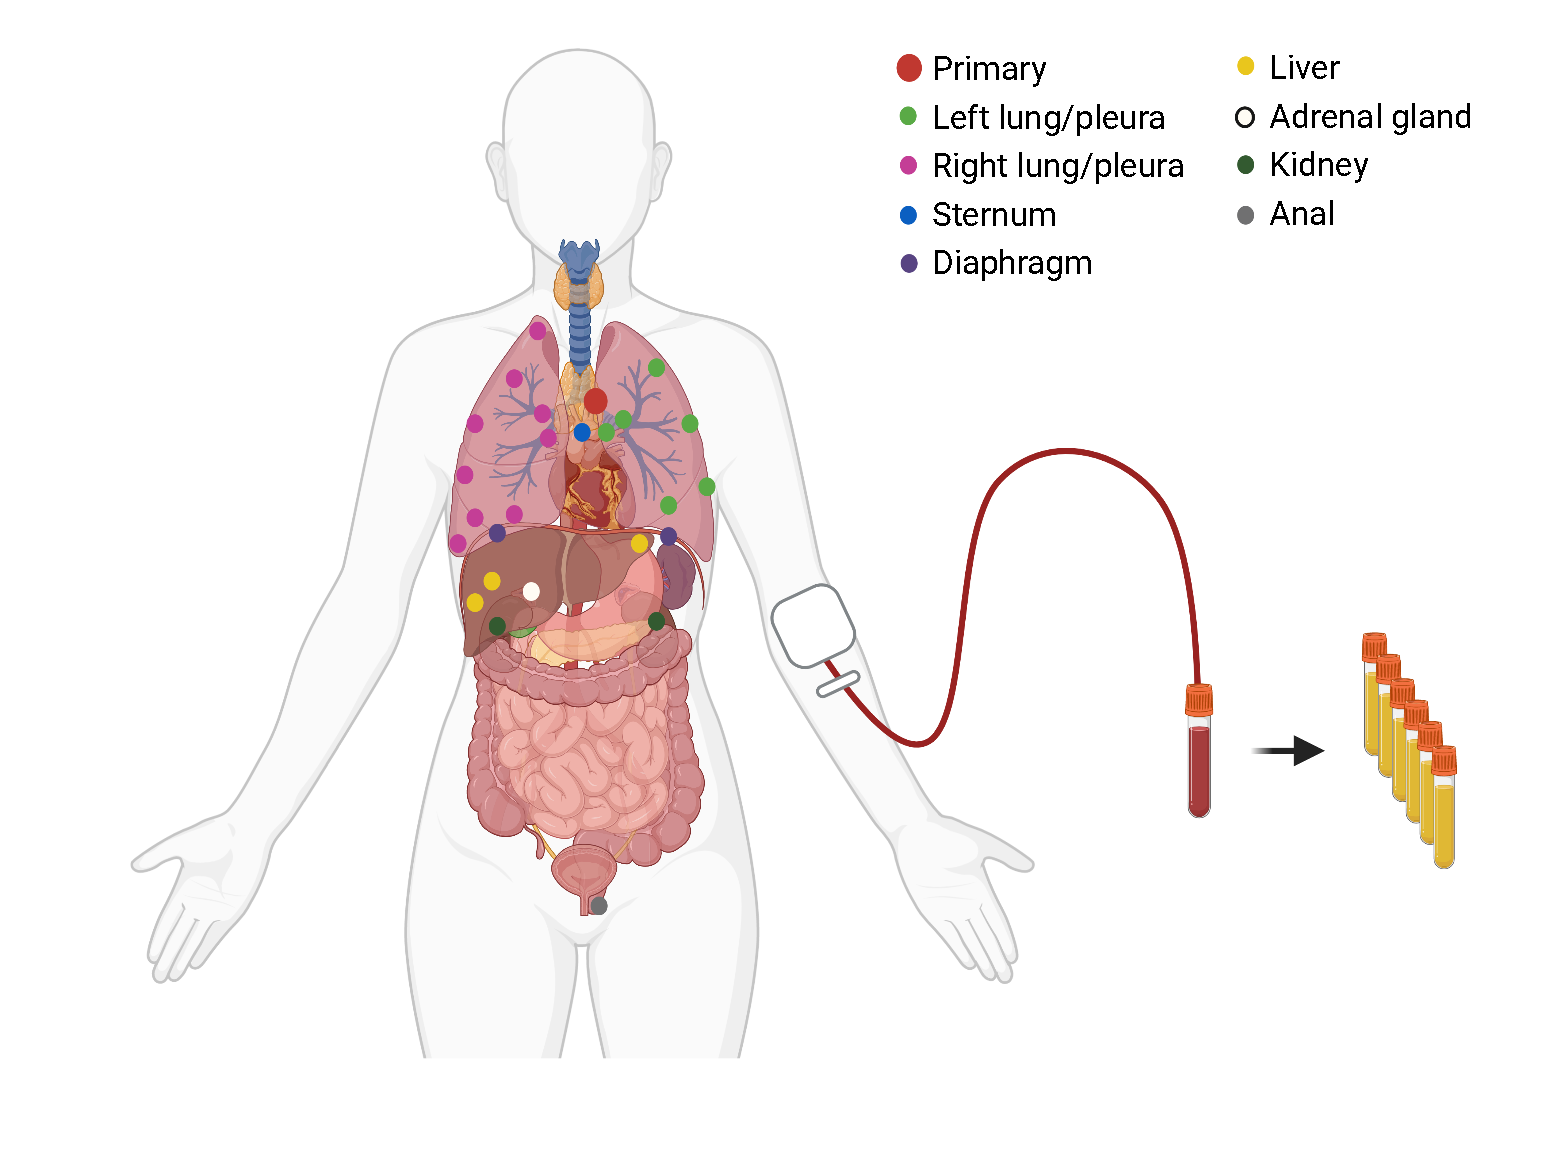
\includegraphics[width=.99\linewidth]{Figures/CA-L_schematic_CA86_organColours}
\caption[Schematic of analysed tumour lesions in patient CA-L]{Schematic of analysed tumour lesions in patient CA-L: Primary diagnostic sample shown in red; Samples are coloured by organ they were collected from: left lung (6), right lung (9), sternum (1), diaphragm (2), liver (3), adrenal gland (1) kidney (2), anal (1); Additionally to the post mortem blood sample, five serial blood samples were taken (\protect\autoref{fig:ca86timeline})} \label{fig:cas86schematic}
\end{figure}



%we clear all floats before we go to the next section
\cleardoublepage

\section{Cohort level analysis}
\label{cascade-sec:cohortLevel}

\todo[inline]{short explanation about what this does}


\subsection{Phylogenetic reconstruction}
\label{cascade-sec:phylo}

\todo[inline]{Phylogenies and comparisons}

% the analysis about mitochondrial phyolgenies
\section[Mitochondrial phylogenetic reconstruction]{Mitochondrial phylogenetic reconstruction - the power house of the phylogenies}
\label{cascade-sec:mitochondria}

While phylogenetic reconstruction is a well-established method for genetic variants from canonical chromosomes to study metastatic progression and timing of evolutionary divergence \cite{Deshwar2015,Brown2017,Hu2019}, there are multiple issues. In \autoref{variantcalling-sec:phylo} and \autoref{variantcalling-sec:clonal}, we showed how important the proper variant calling method is to \remove{accurately} recover phylogenies and clonal patterns\add{ accurately}. In addition, using somatic variants to reconstruct phylogenies is a flawed concept to begin with. 

Most models studying genetic variation assume neutral evolution of the DNA loci \cite{Kimura1968,Lynch1989}, but cancers almost exclusively exhibit positive selection \cite{Cannataro2018}. \change{And}{Moreover,} while passenger mutations might not directly affect \add{the} \change{fitness of the cell}{cell's fitness}, they only exist due to the link to the driver mutation and \remove{therefore} provide little to no additional information gain in addition to the driver. Furthermore, while in small populations, genetic drift as a stochastic process overpowers selective processes (fitness coefficient $s$) and can therefore be assumed to be neutral, in larger populations $N_e$ (effective population size) where \autoref{mmf-eq:neutralSelection} does not hold true, mutations are under selective pressure \cite{EyreWalker2007}.
\begin{equation}
N_e \cdot s \ll 1 \label{mmf-eq:neutralSelection}
\end{equation}
\myequation[\ref{mmf-eq:neutralSelection}]{Selective pressure with effective population size}
%we need to squish this a bit otherwise it looks weird
\vspace{-3em}
In summary, we can assume that with cancer cell growth, positive selection through treatment, and tumour-microenvironmental niches, almost all assumptions of the coalescent theory \cite{Kingman1982} are not applicable for tumour samples and therefore, methods using somatic variants and their respective results need to be selected and evaluated carefully.

To tackle this issue and assist with \change{the interpretation of}{interpreting} phylogenetic reconstruction results, we adjusted a method used in single-cell sequencing to track clonal expansion with mitochondrial somatic mutations \cite{Ludwig2019} to be usable \change{for}{with} standard bulk sequencing. Mitochondrial variants are an ideal source of clonality information because the mutation rate is significantly higher than nuclear DNA due to the missing proofreading and repair mechanisms, \change{which allows}{allowing} very granular separation in a shorter time\remove{ period}. Additionally, while \remove{there are several diseases caused by} defects in mitochondria\add{ cause several diseases}, such as Kearns-Sayre syndrome \cite{Harvey1992}, MERRF \cite{Adam1993} and MELAS \cite{Hirano1992}, they usually follow a mendelian inheritance pattern and are hereditary and not somatically acquired. In the cancer context, somatic mutations in mitochondrial DNA are assumed to be approximately neutral, with a possible selection pressure towards healthy ageing and negative selection in cancer \cite{Rodell2013,Yuan2020}.

\subsection{Method}
\label{cascade-sec:mitoMethod}

First, a pileup of all mitochondrial positions was performed. Before, the pileup we preselected reads which uniquely mapped to the mitochondrial genome and only retained high mapping-quality reads. Then the nucleotide counts in each position were transformed into a MultiEssayExperiment \cite{Ramos2017} for final analysis in R. The preprocessing code can be found in \autoref{lst-cascadeAppendix:mitoPreProcessing}.

The final MultiEssayExperiment was then read into R, and quality metrics \add{were }applied to exclude samples with \change{not enough}{insufficient} coverage on the mitochondrial contig. Our analysed WGS samples showed an extensive coverage of mitochondrial DNA\change{, however}{. However}, WES library preparation procedures might restrict coverage through hybridisation pulldown. Patient CA-I had \remove{a coverage of} more than 100x \add{coverage }for all but the germline sample, which only had an overall coverage of 17x. Similarly, patient CA-L showed lower depth for the germline sample (127x) but a generally high coverage for all tumour samples (mean: 543x, min: 138x). All other Patients (CA-A/J/K) where samples were sequenced with WGS exhibited a coverage of more than 200x, even for low-performing samples with a median depth of \num{67916}, \num{45603}, and \num{49726} per sample~(\autoref{fig:mtCoverage}).

\begin{figure}[hbt]
\centering
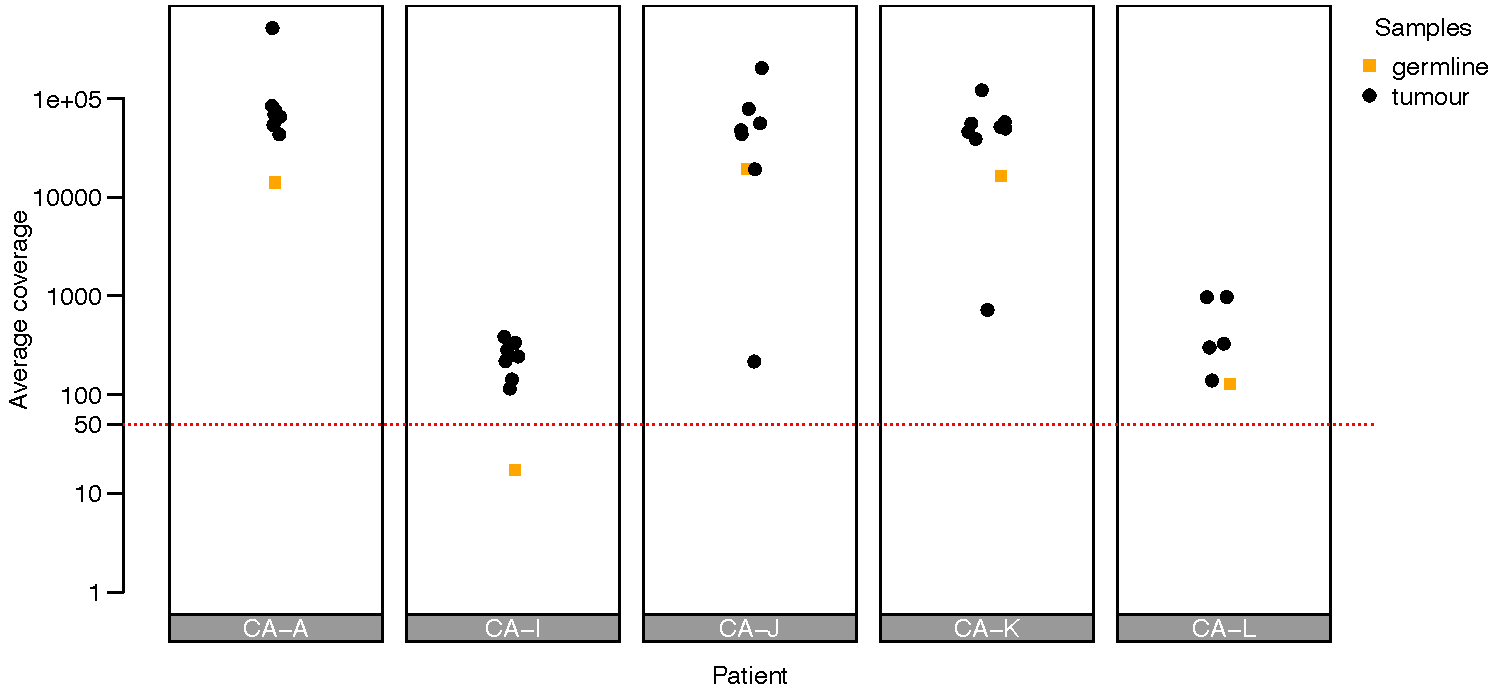
\includegraphics[width=.99\linewidth]{Figures/CASCADE/mito/mtCoverage}
\vspace{-1em}
\caption[Average coverage of mitochondrial DNA of CASCADE patients]{Average coverage of mitochondrial DNA of CASCADE patients: Orange squares show germline sample for each patient; black points show tumour samples; horizontal red dotted line shows quality cut off suggested by \protect\textcite{Ludwig2019}} \label{fig:mtCoverage}
\end{figure}


Th\change{is}{ese metrics} proved that even without specifically enriching for mitochondrial DNA, most samples \remove{will }contained enough tumour reads for this analysis.

To ensure optimal results, we excluded all samples with an average coverage of less than 50x. This exclusion meant we removed the germline sample for patient CA-I\change{, h}{. H}owever, as we expected the germline sample to be the ancestral state for all samples, this has virtually no effect on the reconstruction procedure. Additionally, we were more interested in the relationships between the tumour sample, which was still accessible even with the removed germline sample.

In contrast to the simple Hamming distance used for the presence-absence vector representation of canonical somatic variants (\autoref{cascade-sec:phylo}), for mitochondrial variants, we employed an allele frequency ($vaf$) based distance (\autoref{eq:mitoDist}) of two samples~$s_i$ and $s_j$. The difference in read support was normalised with the product of the total allelic depth~$cov$ and summed up at all sites of variation~$v$.

\begin{equation}
mitoDist(s_i,s_j) = \sum_{v \in Variants} \left| \frac{vaf_{s_i}(v) \cdot cov_{s_i}(v) - vaf_{s_j}(v) \cdot cov_{s_j}(v)}{cov_{s_i}(v) \cdot cov_{s_j}(v)} \right| \label{eq:mitoDist}
\end{equation}
\myequation[\ref{eq:mitoDist}]{Mitochondrial variants based distance function of two samples}

This distance was only calculated for variant sites where both samples had at least a coverage of 100x to have a representative sampling of the allelic prevalence in each sample, as a human cell usually has more than 100 mitochondria \cite{Cole2016}.


\subsection{Results}
\label{cascade-sec:mitoResults}
While the mitochondrial variants analysis only used a fraction of the size of the genomic DNA loci and therefore most likely violates the infinite sites assumption \cite{Kimura1969}, it was still able to generate an orthogonal view of the heterogeneity and trajectory of the multi-regional samples in each patient.

\subsubsection{Patient CA-A}

While the separation of progression (11, 47, 55, and 59) and stable (26, 31, 41, and 57) disease sites was already visible in the somatic phylogeny, the bottleneck of treatment and new metastasis is more \change{obvious}{evident} in the mitochondrial phylogeny. However, the individual resolution of splits appeared to be lower for the mitochondrial reconstruction, as seen in \autoref{fig:CA99mitoPhylo}.


\begin{figure}[h]
\centering
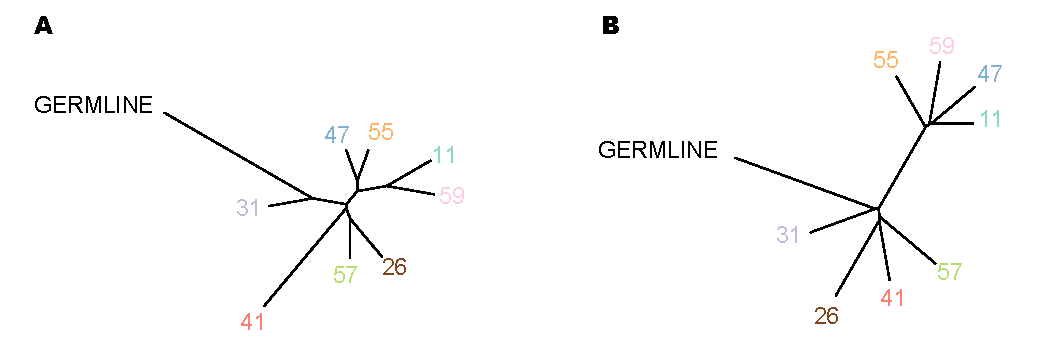
\includegraphics[width=.99\linewidth]{Figures/CASCADE/mito/CA99SomVsMitoPhylo.pdf}
\caption[Mitochondrial and somatic phylogenetic reconstruction of CA-A]{Mitochondrial and somatic phylogenetic reconstruction of CA-A: Somatic variants based reconstruction (A) and mitochondrial variants based reconstruction (B)} \label{fig:CA99mitoPhylo}
\end{figure}

\subsubsection{Patient CA-I}

Neither the somatic \remove{variants} nor the mitochondrial variants resolved the evolutionary trajectory in a granular fashion. The slightly longer stem of shared variants in the mitochondrial phylogeny was most likely due to the low coverage of the germline sample. Similar to all other patients, the substructure of the samples was changed. While \remove{using} the somatic variants showed sample 566 as the closest to the germline sample, the mitochondrial variant phylogeny instead indicated sample 559 as the closest (\Autoref{fig:mtCoverage,fig:CA51mitoPhylo}).


\begin{figure}[ht]
\centering
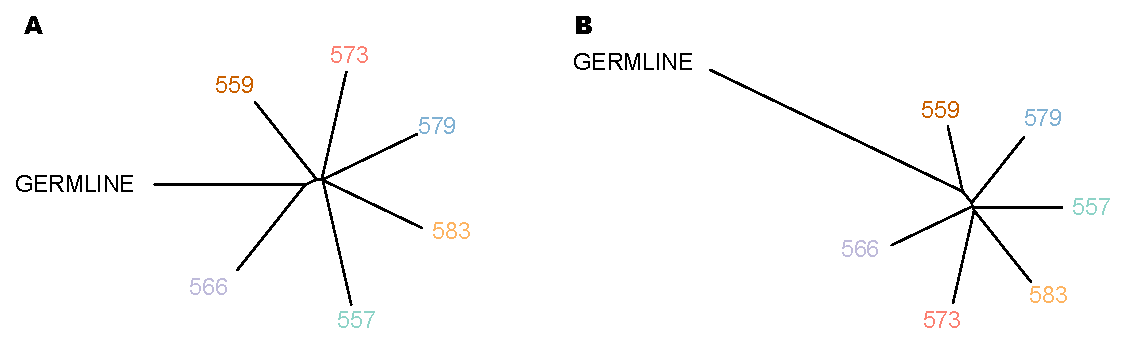
\includegraphics[width=.99\linewidth]{Figures/CASCADE/mito/CA51SomVsMitoPhylo.pdf}
\caption[Mitochondrial and somatic phylogenetic reconstruction of CA-I]{Mitochondrial and somatic phylogenetic reconstruction of CA-I: Somatic variants based reconstruction (A) and mitochondrial variants based reconstruction (B)} \label{fig:CA51mitoPhylo}
\end{figure}


\subsubsection{Patient CA-J}

The mitochondrial reconstruction presented sample 2 as a member of the more genetically complex samples 20, 24, 32, and 42 \change{in spite of}{despite} the missing \textit{TP53} mutation. Sample 28, on the other hand, \remove{which }showed almost no evolutionary distance to the normal sample in the somatic analysis, \add{but} presented as a substantial outlier\add{ in the mitochondrial data}. This disconnect showed that the TP53 mutations of samples 20, 24, 32, and 42 \change{was}{were} likely acquired after the seeding of the distant sites like sample 2 in the adrenal gland. The difference in distance to the normal sample for sample 28 was likely due to a ``cold`` primary site of disease with little cell proliferation, which\remove{, however,} still accumulated mitochondrial mutations \cite{Abascal2021} (\autoref{tab:ca80cnv}, \autoref{fig:CA80mitoPhylo}).

\begin{figure}[ht]
\centering
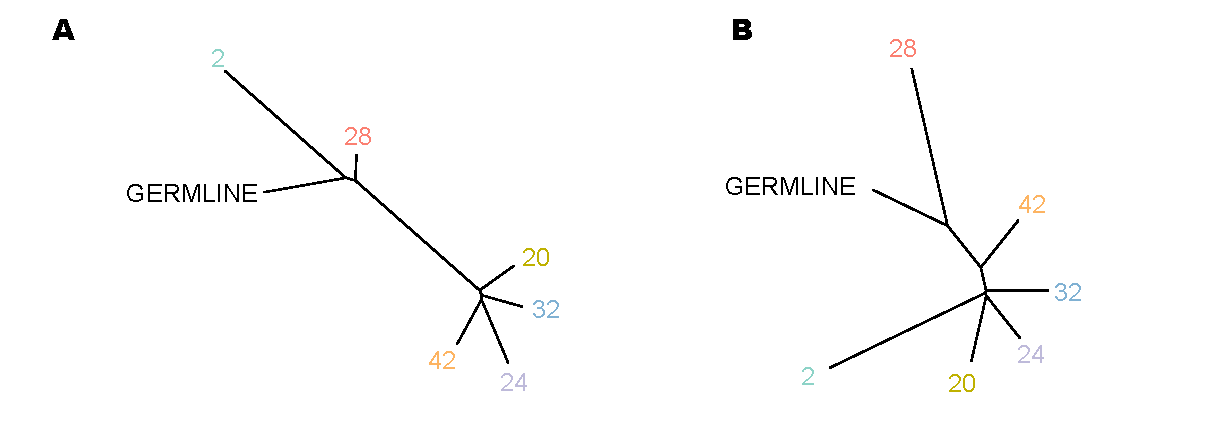
\includegraphics[width=.99\linewidth]{Figures/CASCADE/mito/CA80SomVsMitoPhylo.pdf}
\caption[Mitochondrial and somatic phylogenetic reconstruction of CA-J]{Mitochondrial and somatic phylogenetic reconstruction of CA-J: Somatic variants based reconstruction (A) and mitochondrial variants based reconstruction (B)} \label{fig:CA80mitoPhylo}
\end{figure}


\subsubsection{Patient CA-K}

In contrast to the somatic variant phylogeny, which showed an outgroup of samples 8 and 9, with a second cluster of samples 4, 5, and 6, the mitochondrial data supported a different  split into two groups. These groups almost perfectly bifurcated the samples into those derived from the left and right sided disease sites, with sample 6 being the only sample from  the right side clustered with the left lung and brain samples 8, 9, and 13. These data suggested that while only samples 8 and 9 showed a whole genome duplication and the \textit{APC} ``stop gained`` mutation, they were more closely related to the other samples than assumed from the somatic variant analysis and probably were seeded by the same cells (\autoref{tab:ca82cnv}, \Autoref{fig:ca82heatmap,fig:CA82mitoPhylo}).

\begin{figure}[ht]
\centering
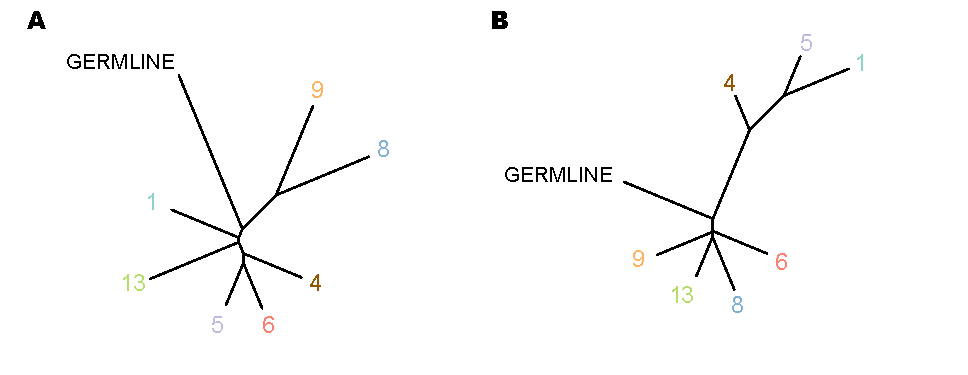
\includegraphics[width=.99\linewidth]{Figures/CASCADE/mito/CA82SomVsMitoPhylo.pdf}
\caption[Mitochondrial and somatic phylogenetic reconstruction of CA-K]{Mitochondrial and somatic phylogenetic reconstruction of CA-K: Somatic variants based reconstruction (A) and mitochondrial variants based reconstruction (B)} \label{fig:CA82mitoPhylo}
\end{figure}


\subsubsection{Patient CA-L}
While the somatic variants linked the small cell carcinoma samples P.1 and 8 together, the mitochondrial analysis showed that the closest relative to P.1 was P.2. As both of the progression samples were taken 14 months ahead of the death of the patient, this agreed with the clinical history of the samples better. Additionally, instead of grouping the\remove{ the} adenocarcinoma samples 17A and 26\remove{ together}, the mitochondrial phylogeny suggested that while they share a common resistance mechanism (EGFR~T790M), it might have been acquired in parallel instead of being seeded from the same lesion, as all samples other than the P.1/2 samples were not grouped\remove{ together}. Lastly, the closeness of sample 8 and the germline sample possibly indicated the presence of small cell disease already ``before`` the progression samples were collected. However, the FFPE conservation of the P samples could have altered the molecular clock and influenced the branching site on the tree (\Autoref{fig:ca86heatmap,fig:CA86mitoPhylo}).

\begin{figure}[ht]
\centering
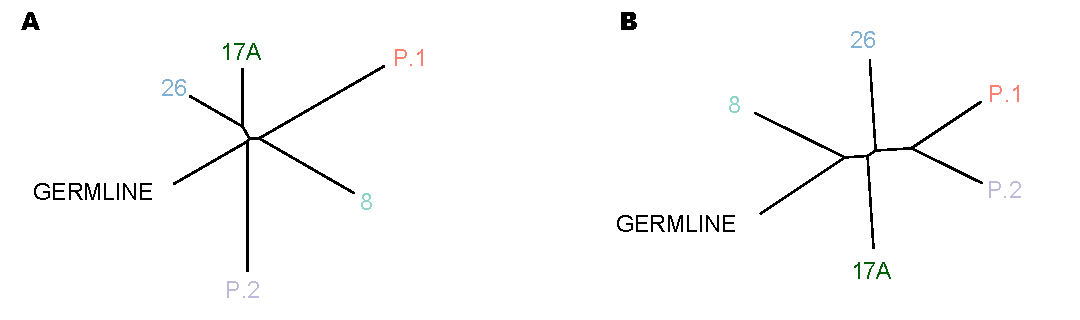
\includegraphics[width=.99\linewidth]{Figures/CASCADE/mito/CA86SomVsMitoPhylo.pdf}
\caption[Mitochondrial and somatic phylogenetic reconstruction of CA-L]{Mitochondrial and somatic phylogenetic reconstruction of CA-L: Somatic variants based reconstruction (A) and mitochondrial variants based reconstruction (B)} \label{fig:CA86mitoPhylo}
\end{figure}

\subsection{Summary}
With the analysis of the mitochondrial history of samples, we could shed some light on the timing of lesions and the development of resistance mechanisms, which is not heavily influenced by the treatment and its selection pressure. While the infinite sites hypothesis does not hold true for mitochondrial DNA, due to the limited sites and reduced repair mechanisms, the selection pressure of treatment and their resistance mechanisms parallel evolution bias in the analysis of multiple related tumour samples also violates multiple assumptions for phylogenetic reconstruction when using somatic variants. 

\note{massive rewrite}Neither options come without pitfalls and caveats, but this method could offer an alternate view on the history and seeding time of lesions and their kinship using data that was previously discarded but was abundantly available. This approach is also available at virtually no additional cost, as mitochondrial variants can be readily detected from standard WGS and WES. As mitochondrial DNA analysis has recently been moved into the spotlight as a biomarker for stress and mortality \cite{Trumpff2021} and other diseases \cite{Cushen2022}, we were interested similar to see if tissue mitochondrial DNA analysis, like circulating mitochondrial DNA, could unlock another multi-omics dimension. Furthermore, mitochondrial DNA was successfully used to distinguish clones in single-cell sequencing \cite{Ludwig2019}. 

While certain aspects of evolutionary trajectory and patterns are conserved between the nuclear DNA and the mitochondrial DNA, many are not. These differences might be caused by the reduced granularity of the mitochondrial analysis, where the median number of somatic variants was 345 (min: 128, max 5401) over the median of 23252 (min: 10947, max: 64580) in the nuclear DNA, however they could also be caused by a different biological process. The method is not an alternative to nuclear DNA phylogeny, but rather points out a need for further investigation. The reconstruction methods should be approximately equivalent with the current biological insight. However, the discrepancy of results from nuclear and mitochondrial DNA phylogenetic reconstruction, warrants further investigation of mitochondrial evolution in the cancer setting, outside the scope of this work.

% the missing analysis?
\section{Outlook}
\label{cascade-sec:outlook} 


\begin{savequote}[65mm]
``Many a mickle makes a muckle.``
\qauthor{--- proverb}
\end{savequote}


\chapter[Mismatchfinder]{MisMatchFinder - hope springs eternal}
\label{ch:mmf}

%\epigraph{``Many a mickle makes a muckle.``}{--- \textup{proverb}}

% introduction into the idea of the chapter
\section{Introduction}
\label{mmf-sec:intro}

Early researchers and physicians realised that cancers can have different morphologies and clinical progression depending on the primary occurrence of the tumour (\autoref{intro-sec:cancer})\change{, w}{. W}ith the extensive sequencing of cancer specimens over the last two decades, the mutational signatures of cancers came into focus. These signatures are specific and characteristic combinations of mutations, which stem from distinct biological processes. These processes include exposure to DNA-damaging agents like chemotherapy treatment, tobacco and UV radiation, and biological intrinsic pathway errors in DNA replication or repair. As each of those processes has a more or less distinct profile of mutations \cite{Hollstein1991,Kucab2019}, the analysis and deconvolution of the signatures contributing to a patient's mutational landscape can help to diagnose and treat a patient. While many signatures occur at a background level and are related to ``normal`` cellular processes like ageing \cite{Alexandrov2013}, others can point to defective mismatch repair or gain of function mutations in specific pathways, which can lead to new avenues of therapy for a patient \cite{Neil2017}.

Supplementary information and plots for this chapter are attached in the appendix and prepended with \ref{ch-mmfSuppMeth}.

\subsection{Mutational signature analysis}
\label{mmf-sec:signatureanalysis}
Traditionally cancer mutational signature analysis entails a somatic variant calling process (\autoref{intro-sec:variantcalling}) followed by a counting and deconstruction step, which assigns weights to the individual signatures. These signatures are a pre-compiled list of mutation count relations (\autoref{fig:sig7a}). While individual SNPs already contain valuable information, there is an improvement in signature granularity when \remove{also }counting the base up and downstream of the nucleotide change. Th\change{is}{ese additonal bases} expand\remove{s} the feature space of counts from the six base classes of SNPs (C>A, C>T, C>G, T>C, T>A, and T>G) to 96 unique trinucleotide contexts \cite{Alexandrov2013}. While there technically are six more base changes and several  more trinucleotide contexts combinatorially possible, they can be collapsed into the \remove{aforementioned} 96 \add{mentioned above} by using the reverse complement of the change.

\begin{figure}[!ht]
\centering
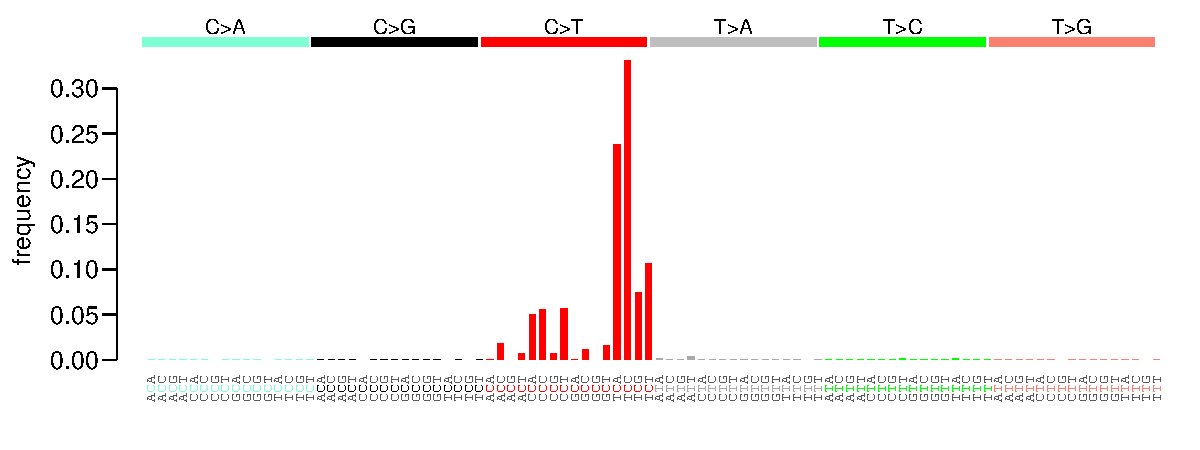
\includegraphics[width=.99\linewidth]{Figures/MisMatchFinder/SBS7aSignature.pdf}
\caption[Trinculeotide count contributions for single base substitution (SBS) signature 7a]{Trinculeotide count contributions for SBS signature 7a (UV exposure); values taken from \protect\textcite{Alexandrov2020}}\label{fig:sig7a}
\end{figure}

Additionally to the single base substitution (SBS), there exists doublet base substitution signatures (DBS) and InDel signatures for somatic mutations of cancers \cite{Alexandrov2020}, which are all based on the same principle and enable a higher precision for stratification of similar cancer subtypes and DNA damaging agents.

\subsection{Restrictions and pitfalls of standard signature analysis}
Especially for cancer samples, the focus, when analysing mutational signatures, is on somatic variants of the sample. \change{This}{Somatic variant calling, however,} requires deep sequencing of the tumour sample with at least WES or WGS. For optimal results, a  matched germline sample for tumour-normal variant calling is required (\autoref{intro-sec:somaticcalling}). This means the \change{cost of the assay}{assay cost} is surprisingly high for the diffuse result of signature contributions of the variants in the sample. This \add{cost overhead }is especially relevant when it comes to clinical diagnostic tools, where every biopsy of the patient is precious and not easily obtained. Additionally, the matched germline sample might not be available. For an analysis\remove{, which is} based on the averaged and aggregated somatic variants\change{, to require a}{ requiring} high-quality input \change{could be seen as}{is} counter-intuitive. \change{Especially}{Particularly} as the current gold standard analysis will report signatures, even if \change{there are virtually no variants}{virtually no variants are} reported\change{. W}{, w}e \remove{therefore} developed a method \change{which}{that} can be adapted for low coverage whole genome sequencing and requires no prior knowledge of the cancer or \change{a}{the} germline sample. \add{With this new method, we were able to analyse sequencing data, where normal variant calling is not possible due to the low and sparse read coverage.}

\subsection{Overview}
This chapter describes a newly developed method\change{, which}{ that} allowed the detection of somatic signatures from low-coverage WGS of cfDNA. \change{This method, w}{W}ith further optimisation and validation, \change{has the potential to}{this method can} provide a novel approach for non-invasive monitoring of patients and  screening of at-risk individuals in a clinical setting.


% more things, when the story is clear if i just write what i have done and no publication 

\chapter{Conclusion}
\label{ch:conclusion} % 

%% ----------------------------------------------------------------
% Now begin the Appendices, including them as separate files

\addtocontents{toc}{\vspace{2em}} % Add a gap in the Contents, for aesthetics

\appendix % Cue to tell LaTeX that the following 'chapters' are Appendices

%\input{Appendices/AppendixA}	% Appendix Title

%\input{Appendices/AppendixB} % Appendix Title

%\input{Appendices/AppendixC} % Appendix Title

\addtocontents{toc}{\vspace{2em}}  % Add a gap in the Contents, for aesthetics
\backmatter

%% ----------------------------------------------------------------
\label{Bibliography}
\lhead{\emph{Bibliography}}  % Change the left side page header to "Bibliography"
\printbibliography

\end{document}  % The End
%% ----------------------------------------------------------------
